\documentclass[lang=cn,10pt]{elegantbook}
\usepackage{subfigure}
% 定义可能使用到的颜色
\definecolor{CPPLight}  {HTML} {686868}
\definecolor{CPPSteel}  {HTML} {888888}
\definecolor{CPPDark}   {HTML} {262626}
\definecolor{CPPBlue}   {HTML} {4172A3}
\definecolor{CPPGreen}  {HTML} {487818}
\definecolor{CPPBrown}  {HTML} {A07040}
\definecolor{CPPRed}    {HTML} {AD4D3A}
\definecolor{CPPViolet} {HTML} {7040A0}
\definecolor{CPPGray}  {HTML} {B8B8B8}
\lstset{
    columns=fixed,       
    numbers=left,                                        % 在左侧显示行号
    frame=none,                                          % 不显示背景边框
    backgroundcolor=\color[RGB]{245,245,244},            % 设定背景颜色
    keywordstyle=\color[RGB]{40,40,255},                 % 设定关键字颜色
    numberstyle=\footnotesize\color{darkgray},           % 设定行号格式
    commentstyle=\it\color[RGB]{0,96,96},                % 设置代码注释的格式
    stringstyle=\rmfamily\slshape\color[RGB]{128,0,0},   % 设置字符串格式
    showstringspaces=false,                              % 不显示字符串中的空格
    language=c++,                                        % 设置语言
    morekeywords={alignas,continute,friend,register,true,alignof,decltype,goto,reinterpret_cast,try,asm,defult,if,return,typedef,auto,delete,inline,short,typeid,bool,do,int,signed,typename,break,double,long,sizeof,union,case,dynamic_cast,mutable,static,unsigned,catch,else,namespace,static_assert,using,char,enum,new,static_cast,virtual,char16_t,char32_t,explict,noexcept,struct,void,export,nullptr,switch,volatile,class,extern,operator,template,wchar_t,const,false,private,this,while,constexpr,float,protected,thread_local,const_cast,for,public,throw,std,Moer},
}
% \lstset{
%     columns=fixed,       
%     numbers=left,                                        % 在左侧显示行号
%     frame=none,                                          % 不显示背景边框
%     backgroundcolor=\color[RGB]{245,245,244},            % 设定背景颜色
%     keywordstyle=\color[RGB]{40,40,255},                 % 设定关键字颜色
%     numberstyle=\footnotesize\color{darkgray},           % 设定行号格式
%     commentstyle=\it\color[RGB]{0,96,96},                % 设置代码注释的格式
%     stringstyle=\rmfamily\slshape\color[RGB]{128,0,0},   % 设置字符串格式
%     showstringspaces=false,                              % 不显示字符串中的空格
%     language=c++,                                        % 设置语言
% }
\title{图形绘制技术}
\subtitle{大作业实验报告}



\date{2023.7}
\institute{南京大学计算机科学与技术系}
\author{顾秋涵}
\bioinfo{学号}{201830204}



\extrainfo{让科技和艺术保持平衡。—— 帕特里克·汉拉汉}

\setcounter{tocdepth}{3}

\logo{logo.png}
\cover{test2.png}

% 本文档命令
\usepackage{array}
\newcommand{\ccr}[1]{\makecell{{\color{#1}\rule{1cm}{1cm}}}}

% 修改标题页的橙色带
 \definecolor{customcolor}{RGB}{122,59,124}
 \colorlet{coverlinecolor}{customcolor}

\begin{document}

\maketitle
\frontmatter

\tableofcontents

\mainmatter

\chapter{光线追踪降噪}
\section{问题描述}
\subsection{求解渲染方程}
首先给出渲染方程:
\begin{equation}\label{eu_eqn}
L_o(x,\omega_o)=L_e(x,\omega_o)+\int_{\omega_i\in\Omega_+}f_r(\omega_i,x,\omega_o)L_i(x,\omega_i)\cos\theta_id\omega_i
\end{equation}


求解渲染方程即求解一个积分函数。由于渲染方程中的被积函数的原函数很难找到,利用经典积分方法得不到积分结果。因此使用蒙特卡洛积分方法(Monte Carlo Integration),利用一个随机变量对被积函数进行采样,并将采样值进行一定的处理,当采样数量很高时,得到的结果近似原积分的结果。

\subsection{蒙特卡洛积分方法}
\begin{enumerate}[itemsep=1.5ex]
  \item 前提知识

\quad 由概率论基本知识,假设一连续型随机变量$X$的样本空间为$D$,其概率密度分布函数为$p(x)$,则其数学期望为

\begin{equation}\label{eu_eqn}
E[X]=\int_Dp(x)dx
\end{equation}
若另一连续随机变量$Y$满足$Y=f(X)$,则$Y$的数学期望$E[Y]$可由下式给出

\begin{equation}\label{eu_eqn}
E[Y]=\int_Df(x)p(x)dx
\end{equation}


  \item 蒙特卡洛积分与重要性采样
  
  \quad 根据以上叙述,假设需要计算一个一维积分式
  \begin{equation}\label{eu_eqn}
A=\int_a^bf(x)dx
\end{equation}
 
借助蒙特卡洛积分方法,可以构造
\begin{equation}\label{eu_eqn}
F_N=\frac{b-a}{N}\sum_{i=1}^Nf(X_i)
\end{equation}
其中的每一个$X_i(i=1,2,3,...,N)$为$[a,b]$之间的均匀连续随机变量,所有的$X_i$组成一个随机变量集合。可以证得,$F_N$的数学期望$E[F_N]$即为要求的结果$A$,随着$N$的增加,$F_N$就越逼近理论上$A$的值。

\vspace{12pt}
\quad 对于与原积分区间相同,但却不是均匀分布的一般随机变量,上述结论仍成立。假设随机变量$X$的概率密度分布函数已知,为$p(x)$,构造
\begin{equation}\label{eu_eqn}
F_N=\frac{1}{N}\sum_{i=1}^{N}\frac{f(X_i)}{p(X_i)}
\end{equation}

再构造随机变量
\begin{equation}
Y=\frac{f(X)}{p(X)}
\end{equation}

这里仅要求随机变量$X$的概率密度分布函数$p(X)$已知且在$X$的样本空间内$p(X)\neq0$。同样可以证得,$F_N$的数学期望$E[F_N]$即为要求的结果$A$。
\vspace{12pt}
\quad 综合上述叙述,蒙特卡洛积分方法如下
\begin{equation}\label{eu_eqn}
\int_Df(X)dx=\lim_{n \to \infty}\frac{1}{N}\sum_{i=1}^{N}\frac{f(X_i)}{p(X_i)}
\end{equation}


\vspace{12pt}
\quad 要准确得出蒙特卡洛积分方法的收敛速度特性,需要分析随着样本数量$N$的增加,估计值$F_N$的方差$\sigma^2[F_N]$的变化情况,计算如下\cite{cnblog:timeflow1024}:
\begin{align*}\label{eu_eqn}
\sigma^2[F_N] & =\sigma^2[\frac{1}{N}\sum_{i=1}{N}\frac{f(X_i)}{p(X_i)}]\\
&= \frac{1}{N^2}\sum_{i=1}^{N}\sigma^2[\frac{f(X_i)}{p(X_i)}]\\
&= \frac{1}{N^2}\sum_{i=1}^{N}\sigma^2[Y_i]\\
&= \frac{1}{N^2}(N\sigma^2[Y])\\
&= \frac{1}{N}\sigma_2[Y]\\
\end{align*}
所以
\begin{equation}\label{eu_eqn}
\sigma^2[F_N]=\frac{1}{\sqrt{N}}\sigma_2[Y]
\end{equation}

\quad 由式(1.9)可以得出,估计值的不稳定来源于随机变量$Y$的取值不稳定,$\frac{f(X_i)}{p(X_i)}$因不同$X_i$的取值变化地越剧烈,则$Y$的方差越大,估计值的收敛速度越慢。因此,$p(x)$的形状越接近$f(x)$,越有益于最终结果的收敛。上述思想即为“重要性采样”方法,即对积分值有重要贡献($f(x)$较大)的被积函数区间,需要以较大概率生成处于这个区间附近的随机变量,用于快速逼近理论值。这也是引入任意分布随机变量的蒙特卡洛积分方法,而不满足于利用均匀分布随机变量来求蒙特卡洛积分的原因。
\end{enumerate}

\subsection{产生的问题}
上述经典的蒙特卡洛积分方法有两大优势:
\begin{enumerate}
\item 提供了一个统一的框架来渲染几乎所有基于物理的渲染模型。
\item 大多数MC方法都能保证数学收敛到真实值,这是高质量渲染的关键。
\end{enumerate}

然而问题在于,虽然蒙特卡洛积分方法得到的结果估计值与理论值之间的误差可以通过增加样本数来减小,但收敛速率仅为$O(\sqrt{N})$,因此需要大量样本才能实现可靠的收敛。尽管计算能力不断增加,现实渲染的成本仍然是一个限制和实际约束,因为它需要几个小时来渲染一个高质量的图像或帧。当使用较少的样本时,蒙特卡洛积分结果往往会受到估计量方差的影响,产生视觉干扰。同时,光线追踪的随机性,也可能会导致渲染图像中出现噪点。大量的计算消耗是阻碍蒙特卡洛积分更广泛应用的主要因素之一。
\section{解决思路}
为了解决这一问题,现有的解决方案分为两类:过程中采样(in-process sampling)方案和后处理重建( post-processing reconstruction)方案\cite{huo2021survey}。后处理方案被称为蒙特卡洛降噪,是渲染界研究最多的领域之一。

蒙特卡洛降噪旨在通过使用具有低样本计数的噪声数据以及辅助特征,将噪点较多的输入x映射到一个更加真实的渲染结果r。这种映射过程可以通过对样本数目的增加和利用附加信息来减少噪声,并提高渲染图像的质量和真实感\cite{huo2021survey}。

降噪的方法大致可分为传统滤波方法和深度学习方法。空间域滤波器方法是传统图片降噪的最基础的一类方法,包括均值滤波、高斯滤波、双边滤波等。而在深度学习引入图像处理领域后,神经网络方法逐渐取代了传统的滤波方法。早期神经网络图像降噪方法大多通过引用图像空间的辅助特征,如:albedo、normal等信息,提供给神经网络,让网络进行降噪处理,如:KPCN方法\cite{bako2017kernelpredicting}。近年来基于光线追踪采样样本的降噪方法被证实具有更优的降噪效果,如:SBMC方法\cite{gharbi2019samplebased},该方法除了使用图像空间的信息,还保存了光线追踪过程中,采样的信息,如:光源采样的方向等。

CSDN上一位博主\cite{csdn_blog}对图像降噪算法进行了总结分类。如图~\ref{fig:example}所示。

\begin{figure}
  \centering
  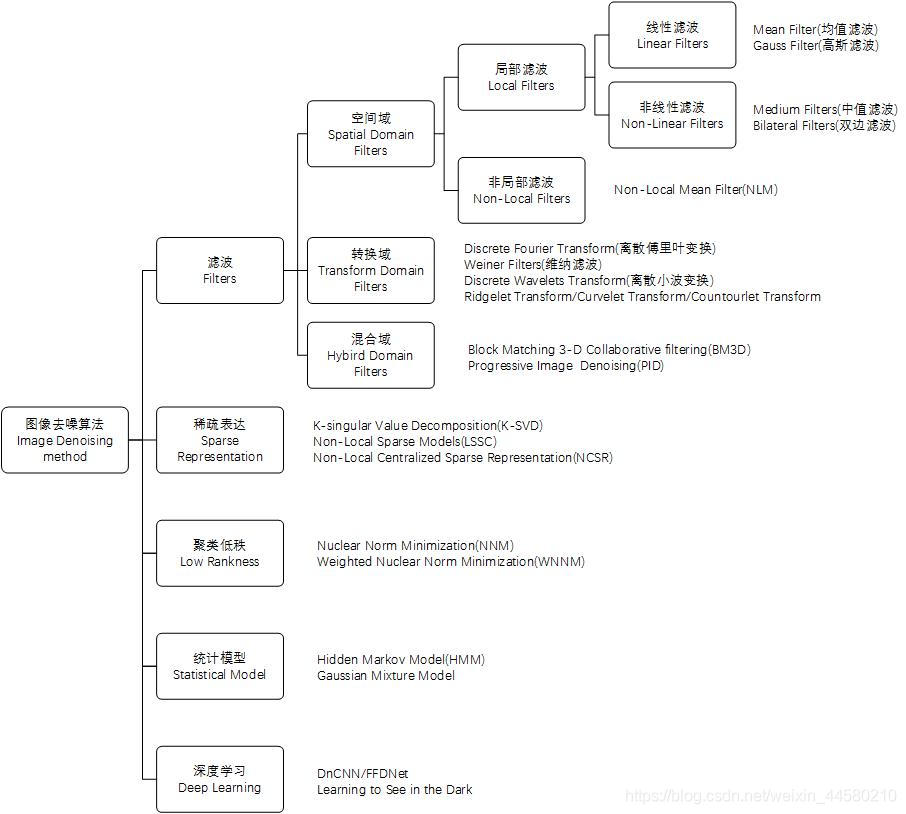
\includegraphics[width=0.8\textwidth]{denoise.jpg}
  \caption{图像降噪算法分类}
  \label{fig:example}
\end{figure}


\section{实验内容}
本次实验一共完成了四项内容:
\begin{itemize}
\item 实现了添加两类噪声的功能,并集成到Moer-lite系统中。
\item 实现了四种传统滤波器降噪方法,并集成到Moer-lite系统中。
\item 集成Intel Open Image Denoise降噪库到Moer-lite系统中。
\item 对比不同滤波器的优缺点和过滤不同噪声的性能。
\end{itemize}

\subsection{修改Moer-lite框架}\label{sec:modify-moer-lite}。%后文需要链接到这里
在Moer-lite框架中,为了实现加噪声、去噪的功能,需要修改框架代码,主要修改部分如下:
\begin{itemize}
\item 在More-lite中,创建一个Noise类用于添加噪声,代码如下: 
\begin{lstlisting}[language=c++]
//FunctionLayer/Noise/Noise.h
#pragma once
#include <ResourceLayer/Image.h>
#include <memory>
#include <vector>

// 实现增加噪声
class Noise {
public:
  //参数可以手动修改
  void AddSaltNoise(const std::shared_ptr<Image>& img, int n=500);
  void AddGaussianNoise(const std::shared_ptr<Image>& img, double mu=0, double sigma=25);
};
\end{lstlisting}

\item 在More-lite中,创建一个Filter类集成传统滤波器,代码如下: 
\begin{lstlisting}[language=c++]
//FunctionLayer/Filter/Filter.h
#pragma once
#include <ResourceLayer/Image.h>
#include <memory>
#include <vector>

// 实现传统滤波器
class Filter {
public:
  //参数可以手动修改
  void MedianFilter(const std::shared_ptr<Image>& src, std::shared_ptr<Image>& dst,double size=3);
  void MeanFilter(const std::shared_ptr<Image>& src,std::shared_ptr<Image>& dst,double size=3);
  void GaussianFilter(const std::shared_ptr<Image>& src, std::shared_ptr<Image>& dst,double size=23, double sigma=0.8);
  std::vector<std::vector<double>> GaussianTemplate(double size, double sigma);
  void BilateralFilter(const std::shared_ptr<Image>& src, std::shared_ptr<Image>& dst, int size=3, float sigmaD=10, float sigmaR=35);
  std::vector<float> RangeTemplate(int range, float sigmaR);
};
\end{lstlisting}

\item 在Film类中调用Filter类和Noise类,添加存储降噪后图片的功能,代码如下:
\begin{lstlisting}[language=c++]
//FunctionLayer/Film/Film.h
#pragma once
#include <CoreLayer/ColorSpace/Spectrum.h>
#include <ResourceLayer/Image.h>
#include <ResourceLayer/JsonUtil.h>
#include <FunctionLayer/Filter/Filter.h>
#include <FunctionLayer/Noise/Noise.h>

class Film {
public:
  Film() = delete;
  Film(const Json &json) {
    size = fetchRequired<Vector2i>(json, "size");
    image = std::make_shared<Image>(size);
    deimage = std::make_shared<Image>(size);
  }

  void deposit(const Vector2i xy, const Spectrum &spectrum) {
    //* 无论光谱内部实现如何,写入图片时均转为3通道格式
    Vector3f v = toVec3(spectrum);
    image->setValue(xy, v);
  }

  void savePNG(const char *filename) { image->savePNG(filename); }
  void saveHDR(const char *filename) { image->saveHDR(filename); } 
  void savePFM(const char *filename) { image->savePFM(filename); }

  //滤波
  void filter(const int type){
    if(type==1) Filter().MedianFilter(image,deimage);
    
    if(type==2) Filter().MeanFilter(image,deimage);

    if(type==3) Filter().GaussianFilter(image,deimage);

    if(type==4) Filter().BilateralFilter(image,deimage);  
  }

  //加噪声
  void addNoise(const int type){
    if(type==1) Noise().AddSaltNoise(image);
    
    if(type==2) Noise().AddGaussianNoise(image); 
  }

  //存储滤波后的图片
  void save_dePNG(const char *filename) { deimage->savePNG(filename); }
  void save_deHDR(const char *filename) { deimage->saveHDR(filename); }

public:
  Vector2i size;

protected:
  std::shared_ptr<Image> image = nullptr;
  std::shared_ptr<Image> deimage = nullptr; //降噪后的image
};
\end{lstlisting}

\item 修改main.cpp文件,在完成渲染后,调用Film类中的加噪声函数和滤波函数,并进行耗时统计,添加的代码如下:
\begin{lstlisting}[language=c++]
//main.cpp
//main函数最后增加对含有三个参数的命令的判断:
  //需要加噪声/滤波
  if (argc == 4 ) {
    // 命令格式为“./Moer <样例路径> <加噪声> <去噪>”
    const std::string noise = std::string(argv[2]); // 获取第三个参数的值,噪声类型
    const std::string denoise = std::string(argv[3]); // 获取第四个参数的值,去噪类型
    //存储加噪声的图片
    std::string outputName1 = fetchRequired<std::string>(json["output"], "filename");
    std::size_t extensionPos1 = outputName.find_last_of(".");
    //存储去噪的图片
    std::string outputName2 = fetchRequired<std::string>(json["output"], "filename");
    std::size_t extensionPos2 = outputName.find_last_of(".");
    
    //加噪声
    printf("\n********Begin Add Noise********\n");
    //加椒盐噪声
    if(noise=="add_salt_noise") {
      camera->film->addNoise(1);
      if (extensionPos1 != std::string::npos) {
        outputName1.insert(extensionPos1, "_add_salt_noise");
      }
    }
    //加高斯噪声
    else if(noise=="add_g_noise") {
      camera->film->addNoise(2);
      if (extensionPos1 != std::string::npos) {
        outputName1.insert(extensionPos1, "_add_g_noise");
      }
    }
    //不加噪声
    else if(noise=="none") {
        
    }
    else {
      std::cout<<"Only support add_salt_noise, add_g_noise, none\n";
    }

    //存储加过噪声的图片
    if (std::regex_match(outputName1, std::regex("(.*)(\\.png)"))) {
      camera->film->savePNG(outputName1.c_str());
    } else if (std::regex_match(outputName1, std::regex("(.*)(\\.hdr)"))) {
      camera->film->saveHDR(outputName1.c_str());
    } else {
      std::cout << "Only support output as PNG/HDR\n";
    }

    std::cout<< "Save noise image to "<<outputName1<<std::endl;

    //去噪
    auto s = std::chrono::system_clock::now();
    auto e = std::chrono::system_clock::now();;
    printf("\n********Begin Denoise********\n");
    //中值去噪
    if(denoise=="median_denoise") {
      camera->film->filter(1);
      e = std::chrono::system_clock::now();
      if (extensionPos2 != std::string::npos) {
        outputName2.insert(extensionPos2, "_median_denoise");
      }
    }
    //均值去噪
    else if(denoise=="mean_denoise") {
      camera->film->filter(2);
      e = std::chrono::system_clock::now();
      if (extensionPos2 != std::string::npos) {
        outputName2.insert(extensionPos2, "_mean_denoise");
      }
    }
    //高斯去噪
    else if(denoise=="g_denoise") {
      camera->film->filter(3);
      e = std::chrono::system_clock::now();
      if (extensionPos2 != std::string::npos) {
        outputName2.insert(extensionPos2, "_g_denoise");
      }
    }
    //双边去噪
    else if(denoise=="bi_denoise") {
      camera->film->filter(4);
      e = std::chrono::system_clock::now();
      if (extensionPos2 != std::string::npos) {
        outputName2.insert(extensionPos2, "_bi_denoise");
      }
    }
    //Intel降噪库去噪
     else if(denoise=="intel_denoise") {
        //构造输入pfm图片
        camera->film->savePFM("tmp.pfm");
        //执行Intel降噪库的sh命令
        const char* command = "./oidnDenoise -hdr tmp.pfm -o re.pfm"; 
        // 使用system函数执行Shell命令
        system(command); 
        e = std::chrono::system_clock::now();
         std::cout<< "Save denoised image to re.pfm"<<std::endl;
        printf("\nIntel Denoising costs %.2fs\n",(std::chrono::duration_cast<std::chrono::milliseconds>(e - s)) .count() / 1000.f);
        return 0; 
    }
    //不去噪声
    else if(denoise=="none") {
       printf("\nIntel Denoising costs %.2fs\n",(std::chrono::duration_cast<std::chrono::milliseconds>(e - s)) .count() / 1000.f);
       return 0;
    }
    else {
      std::cout<<"Only support median_denoise, mean_denoise, g_denoise, bi_denoise, intel_denoise, none\n";
    }

    //输出降噪后的图片
    if (std::regex_match(outputName2, std::regex("(.*)(\\.png)"))) {
      camera->film->save_dePNG(outputName2.c_str());
    } else if (std::regex_match(outputName2, std::regex("(.*)(\\.hdr)"))) {
      camera->film->save_deHDR(outputName2.c_str());
    } else {
      std::cout << "Only support output as PNG/HDR\n";
    }

    std::cout<< "Save denoised image to "<<outputName2<<std::endl;
    // 计算去噪用时
    printf("\nIntel Denoising costs %.2fs\n",(std::chrono::duration_cast<std::chrono::milliseconds>(e - s)) .count() / 1000.f);   
  }
\end{lstlisting}

\item 增加执行Moer命令的参数,调用main.cpp中的相应代码
\begin{lstlisting}[language=c++]
//1. 不进行滤波和降噪,只传入一个参数
./Moer <场景描述文件的目录>

//2. 进行滤波/降噪,需要传入三个参数
./Moer <场景描述文件的目录> <add_salt_noise/add_g_noise/none> <mean_denoise/median_denoise/g_denoise/bi_denoise/none>
\end{lstlisting}

\end{itemize}
\subsection{图像噪声模型}
在降噪前,先对不同的图像噪声进行建模,以便对比同一滤波器对不同噪声的滤波效果。本次实验中主要实现椒盐噪声和高斯噪声的建模。

图像降噪模型可以建模为:
\begin{equation}\label{eu_eqn}
y=x+n
\end{equation}
其中,$y$是观察到的噪声图像,$x$是图像真值,$n$是图像噪声,图像降噪过程就是通过$y$获取$x$,在许多论文中将这个过程描述为不可逆过程\cite{gu2019review},这也就是为什么图像降噪难度较大。

\subsubsection{高斯噪声}\label{sec:g_noise}%后文需要链接到这里
\textcolor{third}{\textbf{1. 定义:}}

高斯噪声是最常见也是最重要的的一种噪声,众多的图像降噪算法都以降低高斯噪声为目标设计,其概率密度函数为
\begin{equation}\label{eu_eqn}
p(z)=\frac{1}{\sqrt{2\pi\sigma^2}}e^{-(z-\mu)^2}/2\sigma^2
\end{equation}
其中,$\sigma$是标准偏差,$\mu$是灰度值的平均值,这个公式说明的是灰度值为$z$的概率为多少。

\textcolor{third}{\textbf{2. 代码思路:}}

随机生成两个随机数,利用Box-Muller公式将两个均匀分布的随机数转换为服从均值为$\mu$,标准差为$\sigma$ 的高斯分布的随机数,并且控制添加噪声的数据范围,使之适合降噪\cite{zhihu97905713}。在数据范围内给像素点加上符合高斯分布的值。

\textcolor{third}{\textbf{3. 代码集成:}}

在More-lite中,集成生成高斯噪声的代码如下:
\begin{lstlisting}[language=c++]
//FunctionLayer/Noise/Noise.cpp
// 添加高斯噪声
void Noise::AddGaussianNoise(const std::shared_ptr<Image>& img, double mu, double sigma) 
{
    int width = img->size[0];
    int height = img->size[1];
    int channels = Image::channels;

    int RandomArray[width+1][height+1];
    for (int i = 0; i < width; i++) {
        for (int j = 0; j <height; j++) {
			RandomArray[i][j] = (rand() % (255 - 0 + 1)) + 0;
			//要取得[a,b)的随机整数,使用(rand() % (b-a))+ a;   			
			//要取得[a,b]的随机整数,使用(rand() % (b-a+1))+ a;   			
			//要取得(a,b]的随机整数,使用(rand() % (b-a))+ a + 1;   		
		    }
	    }
     //计算要添加噪声的数据范围小于20%
     int down1 = 0, up1 = 255 * 1 / 20;//0-0.05

    for (int i = 0; i < width; i++) {
        for (int j = 0; j < height; j++) {
            if (RandomArray[i][j]<up1&&RandomArray[i][j]>down1){
                Vector2i xy(i, j);            
                if (channels == 1) {  //只有一个通道,是灰度图
                    // 构建高斯噪声
                    double u1, u2;
                    do {
                        u1 = rand() * (1.0 / RAND_MAX);
                        u2 = rand() * (1.0 / RAND_MAX);
                    } while (u1 <= std::numeric_limits<double>::min()); // u1不能为0

                    double z = sigma * sqrt(-2.0 * log(u1)) * cos(2 * PI * u2) + mu;

                    Vector3f pixelVal = img->getValue(xy);
                    int val = static_cast<int>(pixelVal[0] + z * 32);
                    val = (val < 0) ? 0 : val;
                    val = (val > 255) ? 255 : val;

                    Vector3f newPixelVal(val, val, val);
                    img->setValue(xy, newPixelVal);
                } else { //多个通道,是彩色图
        
                    for (int k = 0; k < channels; k++) {
                        // 构建高斯噪声
                        //产生随机数
                        double u1, u2;
                        do {
                            u1 = rand() * (1.0 / RAND_MAX);
                            u2 = rand() * (1.0 / RAND_MAX);
                        } while (u1 <= std::numeric_limits<double>::min()); // u1不能为0

                        //利用 Box-Muller 公式将两个均匀分布的随机数转换为服从均值为 mu,标准差为 sigma 的高斯分布的随机数 z
                        double z = sigma * sqrt(-2.0 * log(u1)) * cos(2 * PI * u2) + mu;

                        Vector3f pixelVal = img->getValue(xy);
                        
                        int val = static_cast<int>(pixelVal[k] + z*32);
                        val = (val < 0) ? 0 : val;
                        val = (val > 255) ? 255 : val;

                        pixelVal[k] = val;
                        img->setValue(xy, pixelVal);
                    }
                }
            }
        }
    }   
}
\end{lstlisting}

\subsubsection{椒盐噪声}
\textcolor{third}{\textbf{1. 定义:}}

椒盐噪声又称脉冲噪声、尖峰噪声,在图像上表现为随机分布的黑白点,其概率密度函数为
\begin{equation}\label{eu_eqn}
p(z)=
\begin{cases}
P_a, & z=a \\
P_b, & z=b \\
1-P_a-P_b, & otherwise
\end{cases}
\end{equation}

椒盐噪声可以通过中值滤波器进行消除。

\textcolor{third}{\textbf{2. 代码思路:}}

在代码中利用一个变量n来控制添加的椒盐噪声的数量。各生成n个黑点和n个白点随机分布。

\textcolor{third}{\textbf{2. 代码集成:}}

在More-lite中,集成生成椒盐噪声的代码如下:
\begin{lstlisting}[language=c++]
//FunctionLayer/Noise/Noise.cpp
// 添加椒盐噪声
void Noise::AddSaltNoise(const std::shared_ptr<Image>& img, int n) {
    int width = img->size[0];
    int height = img->size[1];

    for (int k = 0; k < n; k++) {
        int x = rand() % width;
        int y = rand() % height;

        Vector3f whitePixel(255, 255, 255); // White color

        img->setValue(Vector2i(x, y), whitePixel);
    }

    for (int k = 0; k < n; k++) {
        int x = rand() % width;
        int y = rand() % height;

        Vector3f blackPixel(0, 0, 0); // Black color

        img->setValue(Vector2i(x, y), blackPixel);
    }
}
\end{lstlisting}



\subsection{传统滤波器降噪}
空间域滤波器可以分为局部滤波器和非局部滤波器,其中局部滤波器又分为线性滤波器和非线性滤波器。经典的局部滤波器如中值滤波、均值滤波、高斯滤波、双边滤波,其中均值滤波和高斯滤波为线性滤波器,中值滤波和双边滤波为非线性滤波。




\subsubsection{中值滤波}
\textcolor{third}{\textbf{1. 定义:}}

如图~\ref{fig:s1}所示,以目标像素周围$3 \times 3$的邻域为例,就是将$3 \times 3$邻域中九个像素灰度值进行排序,将中间灰度值作为目标像素的灰度值。由于椒盐噪声影响的像素的灰度值通常都非常大或者非常小,因此通过排序会被消除掉。

相比于其他三种传统滤波器,中值滤波的特点有三:
\begin{itemize}
 \item 没有引入新的像素值
 \item 有利于消除脉冲噪声、椒盐噪声
 \item 保边
\end{itemize}

\textcolor{third}{\textbf{2. 代码思路:}}

\begin{itemize}
\item 传入的参数:保存原图的Image对象、保存输出图的Image对象、窗口大小(默认为3)。

\item 图片边缘处理:一般来说,在对图像应用滤波器进行过滤时,边界问题是一个需要处理的问题。有3种处理的方法,如图\ref{fig:boundary}所示。
    \begin{itemize}
    \item 不做边界处理
不对图像的边界作任何处理,在对图像进行滤波时,滤波器没有作用到图像的四周,因此图像的四周没有发生改变。
    \item 填充0
对图像的边界做扩展,在扩展边界中填充0,对于边长为2k+1的方形滤波器,扩展的边界大小为k,若原来的图像为[m, n],则扩展后图像变为[m+2k, n+2k]。进行滤波之后,图像会出现一条黑色的边框。
    \item 填充最近像素值
扩展与 填充0 的扩展类似,只不过填充0的扩展是在扩展部分填充0,而这个方法是填充距离最近的像素的值。
    \end{itemize}

\textcolor{main}{\textbf{注:在本实验中,所有滤波都采取对边缘填充0的策略。}}

\item 求中值:通过遍历窗口中的所有像素值并进行排序,得到中值。

\end{itemize}

\begin{figure}
    \centering
    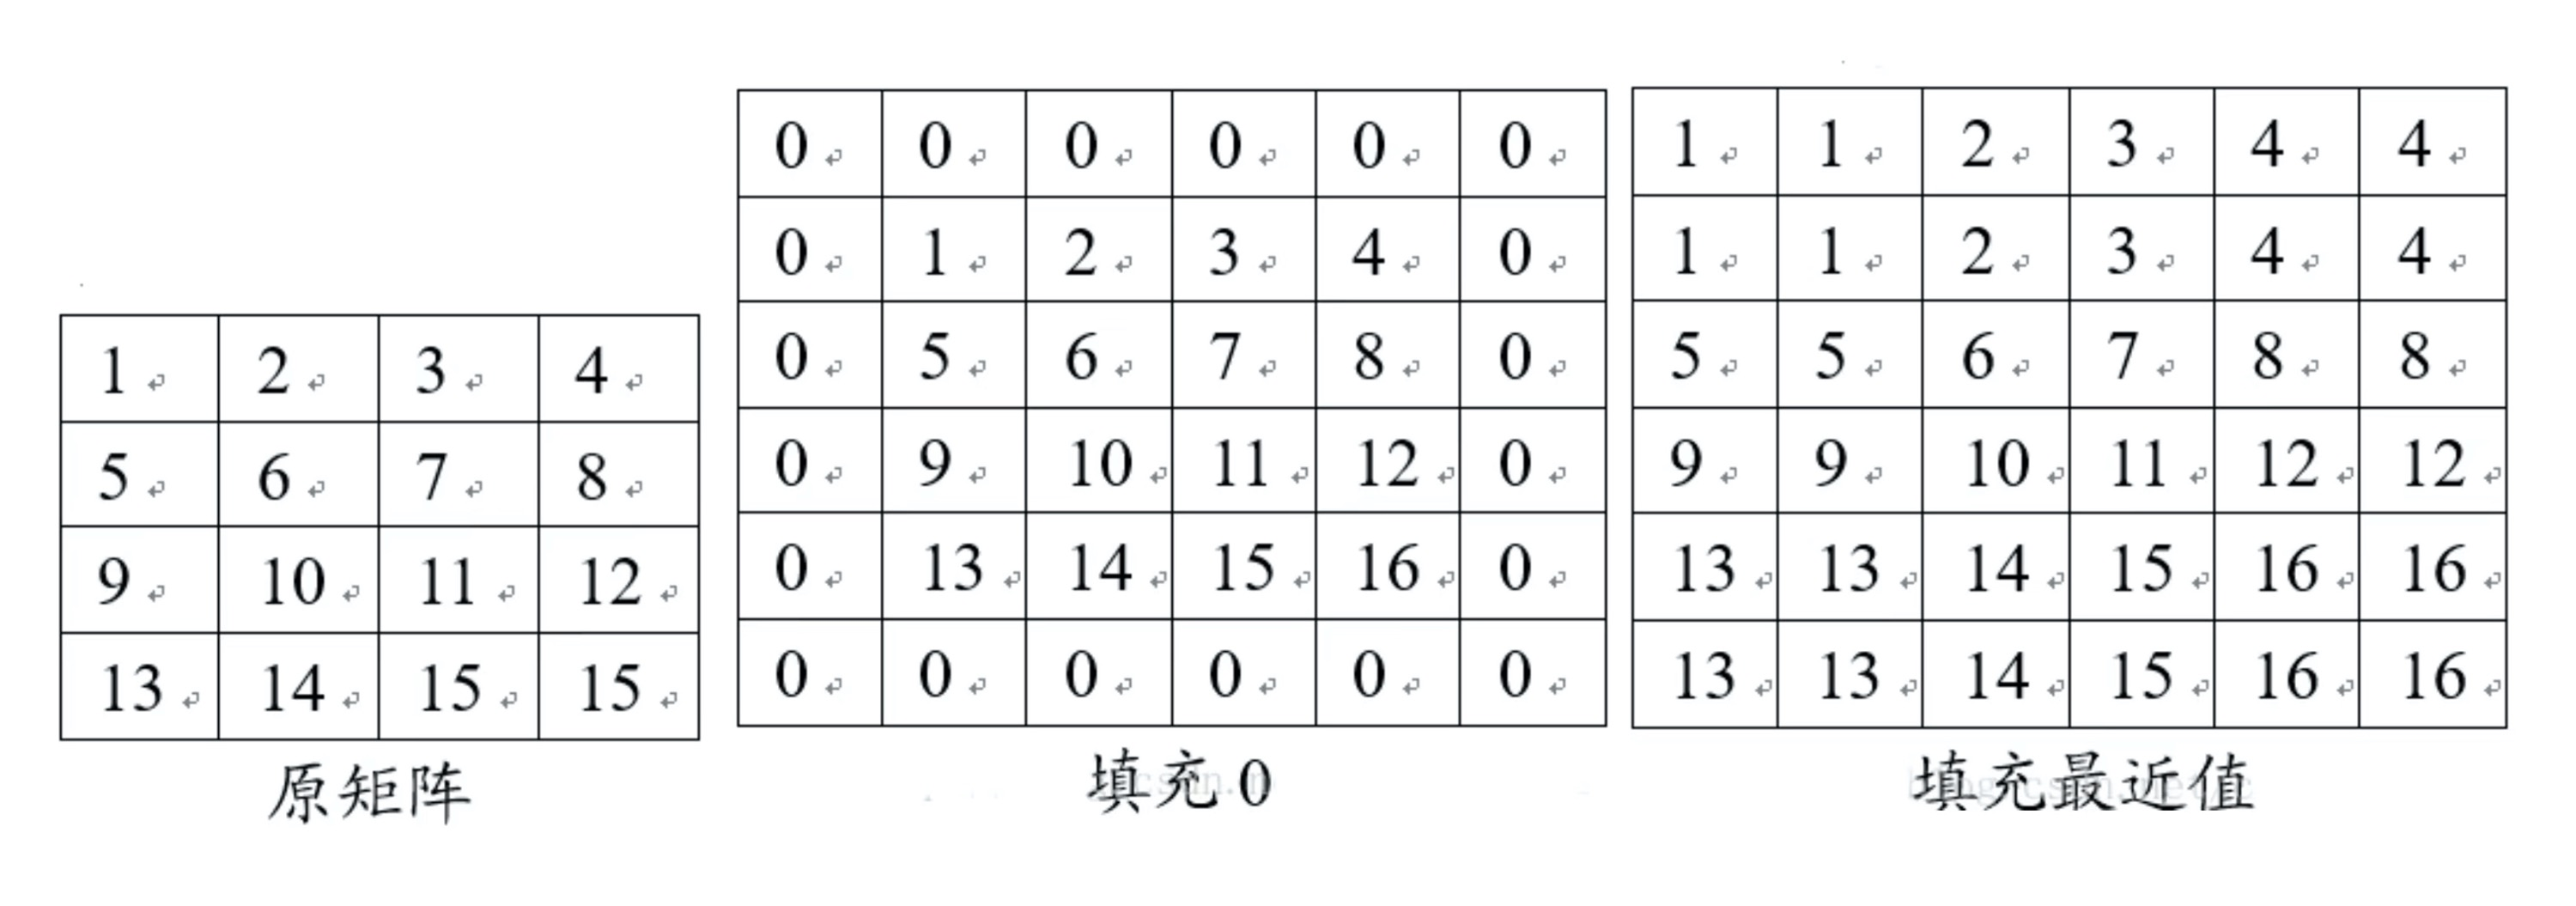
\includegraphics[width=.8\textwidth]{boundary.png}
    \caption{边缘处理的三种方式}
    \label{fig:boundary}
\end{figure}



\textcolor{third}{\textbf{3. 代码集成:}}

在More-lite中,集成中值滤波的代码如下: 
\begin{lstlisting}[language=c++]
//FunctionLayer/Filter/Filter.cpp
// 中值滤波
void  Filter::MedianFilter(const std::shared_ptr<Image>& src, std::shared_ptr<Image>& dst,double size)
{
     //边缘像素默认填充0
    int start = size / 2;
    for (int i = start; i < dst->size[1] - start; i++)
    {
        for (int j = start; j < dst->size[0] - start; j++)
        {
            // 收集邻域内的像素值
            std::vector<Vector3f> model;
            for (int m = i - start; m <= i + start; m++)
            {
                for (int n = j - start; n <= j + start; n++)
                {
                    model.push_back(src->getValue(Vector2i(n, m)));
                }
            }
            // 对邻域内的像素值进行排序
           std::sort(model.begin(), model.end(), [](const Vector3f& a, const Vector3f& b) {
            return a.length() < b.length();
            });

            // 取中值作为输出图像中的像素值
            dst->setValue(Vector2i(j, i), Vector3f(model[size * size / 2]));
        }
    }
}
\end{lstlisting}

\begin{figure}
  \centering

  \subfigure[中值滤波原理]{
    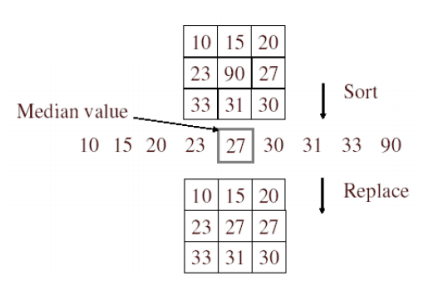
\includegraphics[width=0.45\textwidth]{median.png}
    \label{fig:s1}
  }
  \hfill
  \subfigure[中值滤波与均值滤波对比]{
    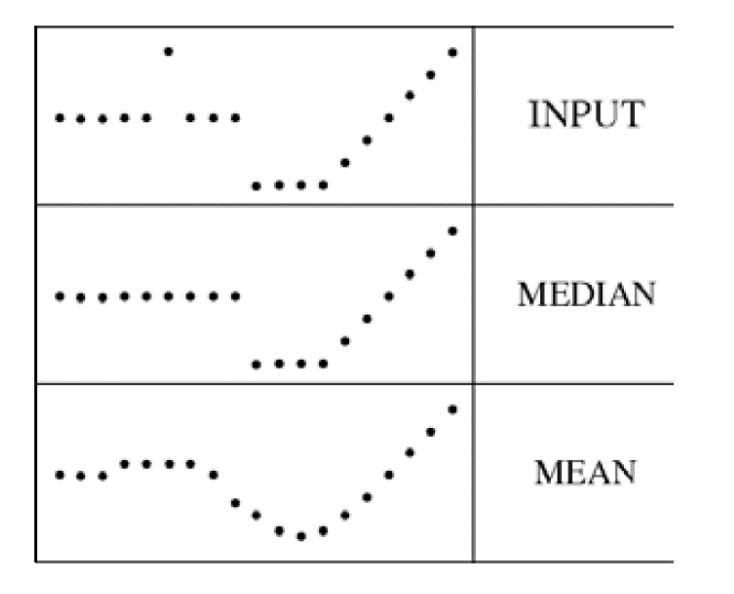
\includegraphics[width=0.45\textwidth]{com.png}
    \label{fig:s2}
  }

  \caption{中值滤波与均值滤波}
  \label{fig:me}
\end{figure}

\subsubsection{均值滤波}
\textcolor{third}{\textbf{1. 定义:}}
同样以目标像素周围$3\times 3$的邻域为例,就是将$3\times 3$邻域中九个像素灰度值的平均值作为目标像素的灰度值。

如图~\ref{fig:s2}所示,相比于中值滤波,均值滤波会模糊边缘。但是均值滤波耗时较少。

\textcolor{third}{\textbf{2. 代码思路:}}

代码思路与中值滤波相似,通过控制窗口大小,求窗口中所有像素值的均值赋予中间像素。

\textcolor{third}{\textbf{3. 代码集成:}}

在More-lite中,集成均值滤波的代码如下:
\begin{lstlisting}[language=c++]
//FunctionLayer/Filter/Filter.cpp
// 均值滤波
void Filter::MeanFilter(const std::shared_ptr<Image>& src,std::shared_ptr<Image>& dst, double size)
{
    int start = size / 2;
    for (int i = start; i < dst->size[1] - start; i++)
    {
        for (int j = start; j < dst->size[0] - start; j++)
        {
            Vector3f sum(0.0f, 0.0f, 0.0f);
            for (int m = i - start; m <= i + start; m++)
            {
                for (int n = j - start; n <= j + start; n++)
                {
                    Vector3f value = src->getValue(Vector2i(n, m));
                    sum += value;
                }
            }
            Vector3f average = sum / (size * size);
            dst->setValue(Vector2i(j, i), average);
        }
    } 
}
\end{lstlisting}



\subsubsection{高斯滤波}
\textcolor{third}{\textbf{1. 定义:}}

高斯滤波器是一种线性滤波器,其作用原理和均值滤波器类似,都是取滤波器窗口内的像素的均值作为输出。其窗口模板的系数和均值滤波器不同,均值滤波器的模板系数都是相同的为1;而高斯滤波器的模板系数随着距离模板中心的增大而系数减小。所以,高斯滤波器相比于均值滤波器对图像个模糊程度较小。

高斯滤波主要可以使用两种方法实现。一种是离散化窗口滑窗卷积,另一种方法是通过傅里叶变化。只有当离散化的窗口非常大,用滑窗计算量非常大的情况下,会考虑基于傅里叶变化的实现方法。本次试验中选择使用滑窗实现的卷积。

离散化窗口滑窗卷积时主要利用大小为奇数的高斯核,常用的高斯模板的计算公式为
\begin{equation}\label{eu_eqn}
G(x,y)\frac{1}{2\pi\sigma^2}e^{-\frac{x^2+y^2}{2\sigma^2}}
\end{equation}

这样输出的模板有两种形式:
\begin{itemize}
 \item 小数类型:直接计算得到的值,没有经过任何处理。

 \item 整数类型:将得到的值进行归一化处理,即将左上角的值归一化为1,其他每个系数都除以左上角的系数,然后取整。在使用整数模板时,需要在模板的前面加一个系数,该系数为模板系数之和的倒数。
\end{itemize}

\textcolor{third}{\textbf{2. 参数理解:}}

影响高斯滤波器效果的参数有两个,一是核(kernel)的取值,即窗口的大小,二是$\sigma$的取值。如图~\ref{fig:twosubfigures}所示,图~\ref{fig:subfig1}展示了相同大小的$\sigma$,不同大小的kernel对高斯滤波的影响,表明kernel的尺寸越大,越完整,但是计算开销越大;图~\ref{fig:subfig2}展示了相同大小的kernel,不同大小的$\sigma$对高斯滤波的影响。标准差代表着数据的离散程度,若$\sigma$较小,则生成的模板的中心系数较大,周围的系数较小,图像的平滑效果不明显;反之,$\sigma$较大,则生成的模板的各个系数相差不大,与均值模板类似,对图像的平滑效果更明显。


\begin{figure}
  \centering

  \subfigure[相同大小的$\sigma$,不同大小的kernel]{
    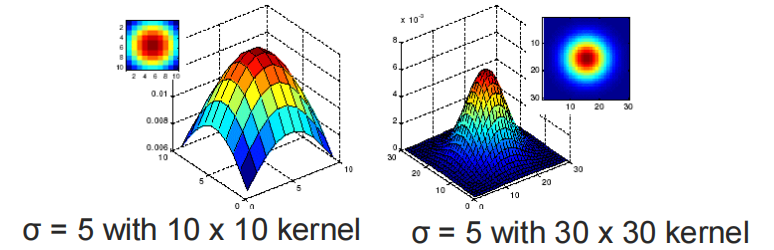
\includegraphics[width=0.45\textwidth]{g1.png}
    \label{fig:subfig1}
  }
  \hfill
  \subfigure[相同大小的kernel,不同大小的$\sigma$]{
    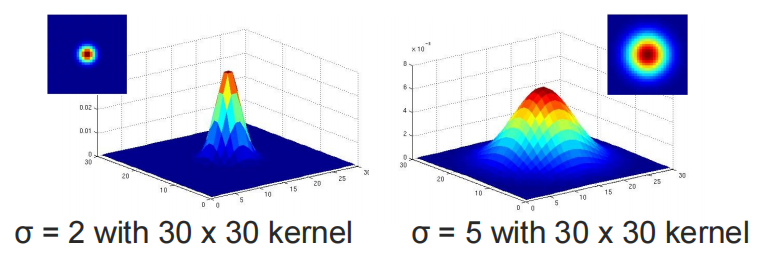
\includegraphics[width=0.45\textwidth]{g2.png}
    \label{fig:subfig2}
  }

  \caption{高斯滤波的影响因素。一是核(kernel)的大小,二是$\sigma$的取值。kernel的尺寸越大,越完整,但是计算开销越大;标准差代表着数据的离散程度,若$\sigma$较小,则生成的模板的中心系数较大,周围的系数较小,图像的平滑效果不明显;反之,$\sigma$较大,则生成的模板的各个系数相差不大,与均值模板类似,对图像的平滑效果更明显。}
  \label{fig:twosubfigures}
\end{figure}

\textcolor{third}{\textbf{3. 代码思路:}}

在窗口数组中遍历,使用单独的高斯模版计算函数求得高斯掩模的值,作为权重与数组相乘。核中间的像素值为加权和。

实际上,高斯掩膜的求解与位置(x,y)无关,因为在计算过程中x,y被抵消掉了,因此只要计算一次就可以了。

%\vspace{12pt}
\textcolor{third}{\textbf{4. 代码集成:}}

在More-lite中,集成高斯滤波的代码如下:
\begin{lstlisting}[language=c++]
//FunctionLayer/Filter/Filter.cpp
// 高斯滤波
void Filter::GaussianFilter(const std::shared_ptr<Image>& src, std::shared_ptr<Image>& dst,double size, double sigma)
{
    std::vector<std::vector<double>> gaussianTemplate = GaussianTemplate(size,sigma);
    int start = size / 2;
    for (int i = start; i < dst->size[1] - start; i++)
    {
        for (int j = start; j < dst->size[0] - start; j++)
        {
            Vector3f sum(0.0f, 0.0f, 0.0f);
            for (int m = i - start; m <= i + start; m++)
            {
                for (int n = j - start; n <= j + start; n++)
                {
                    Vector3f value = src->getValue(Vector2i(n, m));
                    float weight = gaussianTemplate[m - i + start][n - j + start];
                    sum += value * weight;
                }
            }
            dst->setValue(Vector2i(j, i), sum);
        }
    } 
}

//高斯掩膜的求解与位置(x,y)无关,因为在计算过程中x,y被抵消掉了,因此只要计算一次就可以了
//需要size,sigma
//同时也是双边滤波的空间域模版
std::vector<std::vector<double>> Filter::GaussianTemplate(double size, double sigma)
{
    std::vector<std::vector<double>> temp;
    double base = 1.0 / 2.0 / PI / sigma / sigma;
    for(int i = 0; i < size; i++)
    {
        std::vector<double> vec;
        for(int j = 0; j < size; j++)
        {
            double a = (pow(i - size/2, 2) + pow(j - size/2, 2)) / 2.0 / sigma / sigma;
            double b = base * exp(-a);
            vec.push_back(b);
        }
        temp.push_back(vec);
    }
    return temp;
}
\end{lstlisting}


\subsubsection{双边滤波}
\textcolor{third}{\textbf{1. 定义:}}

高斯滤波去降噪,会较明显地模糊边缘,对于高频细节的保护效果并不明显,因此引入双边滤波。双边滤波(Bilateral filter)是一种非线性的滤波方法,是结合图像的空间邻近度和像素值相似度的一种折衷处理,同时考虑空域信息和灰度相似性,达到保边去噪的目的,如图~\ref{fig:bi}所示。双边滤波器比高斯滤波多了一个高斯方差,它是基于空间分布的高斯滤波函数,所以在边缘附近,离的较远的像素不会太多影响到边缘上的像素值,这样就保证了边缘附近像素值的保存。但是由于保存了过多的高频信息,对于彩色图像里的高频噪声,双边滤波器不能够干净的滤掉,只能够对于低频信息进行较好的滤波。

\begin{figure}
  \centering
  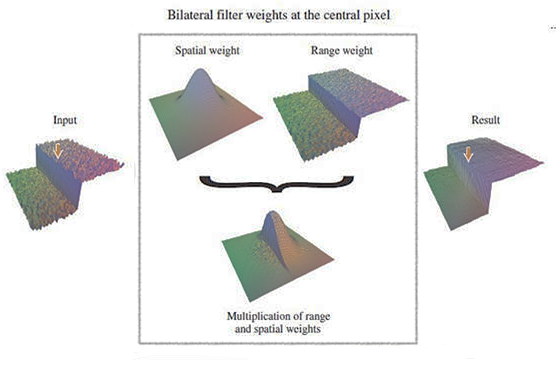
\includegraphics[width=0.8\textwidth]{bi.png}
  \caption{双边滤波示意图}
  \label{fig:bi}
\end{figure}

双边滤波器的核由两个函数生成:空间域核和值域核。
\begin{itemize}

\item 空间域核:由像素位置欧式距离决定的模板权值$w_d$:
\begin{equation}\label{eu_eqn}
w_d(i,j,k,l)=e^{-\frac{(i-k)^2+(j-l)^2}{2\sigma_d^2}}
\end{equation}
其中,$q(i,j)$为模板窗口的其他系数的坐标;$p(k,l)$为模板窗口的中心坐标点;$\sigma_d$为高斯函数的标准差。 使用该公式生成的滤波器模板和高斯滤波器使用的模板是没有区别的。

 \item 值域核:由像素值的差值决定的模板权值$w_r$:
 \begin{equation}\label{eu_eqn}
w_r(i,j,k,l)=e^{-\frac{\Vert f(i,j)-f(k,l) \Vert^2}{2\sigma_r^2}}
\end{equation}
其中,$q(i,j)$为模板窗口的其他系数的坐标,$f(i,j)$表示图像在点$q(i,j)$处的像素值;$p(k,l)$为模板窗口的中心坐标点,对应的像素值为$f(k,l)$, $\sigma_r$为高斯函数的标准差。

\end{itemize}

将上述两个模板相乘就得到了双边滤波器的模板权值:
\begin{equation}\label{eu_eqn}
w(i,j,k,l)=w_d(i,j,k,l)*w_r(i,j,k,l)=e^{-\frac{(i-k)^2+(j-l)^2}{2\sigma_d^2}-\frac{\Vert f(i,j)-f(k,l) \Vert^2}{2\sigma_r^2}}
\end{equation}

因此,双边滤波器的数据公式可以表示如下:
\begin{equation}\label{eu_eqn}
g(i,j)=\frac{\sum_{k,l}f(k,l)w(i,j,k,l)}{\sum_{k,l}w(i,j,k,l)}
\end{equation}

\textcolor{third}{\textbf{2. 参数理解:}}

空域权重$w_d$衡量的是$p,q$两点之间的距离,距离越远权重越低;值域权重$w_r$衡量的是$p,q$两点之间的像素值相似程度,越相似权重越大。

从图像的平坦区域和边缘区域定性分析双边滤波的降噪效果:在平坦区域,临近像素的像素值的差值较小,对应值域权重$w_r$接近于1,此时空域权重$w_d$起主要作用,相当于直接对此区域进行高斯模糊。因此,平坦区域相当于进行高斯模糊;在边缘区域,临近像素的像素值的差值较大,对应值域权重$w_r$接近于0,导致此处核函数下降(因$w=w_r∗w_d$),当前像素受到的影响就越小,从而保持了原始图像的边缘的细节信息。

\textcolor{third}{\textbf{3. 代码思路:}}

与高斯滤波相似,在窗口数组中遍历,使用单独的空间域模板(高斯模板)计算函数求得高斯掩模的值,使用单独的值域模板计算函数求得值域掩模的值,两值相乘作为权重与数组相乘。核中间的像素值为加权和。

\textcolor{third}{\textbf{4. 代码集成:}}

在More-lite中,集成高斯滤波的代码如下:
\begin{lstlisting}[language=c++]
//FunctionLayer/Filter/Filter.cpp
// 双边滤波,去噪保边
void Filter::BilateralFilter(const std::shared_ptr<Image>& src, std::shared_ptr<Image>& dst, int size, float sigmaD, float sigmaR)
{
    std::vector<std::vector<double>> spatialTemplate = GaussianTemplate(size, sigmaD);
    std::vector<float> rangeTemplate = RangeTemplate(256, sigmaR);

    int start = size / 2;

    for (int y = start; y < src->size[1] - start; ++y)
    {
        for (int x = start; x < src->size[0] - start; ++x)
        {
            Vector3f sum(0.0f, 0.0f, 0.0f);
            float weightSum = 0.0f;

            for (int i = y - start; i <= y + start; ++i)
            {
                for (int j = x - start; j <= x + start; ++j)
                {
                    Vector3f value = src->getValue(Vector2i(j, i));
                    float spatialWeight = spatialTemplate[i - y + start][j - x + start];
                    float rangeWeight = rangeTemplate[static_cast<int>(std::abs(value.length()))];
                    float weight = spatialWeight * rangeWeight;

                    sum += value * weight;
                    weightSum += weight;
                }
            }
            dst->setValue(Vector2i(x, y), sum / weightSum);
        }
    }
}
//空间域模版使用高斯模版
//值域模版
std::vector<float> Filter::RangeTemplate(int range,float sigmaR)
{
    std::vector<float> mask;
    float base = 1.0f / (2.0f * sigmaR * sigmaR);

    for (int i = 0; i < range; ++i)
    {
        float distance = i * i;
        float weight = std::exp(-distance / (2.0f * sigmaR * sigmaR));
        mask.push_back(weight);
    }

    return mask;
}
\end{lstlisting}


\subsection{Intel Open Image Denoise工业降噪库}
\textcolor{third}{\textbf{1. 介绍:}}

英特尔开放图像去噪库\cite{oidn_website}的核心是一系列基于高效深度学习的去噪滤波器,这些滤波器经过训练可以处理各种spp样本。因此它适用于预览和最终帧渲染。过滤器可以仅使用带噪声的color缓冲区对图像进行去噪,也可以为了保留尽可能多的细节,选择使用辅助特征缓冲区(例如反照率、法线)。

\textcolor{third}{\textbf{2. 代码集成:}}
\begin{itemize}
\item 参考Open Image Denoise的GitHub仓库\cite{oidn_github}中的步骤,下载源码并编译,获得bin、include、lib文件,将得到的这三个文件夹复制合并到Moer-lite编译后生成的target文件夹中,如图~\ref{fig:oidfigures}所示。

\begin{figure}[htp] %优先放在当前位置
\centering
  \subfigure[Step1: 编译open image denoise源文件]{
    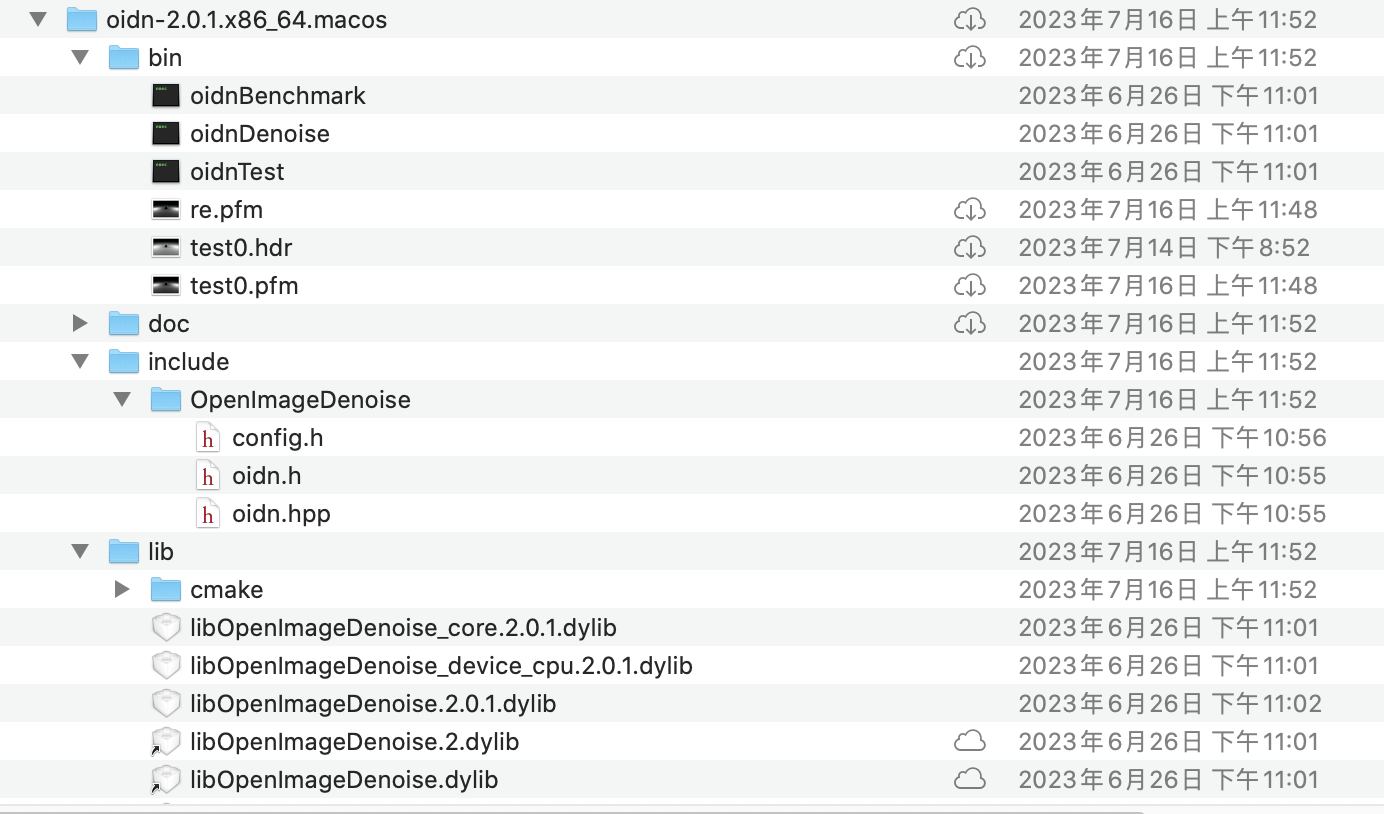
\includegraphics[width=0.45\textwidth]{oid1.png}
    \label{fig:oid1}
  }
  \hfill
  \subfigure[Step2: 复制合并到Moer-lite编译后生成的target文件夹中]{
    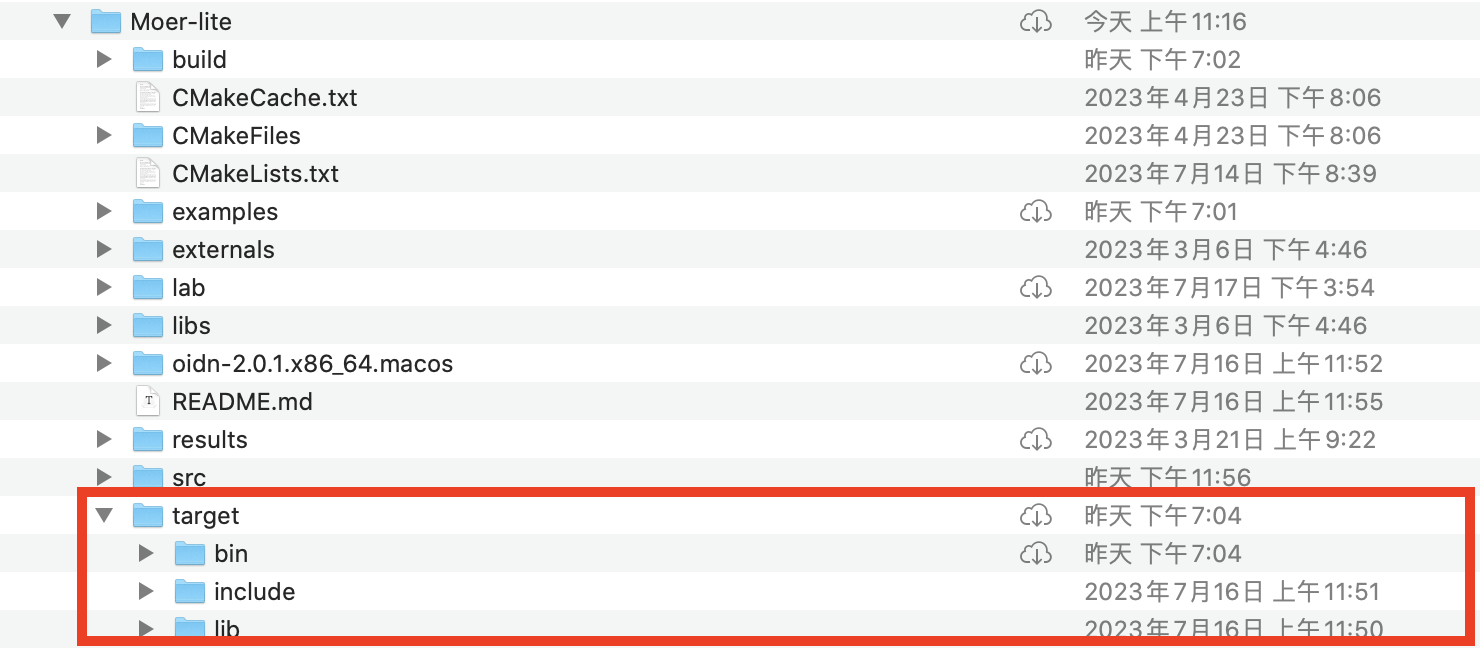
\includegraphics[width=0.45\textwidth]{oid2.png}
    \label{fig:oid2}
  }

  \caption{Moer-lite集成Intel Open Image Denoise降噪库}
  \label{fig:oidfigures}

\end{figure}

\item 由于降噪库滤波的输入图片需要为pfm格式,因此在Image类中增加Image::savePFM函数:
\begin{lstlisting}[language=c++]
//ResourceLayer/Image.cpp
void Image::savePFM(const char* filename) const {
  std::ofstream f(filename, std::ios::binary);
  if (!f.is_open()) {
    std::cerr << "Failed to open file: " << filename << std::endl;
    return;
  }

  f << "PF\n";
  f << size[0] << " " << size[1] << "\n";
  f << "-1.0\n";

  for (int y = size[1] - 1; y >= 0; --y) {
    for (int x = 0; x < size[0]; ++x) {
      const int offset = (x + y * size[0]) * channels;
      for (int c = 0; c < channels; ++c) {
        const float value = data[offset + c];
        f.write(reinterpret_cast<const char*>(&value), sizeof(float));
      }
    }
  }

  f.close();
}
\end{lstlisting}

\item Intel Open Image Denoise降噪库的执行命令为
\texttt{./oidnDenoise -hdr <输入图片路径> -o <输出图片路径>},需要在Moer-lite代码中执行过程中执行这一行shell命令,集成结果参见\hyperref[sec:modify-moer-lite]{1.3.1 修改Moer-lite框架}一节。

\item 增加执行Moer命令的参数,调用main.cpp中的相应代码。集成结果参见\hyperref[sec:modify-moer-lite]{1.3.1 修改Moer-lite框架}一节。

\end{itemize}

\section{实验结果与分析}

\textcolor{main}{\textbf{注:由于Latex不支持hdr格式的图片导入,所以实验报告所有出现的图片均为截图,截图的方式也许会导致图片边缘不完全准确,但是尽量对准了边缘进行截图并放在实验报告中。}}

\subsection{添加噪声}

\begin{enumerate}[itemsep=1.5ex]
  \item 椒盐噪声
  
\quad 分别设置噪声点个数为500、2000、10000,添加噪声后结果如下:

\begin{figure}[htbp]
	\centering
	\subfigure[原图]{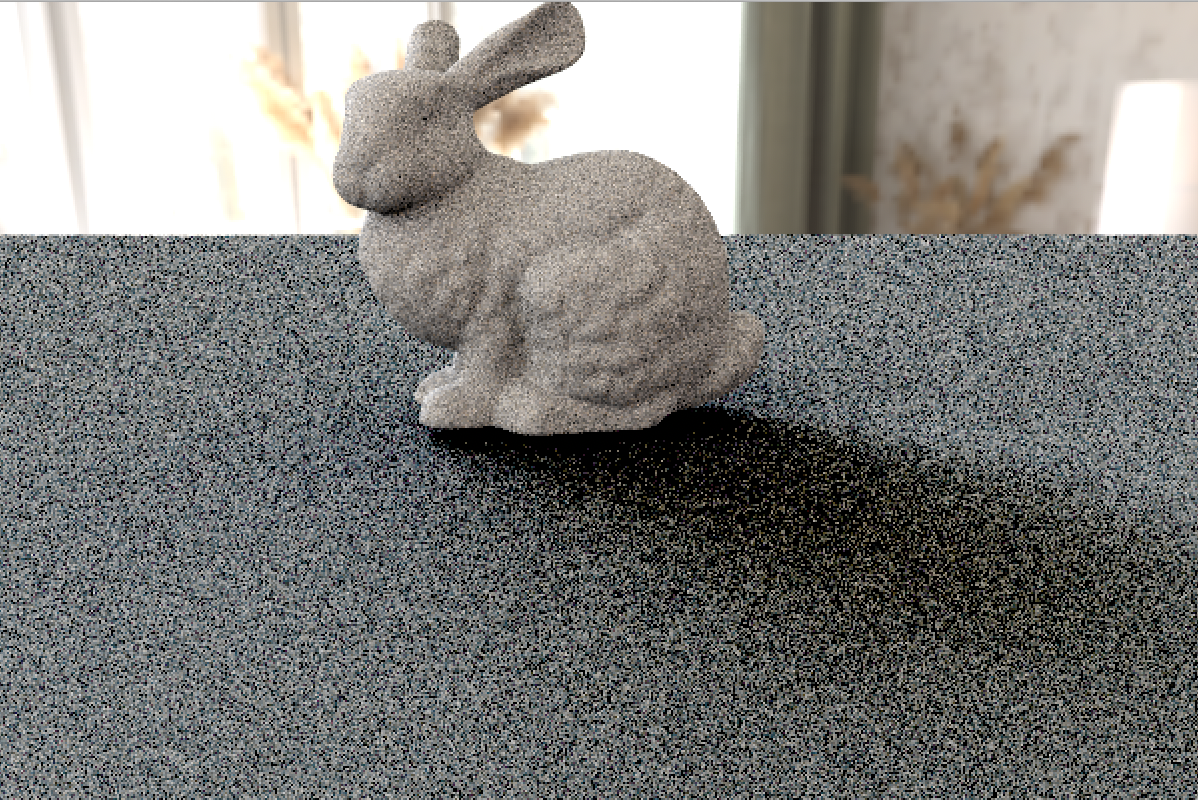
\includegraphics[width=.2\textwidth]{salt.png}}
	\subfigure[添加500个噪声点] {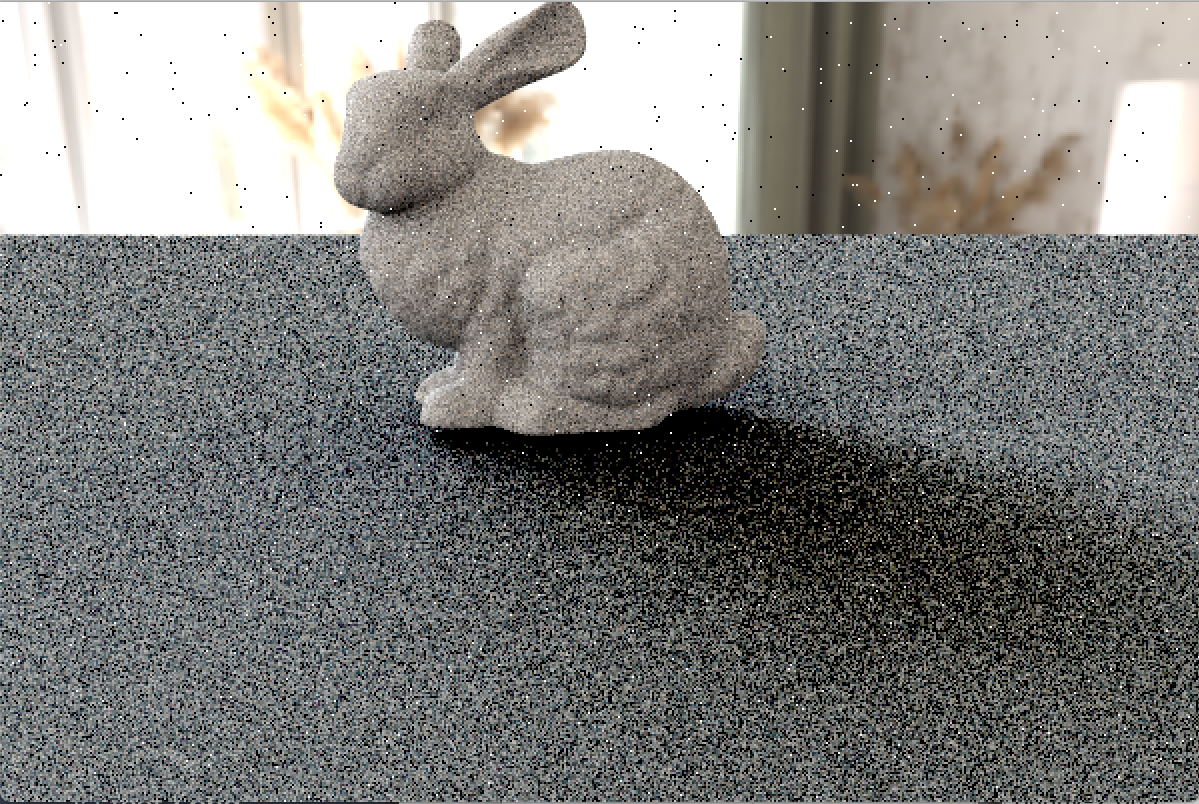
\includegraphics[width=.2\textwidth]{salt500.png}}
	\subfigure[添加2000个噪声点] {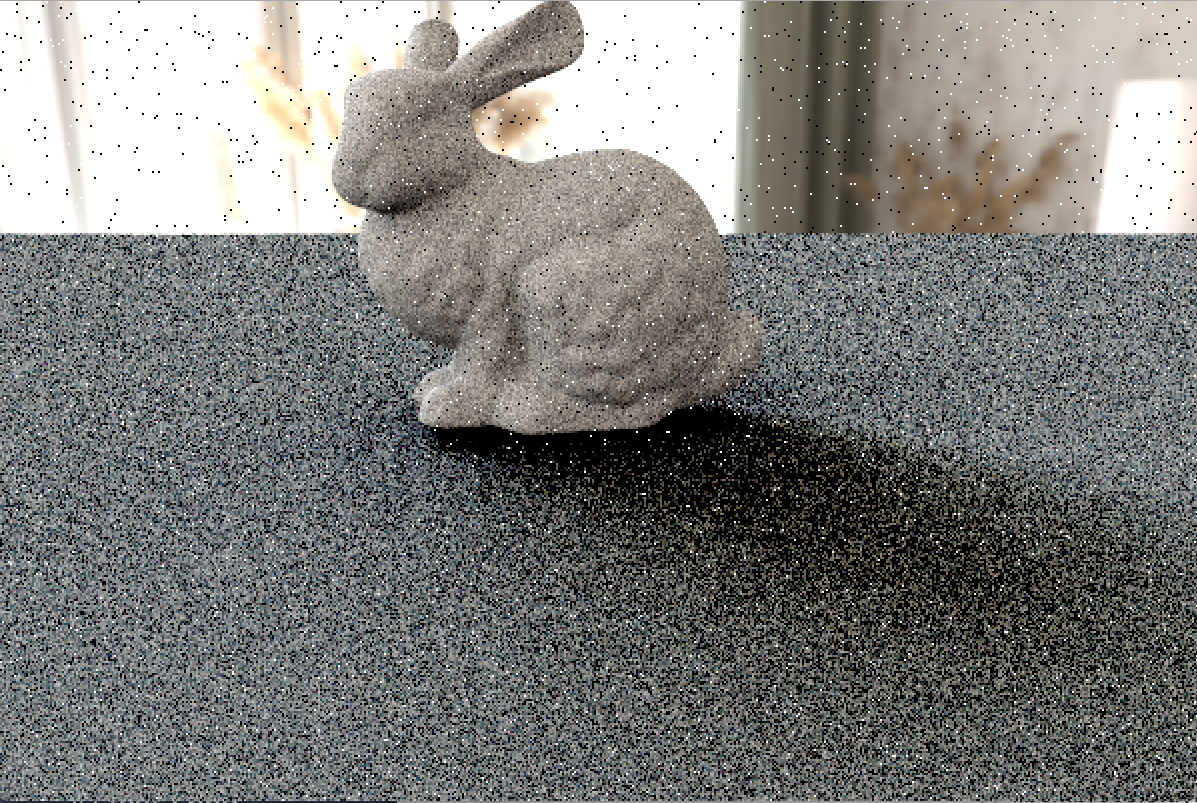
\includegraphics[width=.2\textwidth]{salt2000.png}}
    \subfigure[添加10000个噪声点] {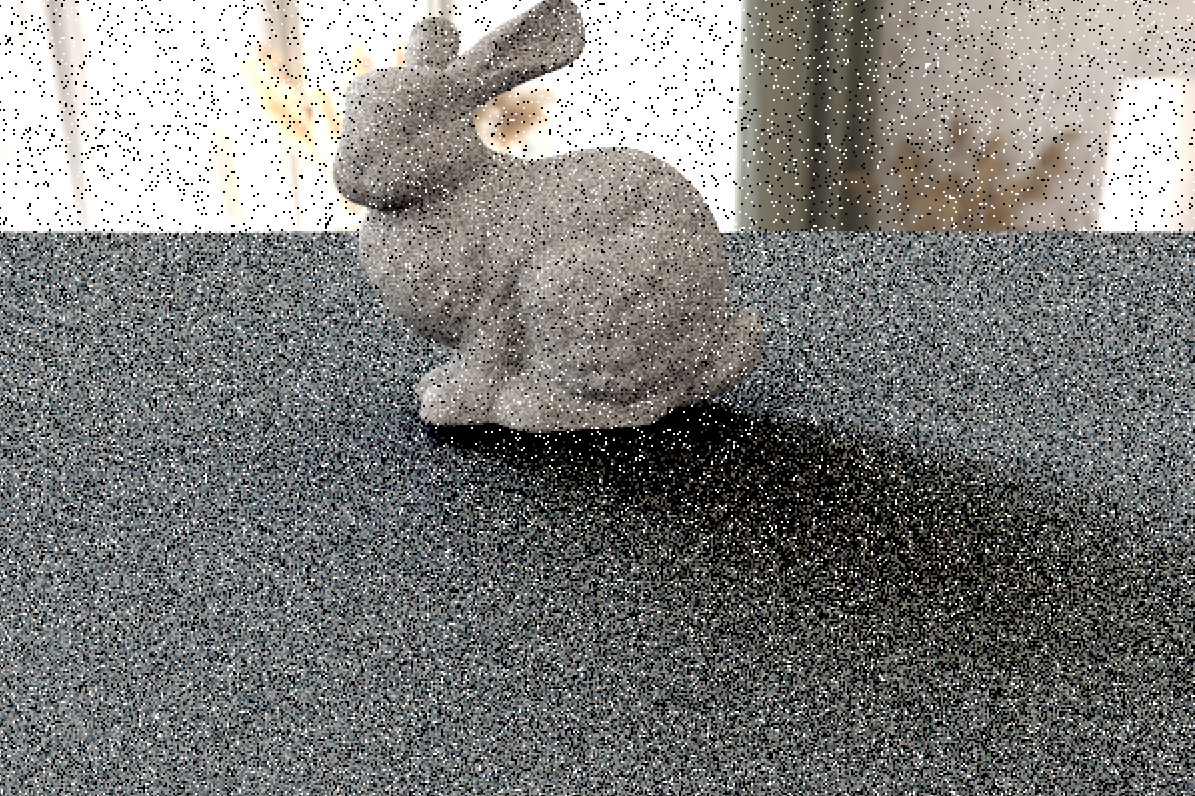
\includegraphics[width=.2\textwidth]{salt10000.png}}
	\caption{添加椒盐噪声}
	\label{salt_noise}
\end{figure}

\quad \textcolor{second}{\textbf{分析:}}显而易见,噪声点n值越大,图片上的黑白噪点越多。

\item 高斯噪声

\quad 生成高斯噪声的函数主要由两个变量需要控制(参见\hyperref[sec:g_noise]{1.3.2.1 高斯噪声}一节),一是要添加噪声的数据范围,二是$\sigma$,$\mu$默认为0。

\quad 分别设置不同的参数值,添加噪声后结果如~\ref{fig:g_noise}所示。
\begin{figure}[htbp]
	\centering
	\subfigure[原图]{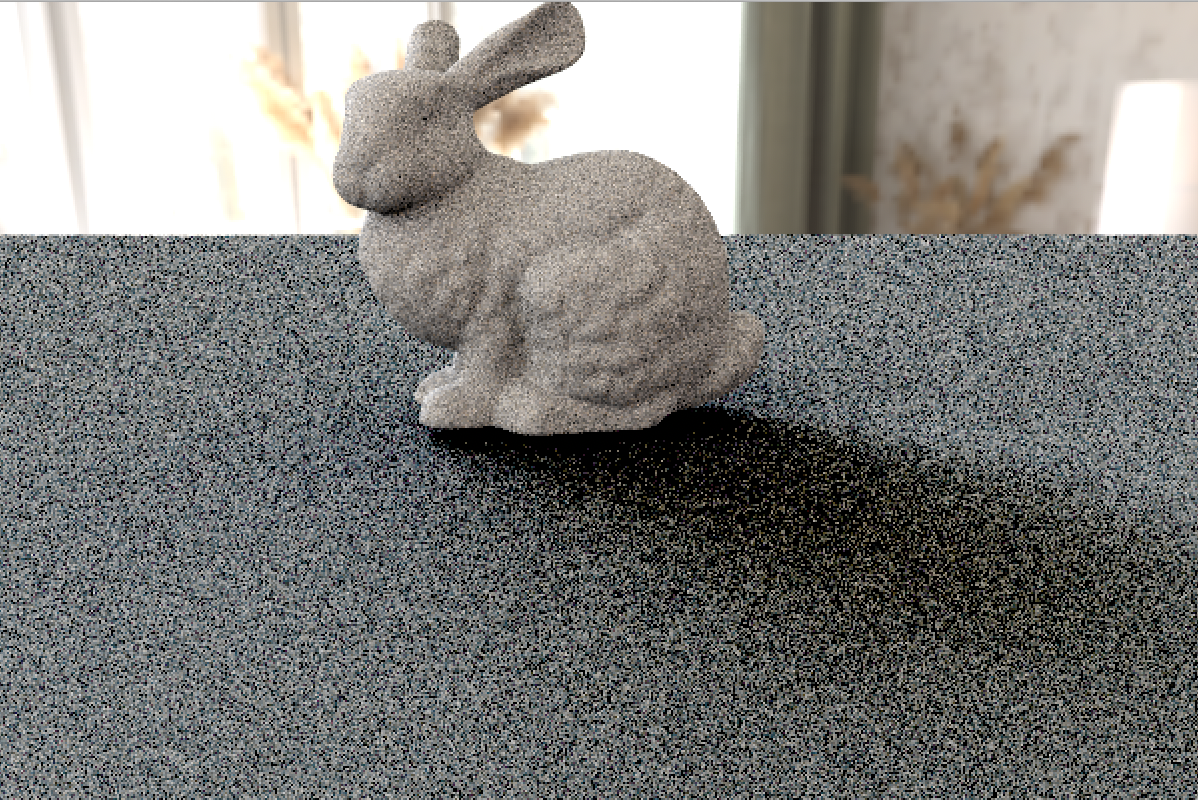
\includegraphics[width=.3\textwidth]{salt.png}}
    \label{fig:salt}
	\subfigure[添加噪声的数据范围为20\%,$\sigma=0.1$] {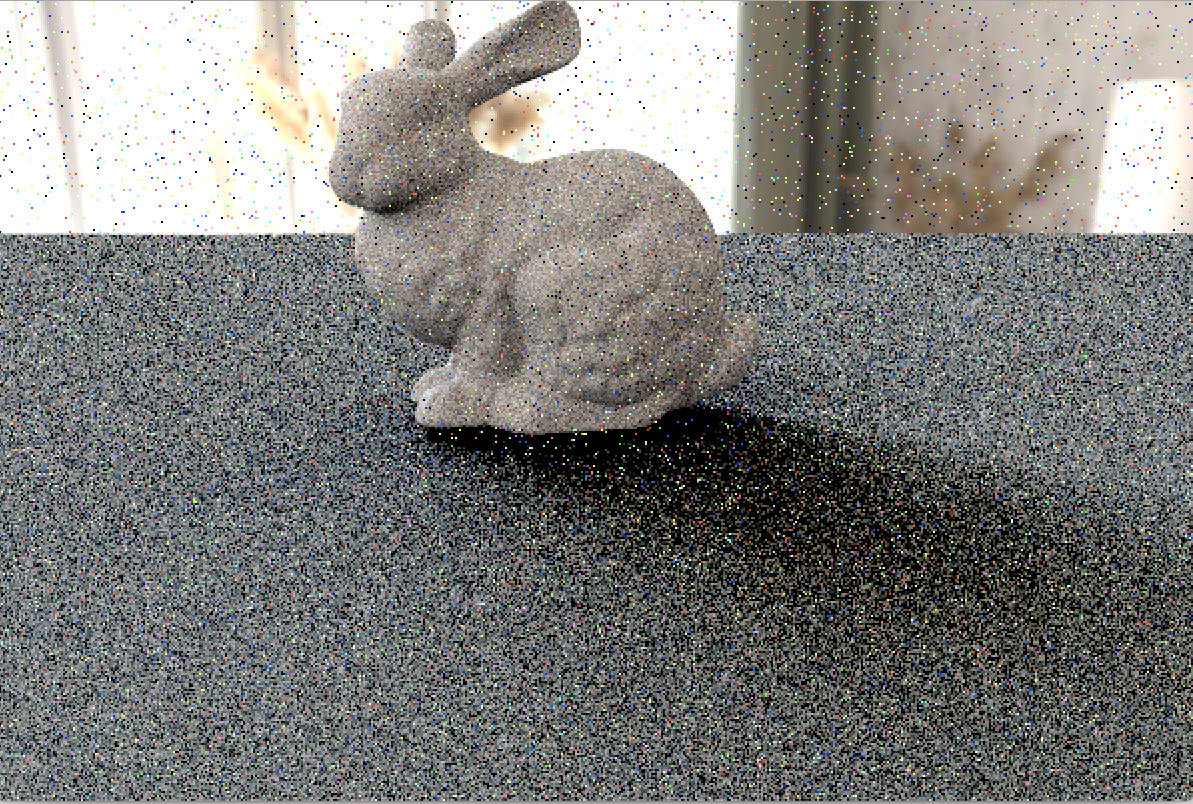
\includegraphics[width=.3\textwidth]{g_0.1.png}}
    \label{fig:g_0.1}
	\subfigure[添加噪声的数据范围为20\%,$\sigma=1$,即正态分布] {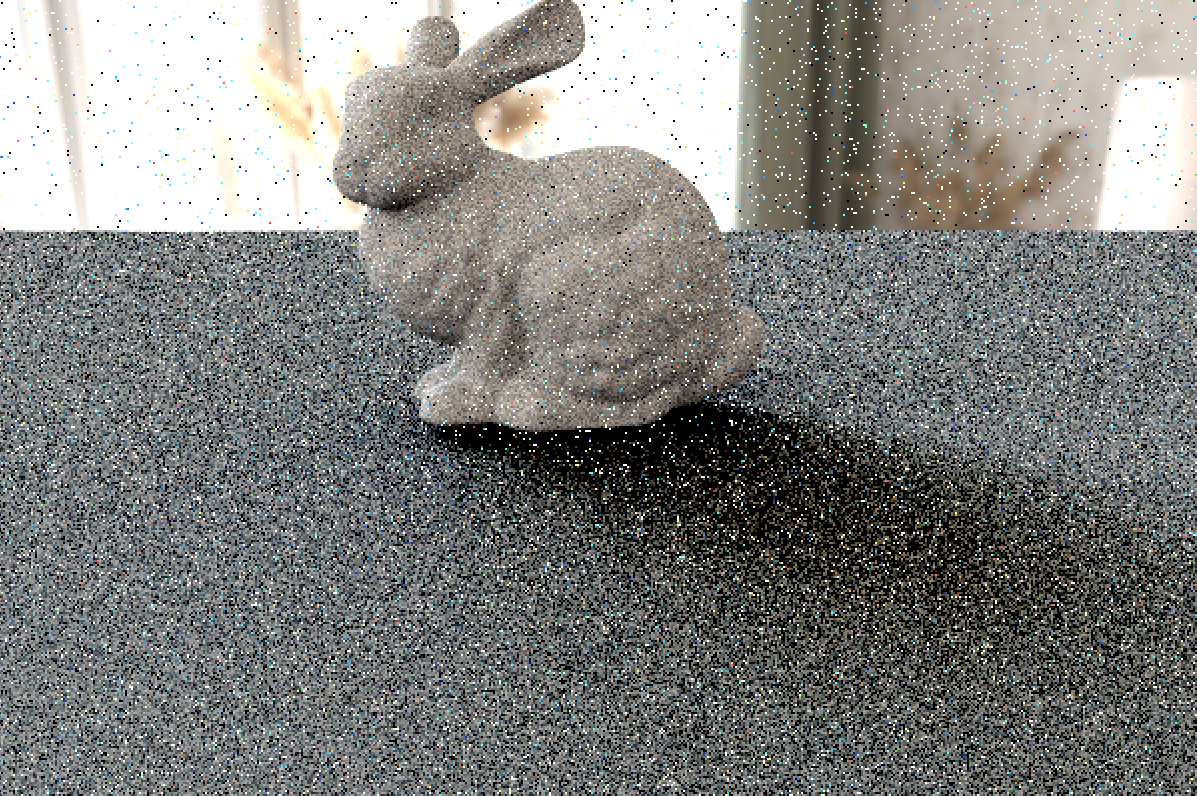
\includegraphics[width=.3\textwidth]{g_1.png}}
    \label{fig:g_1}
    \subfigure[添加噪声的数据范围为20\%,$\sigma=200$] {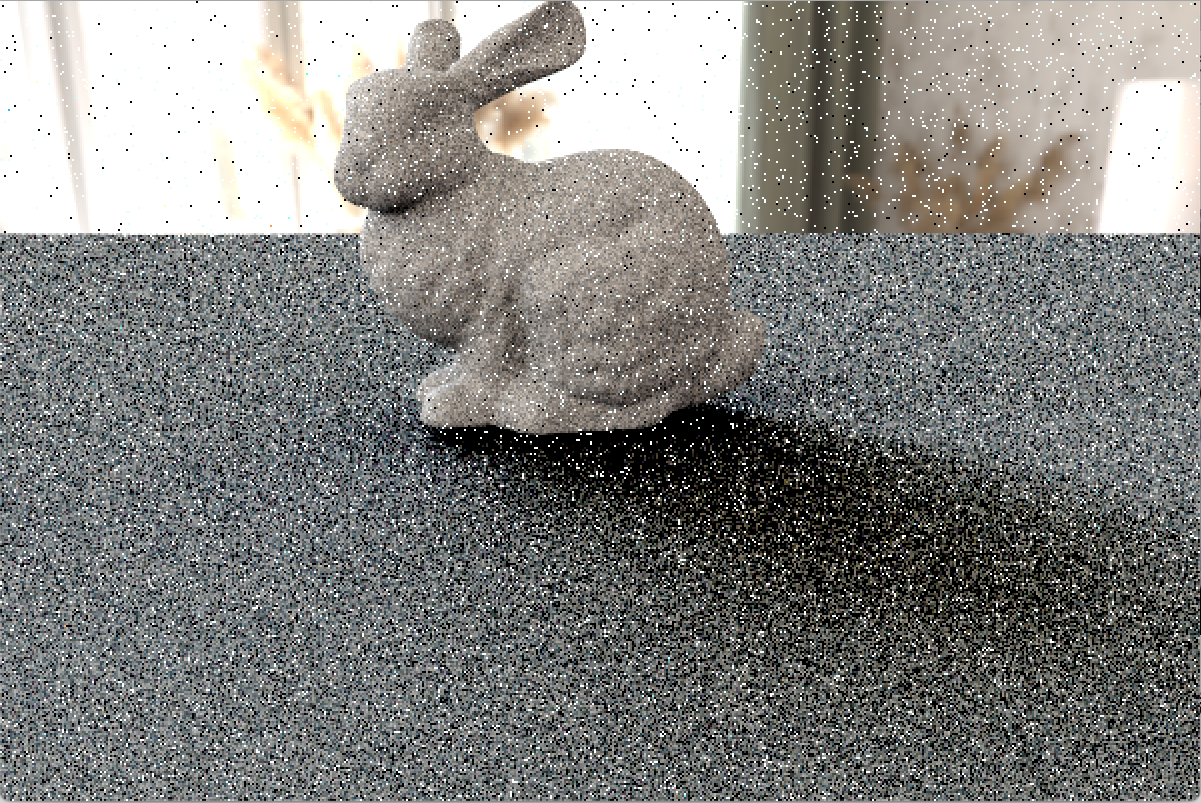
\includegraphics[width=.3\textwidth]{g_200.png}}
    \label{fig:g_200}
    \subfigure[添加噪声的数据范围为50\%,$\sigma=1$]{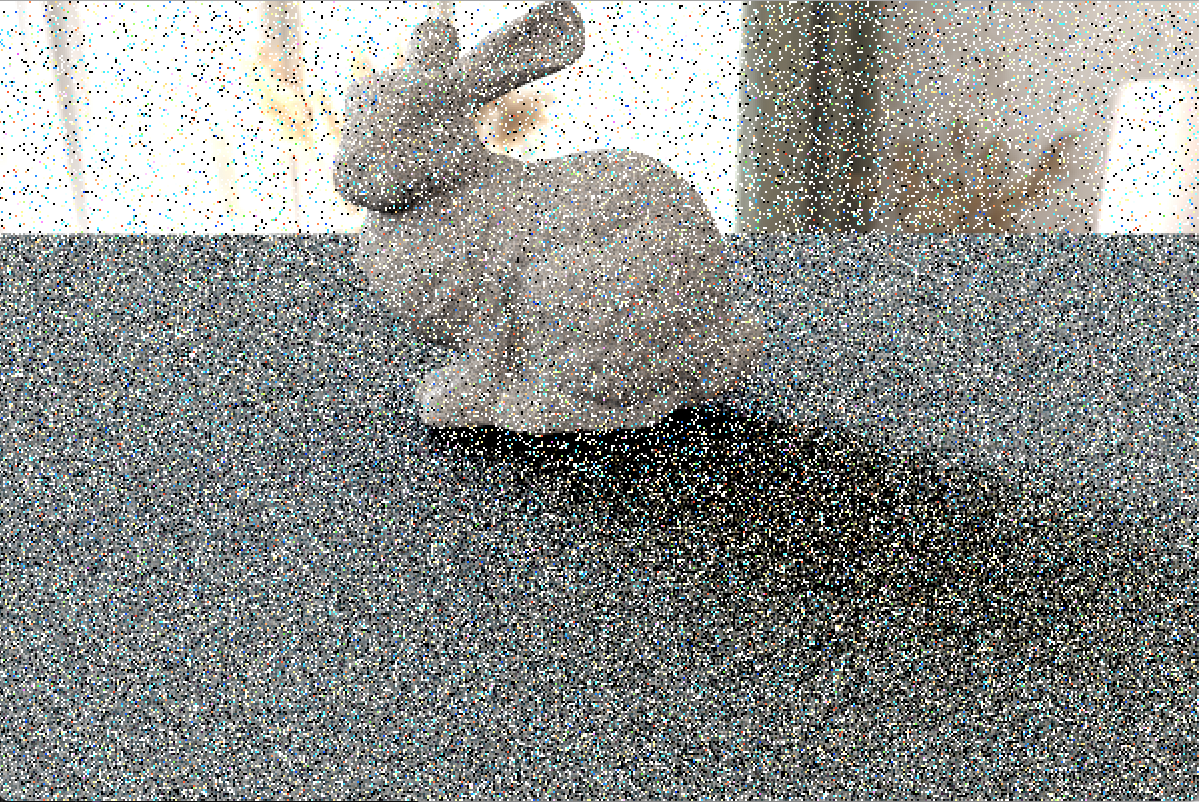
\includegraphics[width=.3\textwidth]{g_50f.png}}
    \label{fig:50f}
    \subfigure[添加噪声的数据范围为100\%,$\sigma=1$]{
\includegraphics[width=.3\textwidth]{g_100f.png}}
    \label{fig:100f}
	\caption{添加高斯噪声}
	\label{fig:g_noise}
\end{figure}

\vspace{12pt}
\quad \textcolor{second}{\textbf{分析:}}
\begin{itemize}
\item 较大的$\sigma$值会生成更强烈的噪声,噪声点与原始像素值的差异更大,使图像中的噪声更加明显。同时,较大的$\sigma $值会使噪声点分布更广泛,图像中的噪声更加扩散和分散。较小的 $\sigma$ 值则会生成集中在均值附近的细小噪声点,使噪声更集中。
\item 需要合理控制添加噪声的数据范围,例如当数据范围为100\%,即RGB值在$[0,255]$之间的像素都需要添加噪声时,就会出现如图1.7(f)所示情况,这种图片不适合用于做降噪。

\end{itemize}

 \end{enumerate}
 
\subsection{中值滤波}
在分析中值滤波的效果时,一共做了四组对比实验:
\vspace{5pt}
\begin{enumerate}[itemsep=1.5ex]

\item 对照组:使用中值滤波过滤未添加噪声的图片。如图~\ref{fig:median_cmp1}所示。

\item 同样大小的窗口对不同程度的椒盐噪声的去噪效果:使用窗口大小为3的中值滤波过滤添加椒盐噪声的图片,n的取值包含500、10000。如图~\ref{fig:median_cmp2.1}和~\ref{fig:median_cmp2.2}所示。

\item 同样大小的窗口对不同程度的高斯噪声的去噪效果:使用窗口大小为3的中值滤波过滤添加高斯噪声的图片,$\sigma$取值包含0.1、1、100,数据处理范围为20\%。如图~\ref{fig:median_cmp3.1}、~\ref{fig:median_cmp3.2}和~\ref{fig:median_cmp3.3}所示。

\item 不同大小的窗口对同样程度的椒盐噪声的去噪效果:使用窗口大小为3、21的中值滤波过滤添加椒盐噪声的图片。如图~\ref{fig:median_cmp2.2}和~\ref{fig:median_cmp4}所示。

\end{enumerate}

\begin{figure}[htbp]
	\centering
	\subfigure[渲染得到的原图]{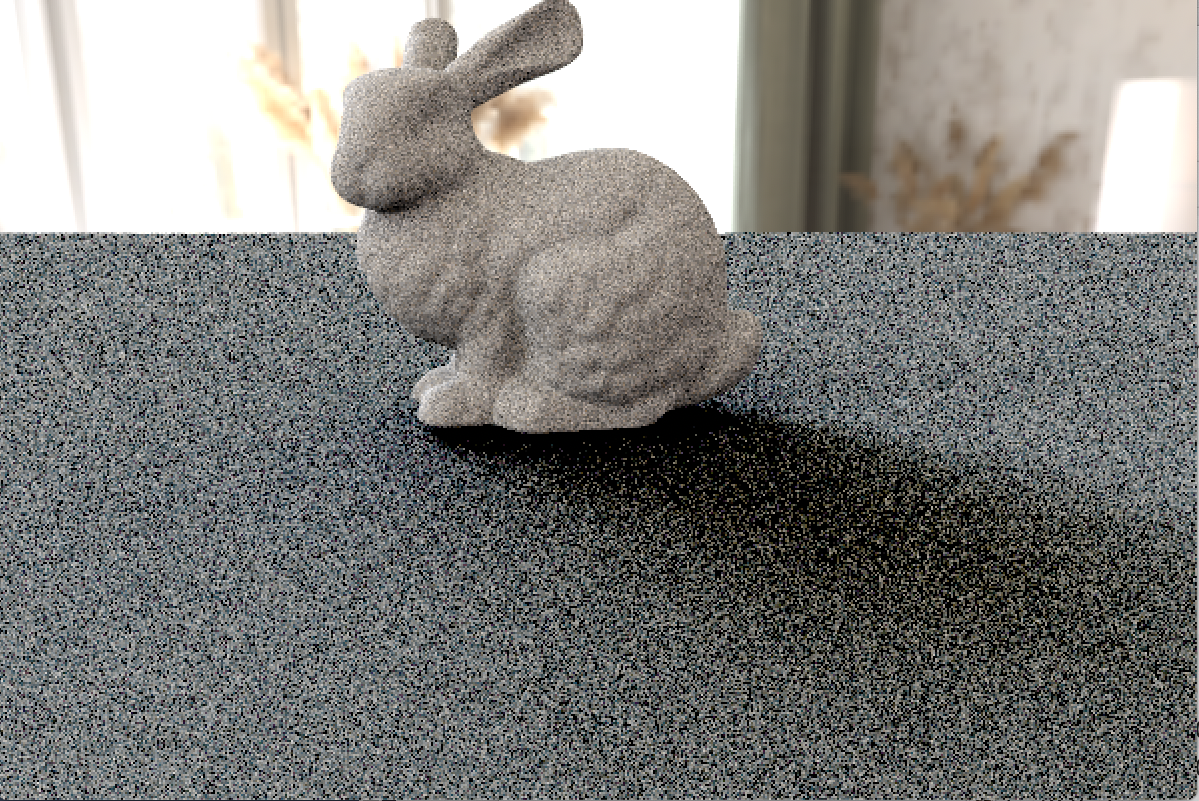
\includegraphics[width=.4\textwidth]{none.png}}
	\subfigure[不添加噪声,进行中值滤波] {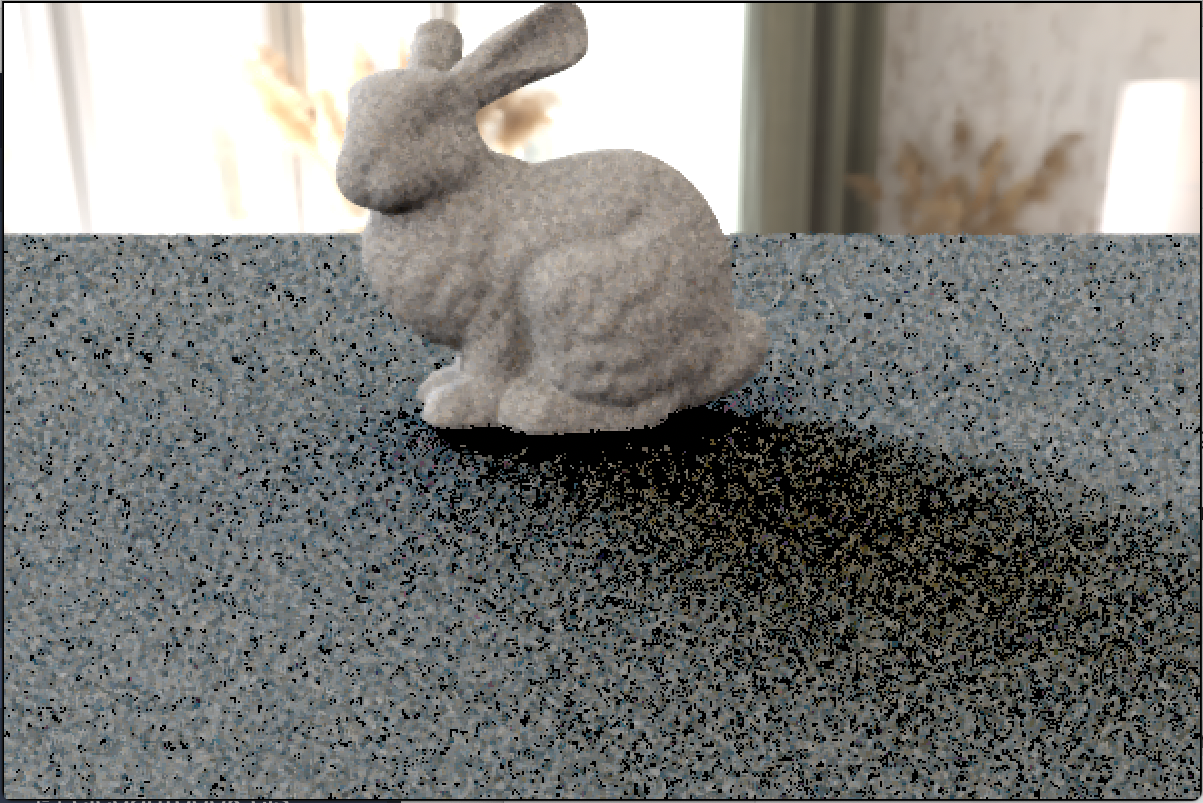
\includegraphics[width=.4\textwidth]{none-median_denoise.png}}
	\caption{不添加噪声,进行中值滤波}
	\label{fig:median_cmp1}
\end{figure}

\begin{figure}[htbp]
	\centering
	\subfigure[渲染得到的原图]{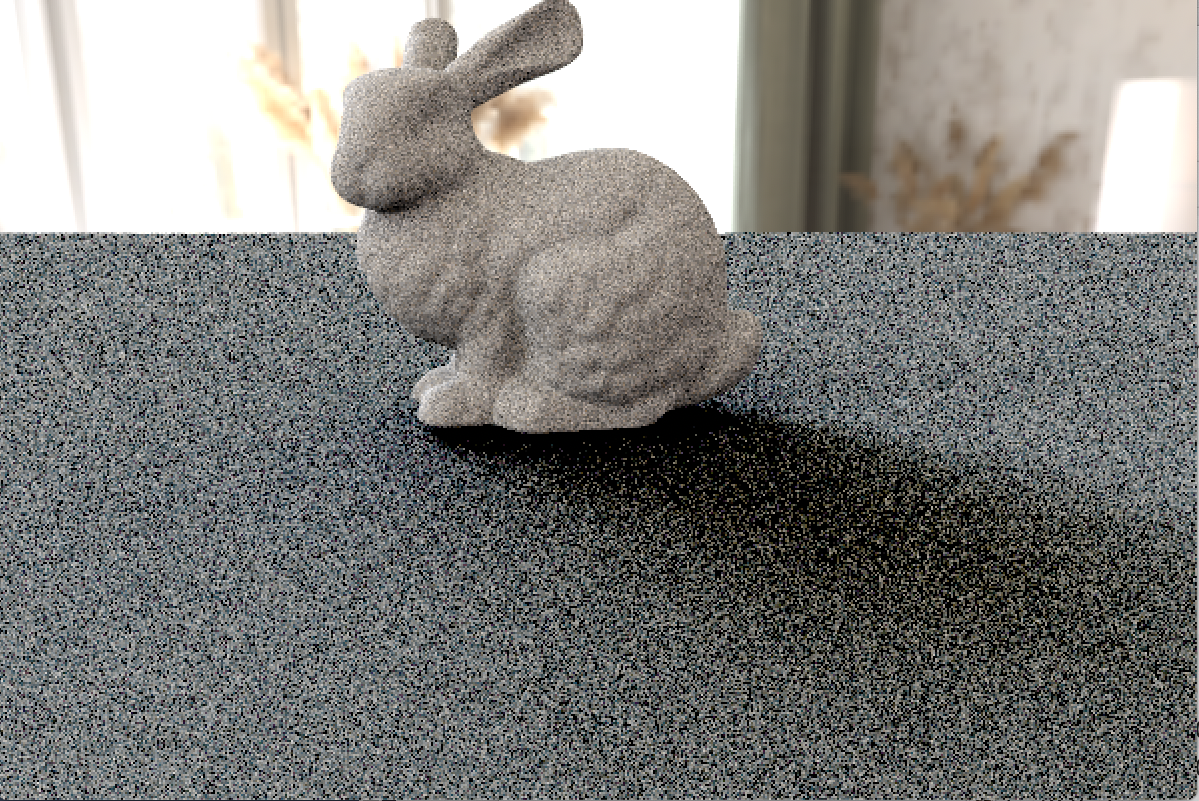
\includegraphics[width=.3\textwidth]{none.png}}
	\subfigure[添加椒盐噪声(n=500)] {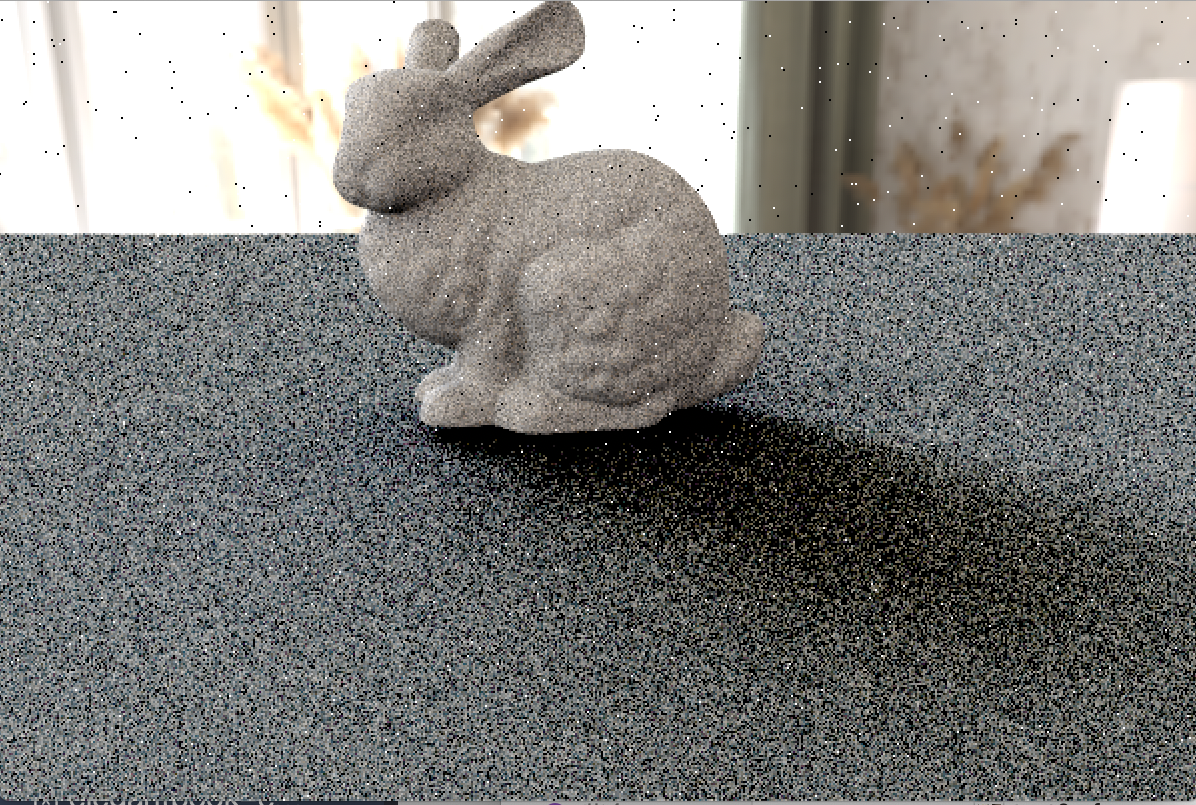
\includegraphics[width=.3\textwidth]{salt_noise(500).png}}
 	\subfigure[进行中值滤波] {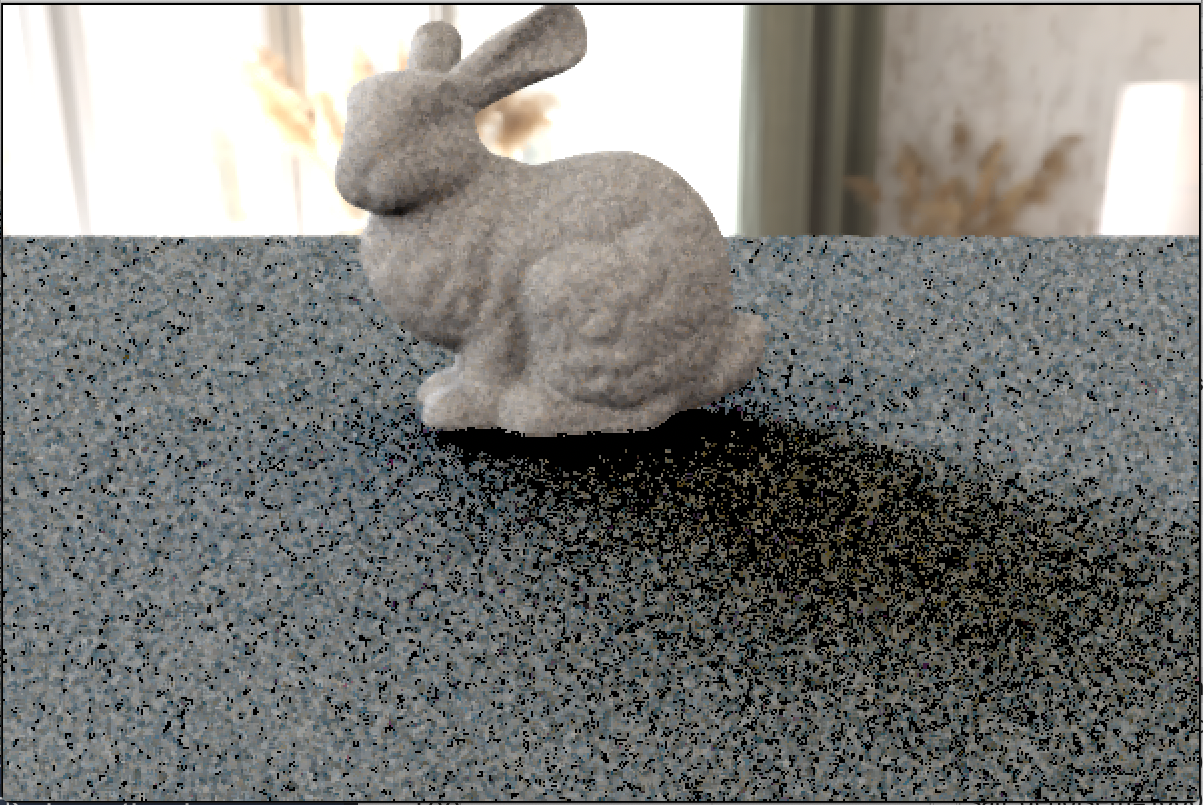
\includegraphics[width=.3\textwidth]{salt_noise(500)-median_denoise.png}}
	\caption{添加椒盐噪声(n=500),进行中值滤波,窗口大小为3}
	\label{fig:median_cmp2.1}
\end{figure}

\begin{figure}[htbp]
	\centering
	\subfigure[渲染得到的原图]{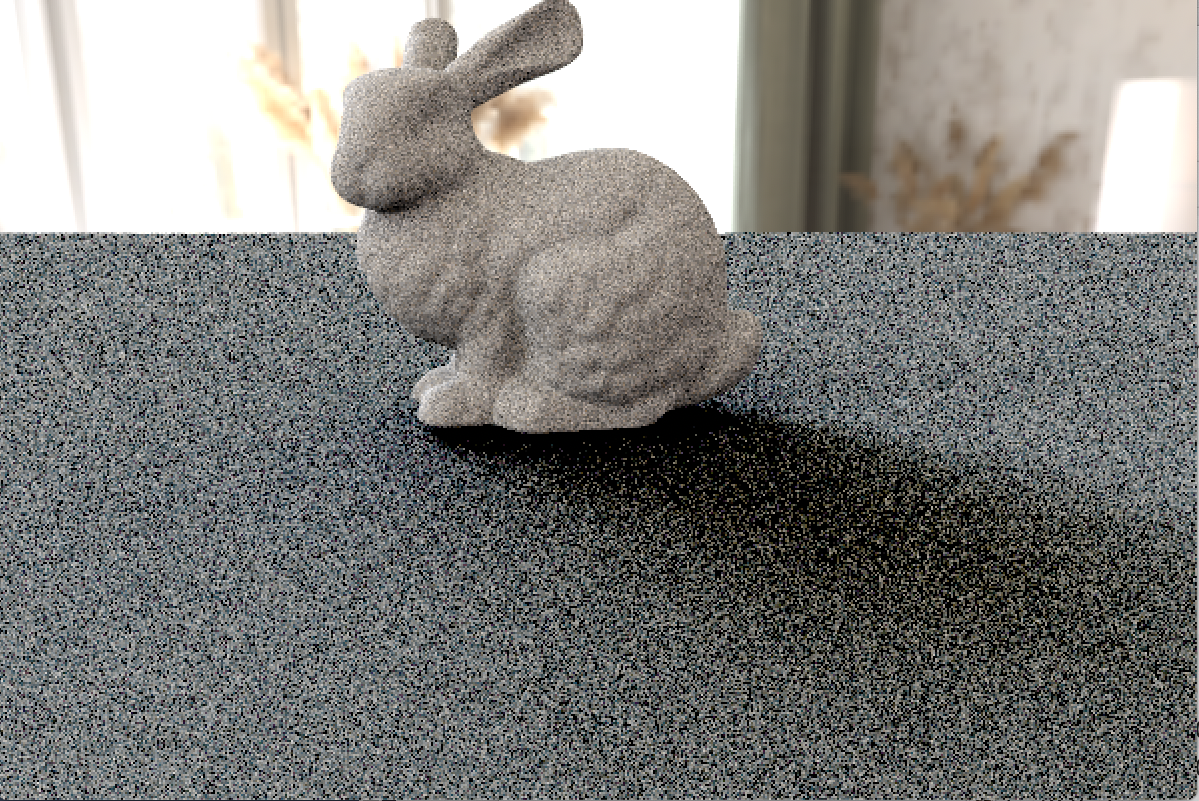
\includegraphics[width=.3\textwidth]{none.png}}
	\subfigure[添加椒盐噪声(n=10000)] {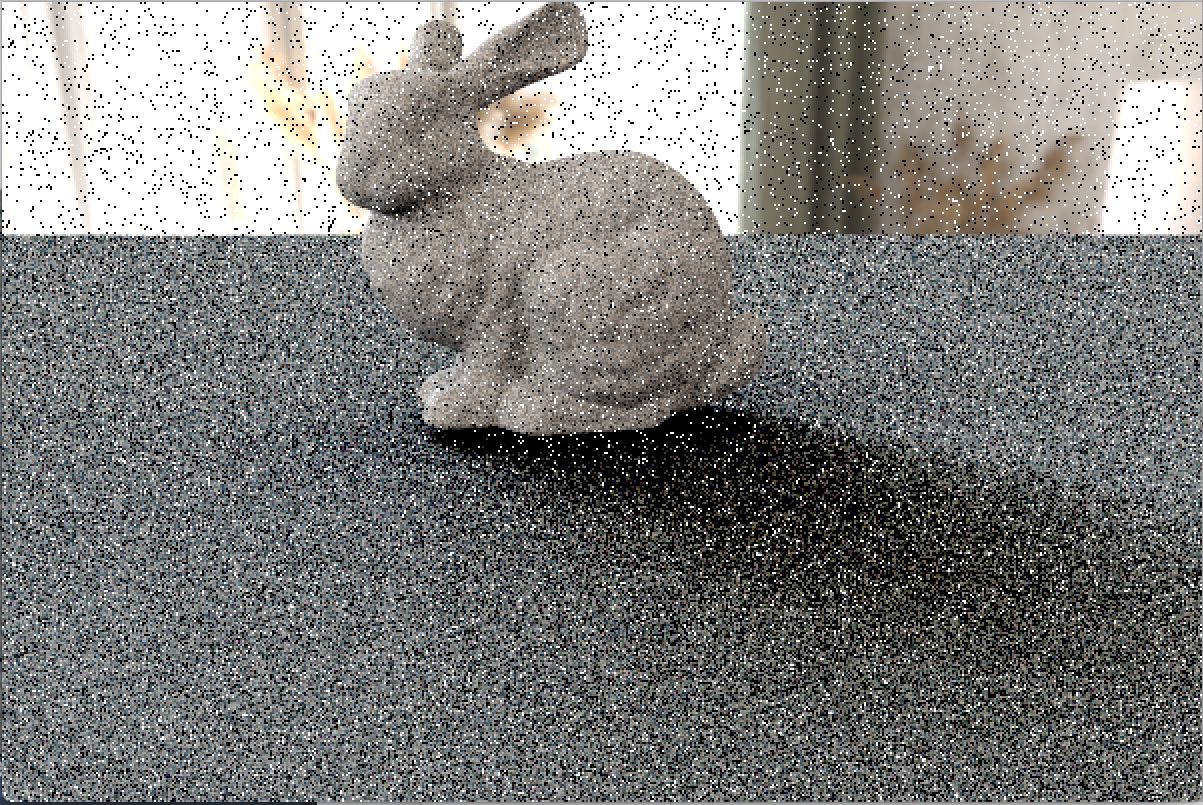
\includegraphics[width=.3\textwidth]{salt_noise(10000).png}}
 	\subfigure[进行中值滤波,窗口大小为3] {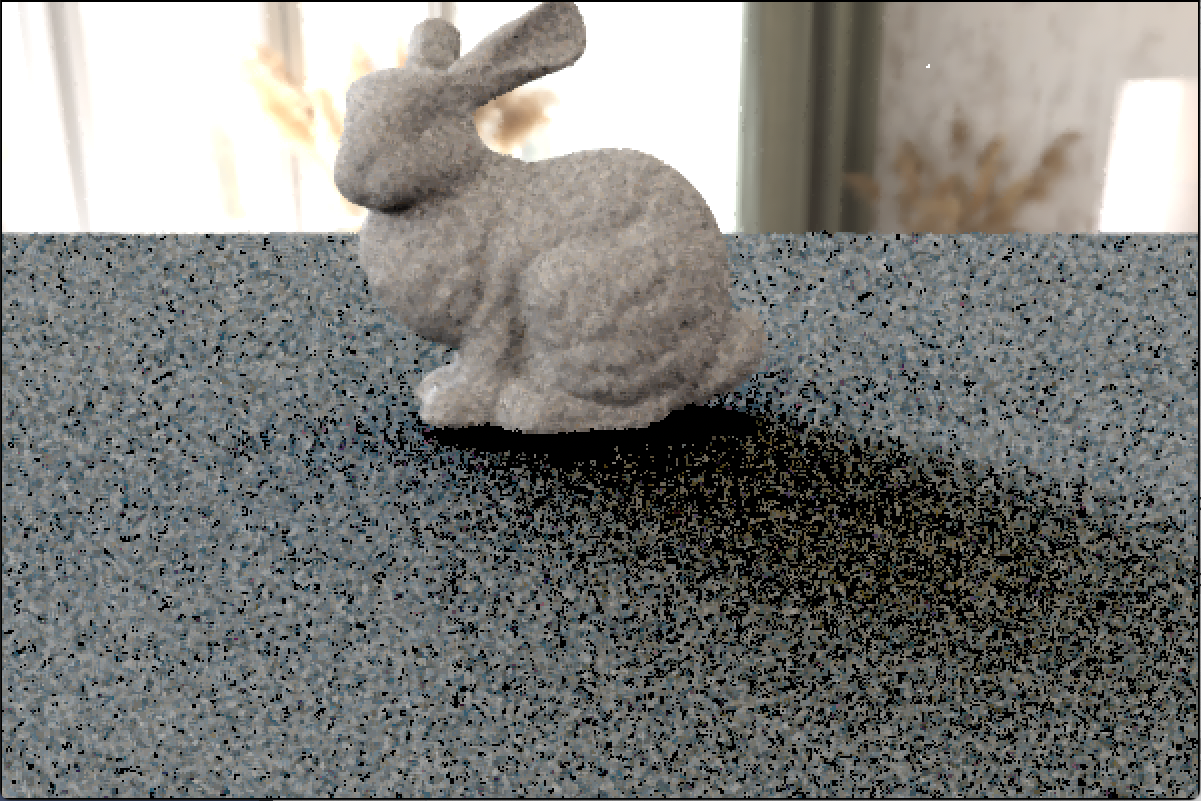
\includegraphics[width=.3\textwidth]{salt_noise(10000)-median_denoise.png}}
	\caption{添加椒盐噪声(n=10000),进行中值滤波,窗口大小为3}
	\label{fig:median_cmp2.2}
\end{figure}

\begin{figure}[htbp]
	\centering
	\subfigure[渲染得到的原图]{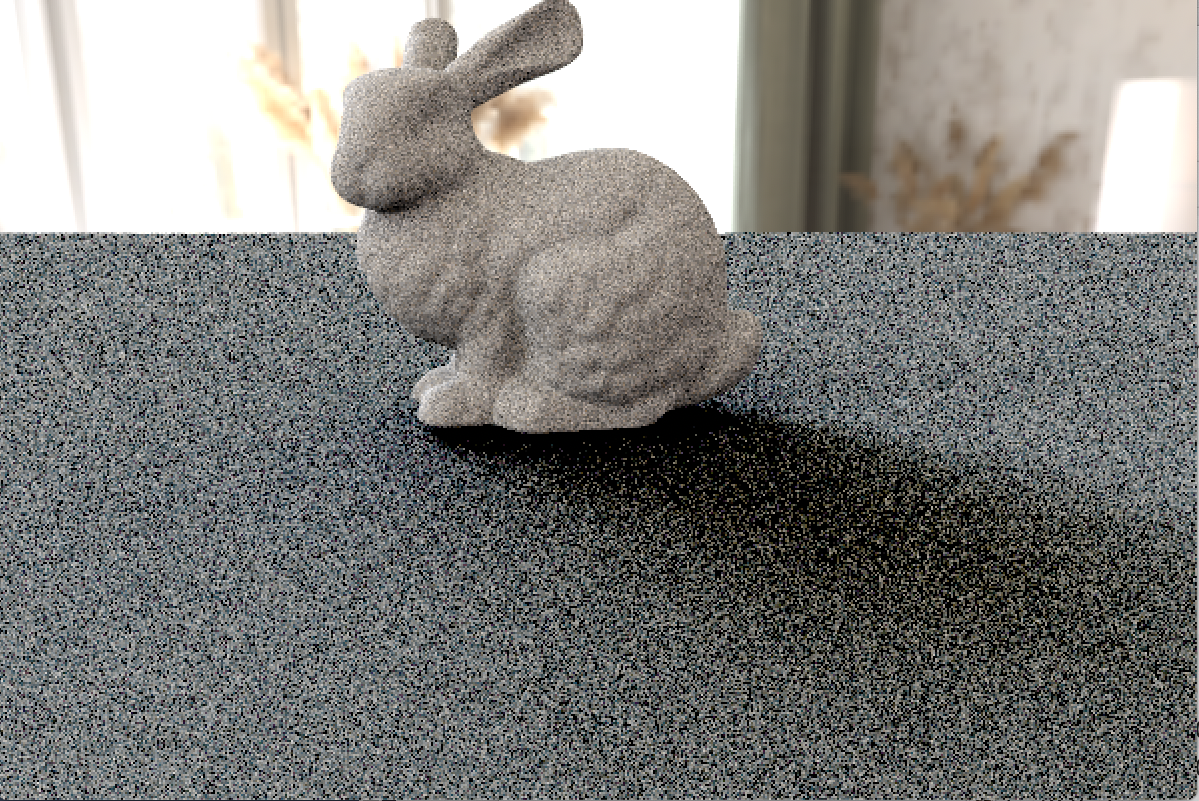
\includegraphics[width=.3\textwidth]{none.png}}
	\subfigure[添加椒盐噪声(n=10000)] {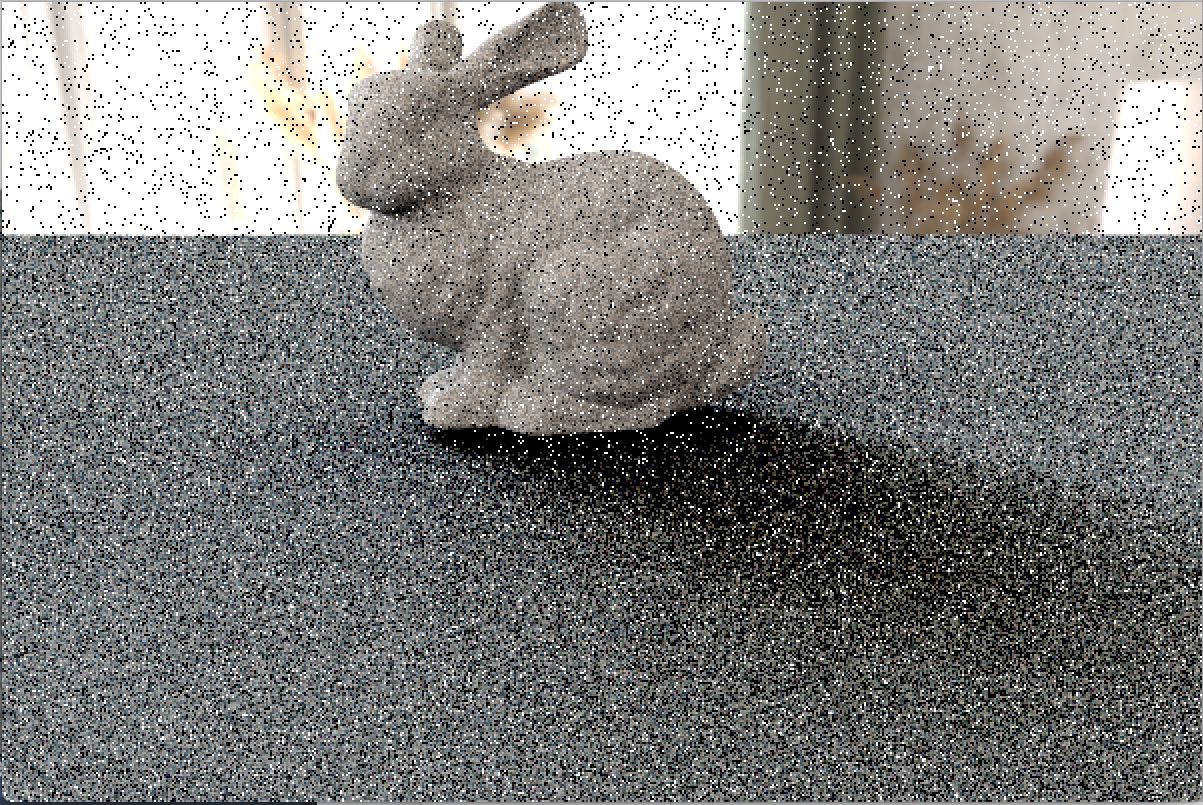
\includegraphics[width=.3\textwidth]{salt_noise(10000).png}}
 	\subfigure[进行中值滤波,窗口大小为21] {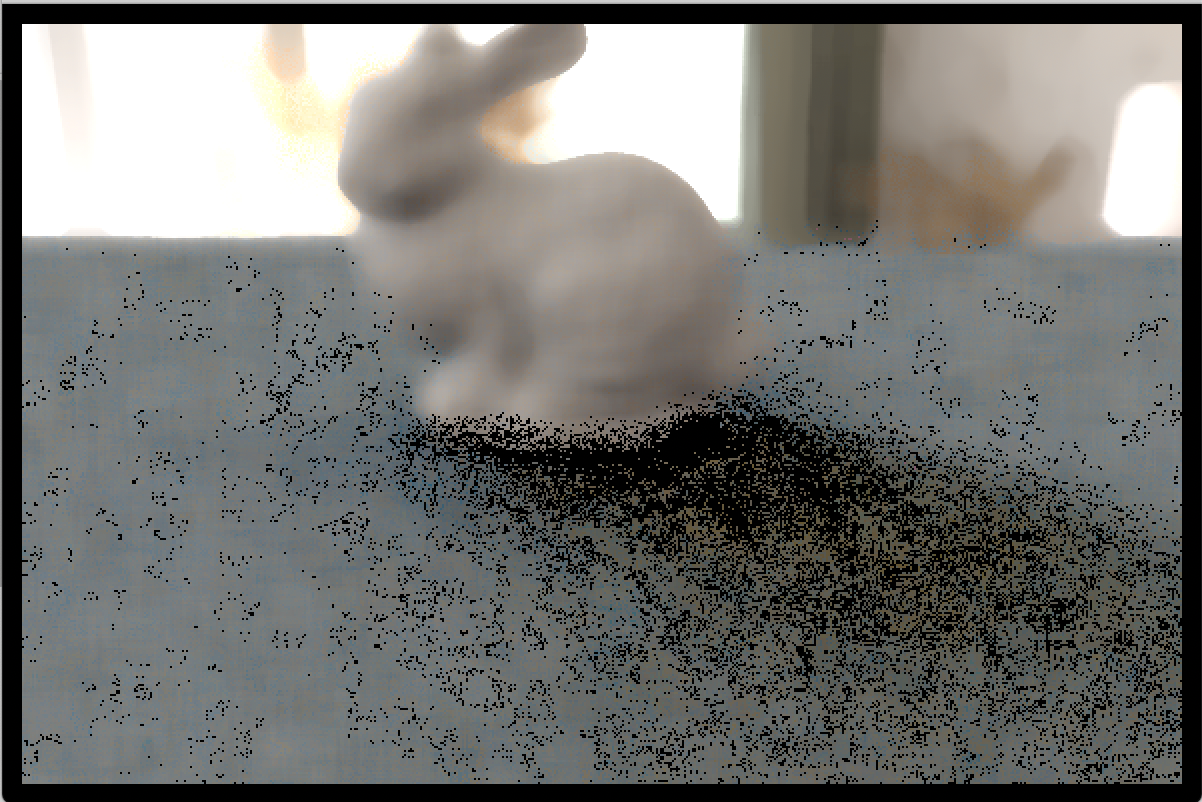
\includegraphics[width=.3\textwidth]{salt_noise(10000)-median_denoise21.png}}
	\caption{添加椒盐噪声(n=10000),进行中值滤波,窗口大小为21}
	\label{fig:median_cmp4}
\end{figure}


\begin{figure}[htbp]
	\centering
	\subfigure[渲染得到的原图]{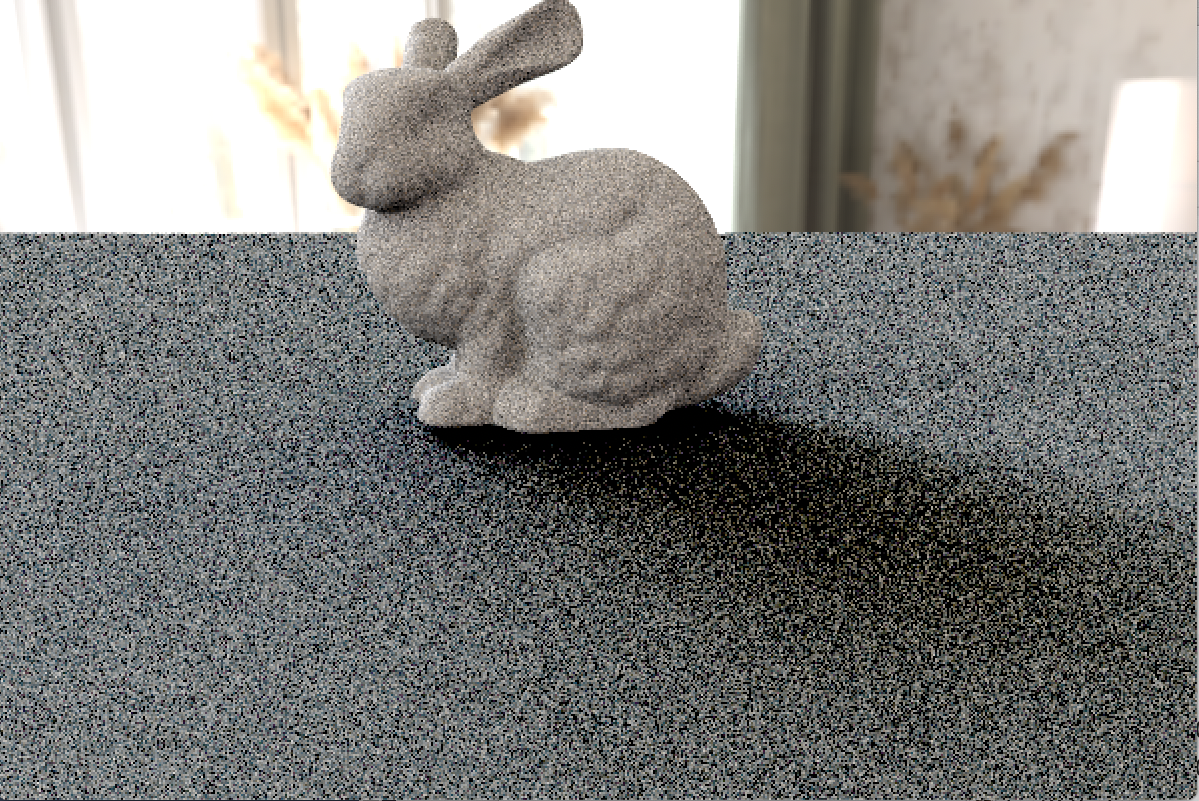
\includegraphics[width=.3\textwidth]{none.png}}
	\subfigure[添加高斯噪声($\sigma=0.1$)] {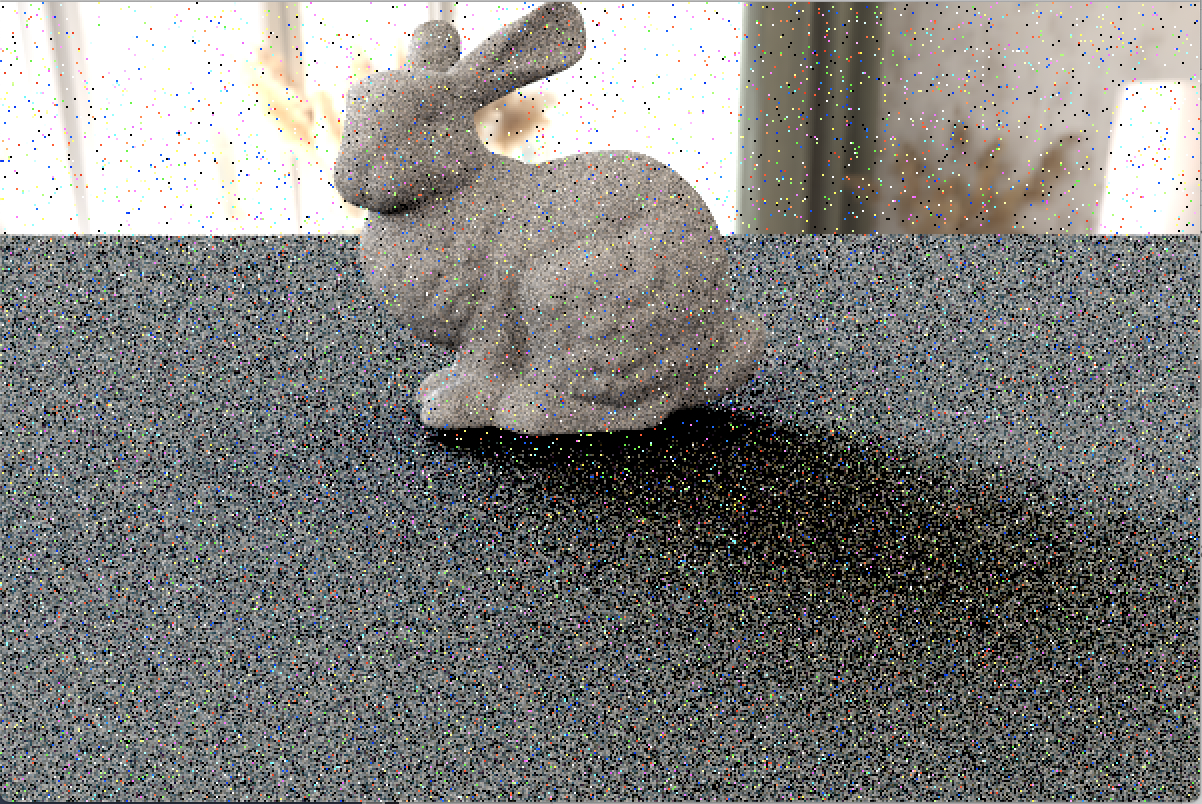
\includegraphics[width=.3\textwidth]{g_noise(20,0.1).png}}
    \subfigure[进行中值滤波,窗口大小为3] {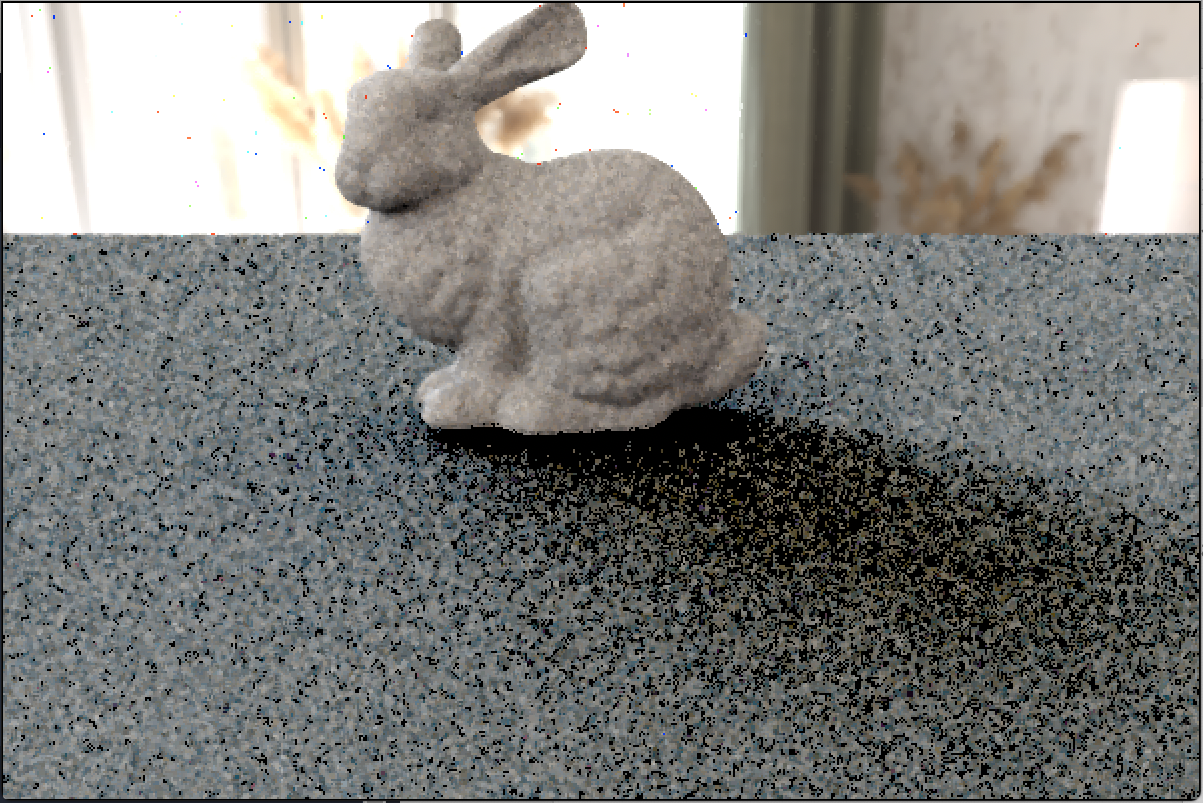
\includegraphics[width=.3\textwidth]{g_noise(20,0.1)-median_denoise.png}}
	\caption{添加高斯噪声($\sigma=0.1$),进行中值滤波,窗口大小为3}
	\label{fig:median_cmp3.1}
\end{figure}

\begin{figure}[htbp]
	\centering
	\subfigure[渲染得到的原图]{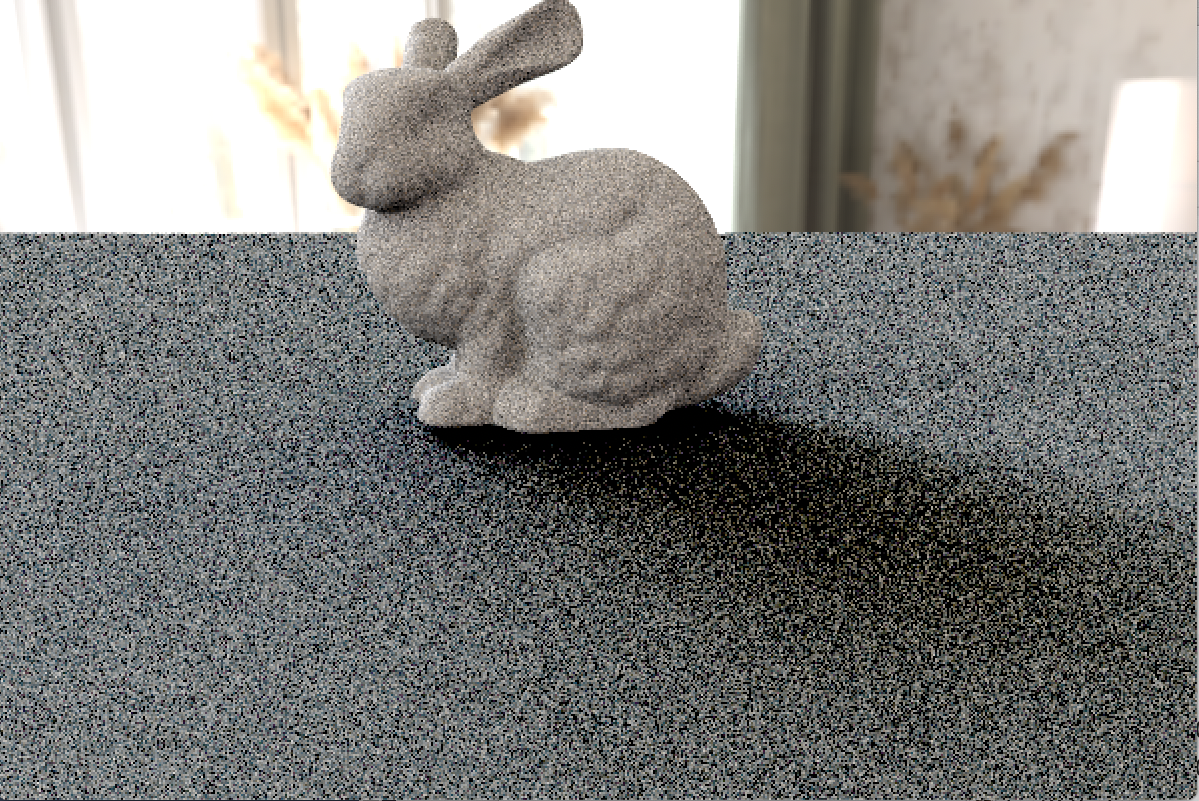
\includegraphics[width=.3\textwidth]{none.png}}
	\subfigure[添加高斯噪声($\sigma=1$)] {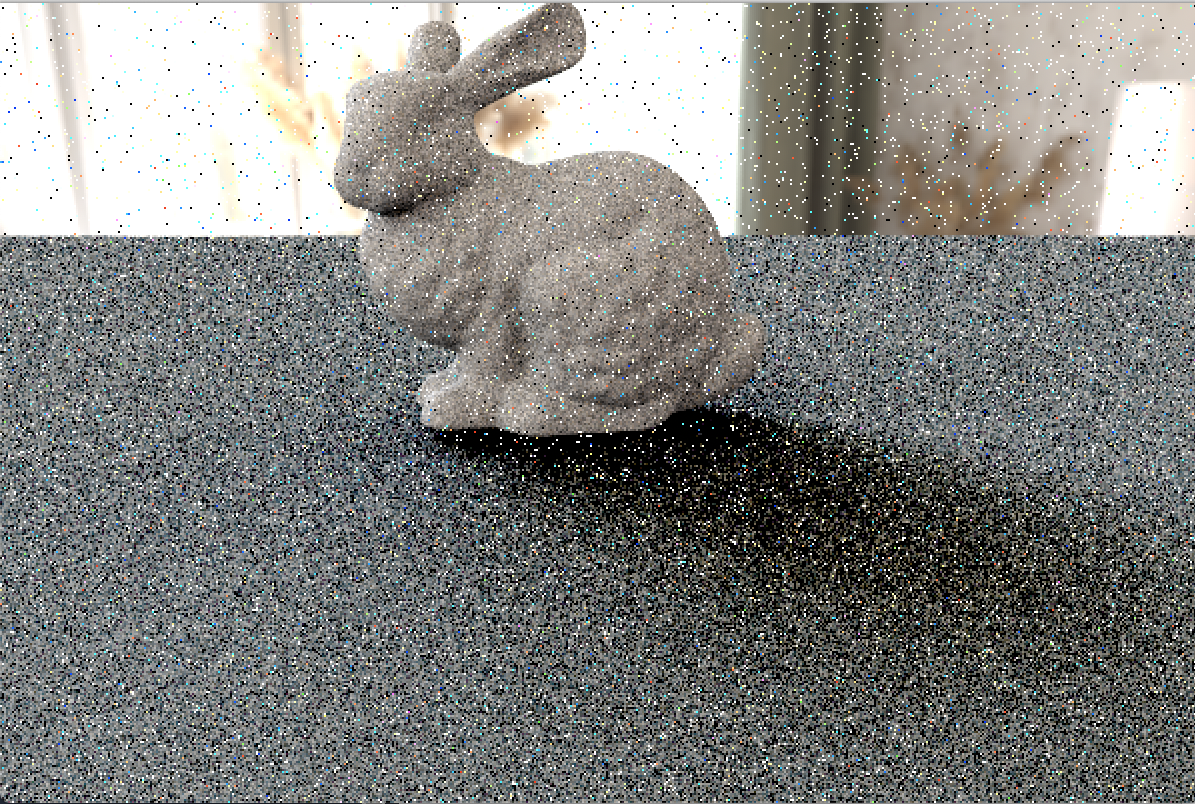
\includegraphics[width=.3\textwidth]{g_noise(20,1).png}}
    \subfigure[进行中值滤波,窗口大小为3] {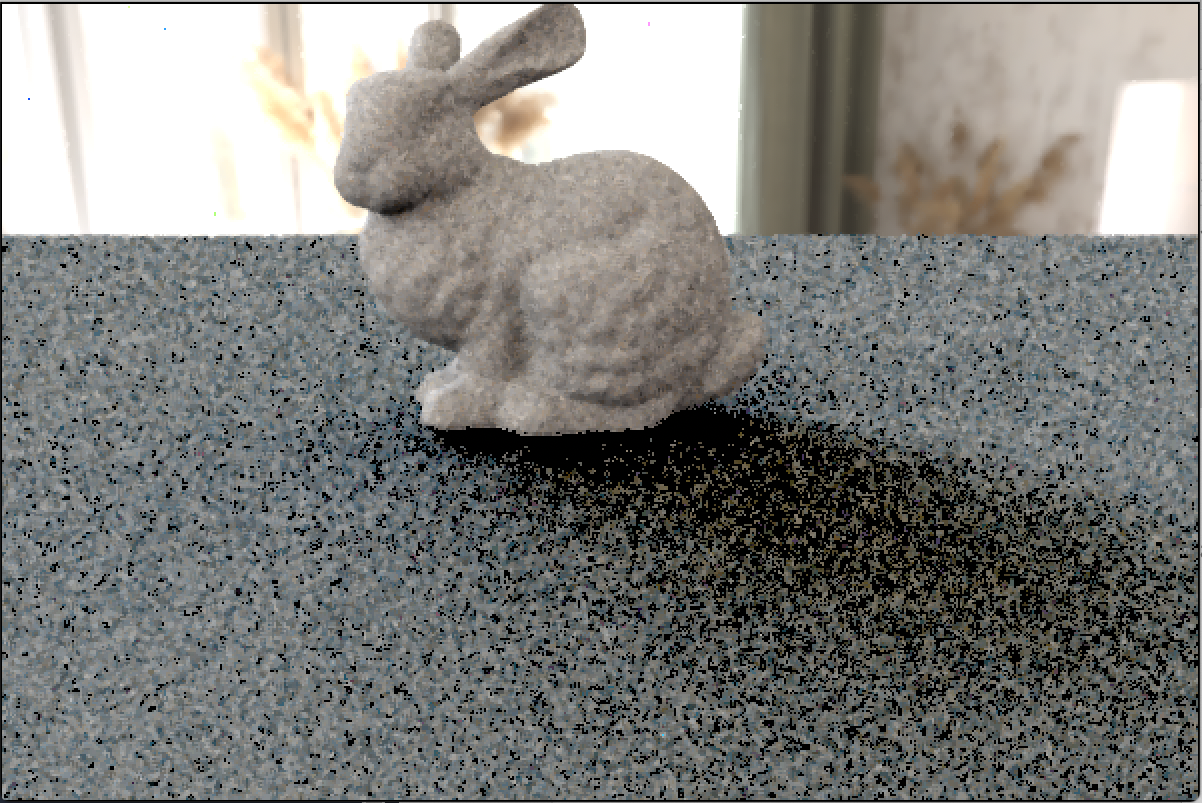
\includegraphics[width=.3\textwidth]{g_noise(20,1)-median_denoise.png}}
	\caption{添加高斯噪声($\sigma=1$),进行中值滤波,窗口大小为3}
	\label{fig:median_cmp3.2}
\end{figure}

\begin{figure}[htbp]
	\centering
	\subfigure[渲染得到的原图]{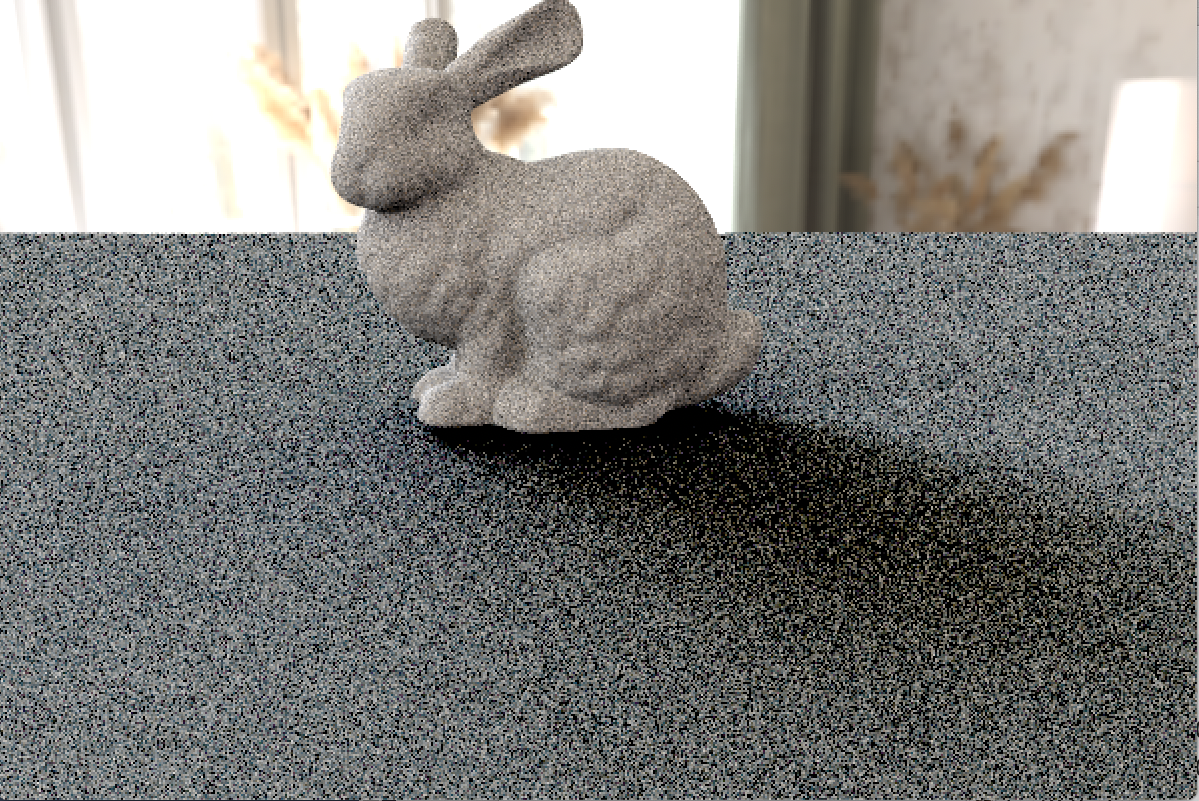
\includegraphics[width=.3\textwidth]{none.png}}
	\subfigure[添加高斯噪声($\sigma=100$)] {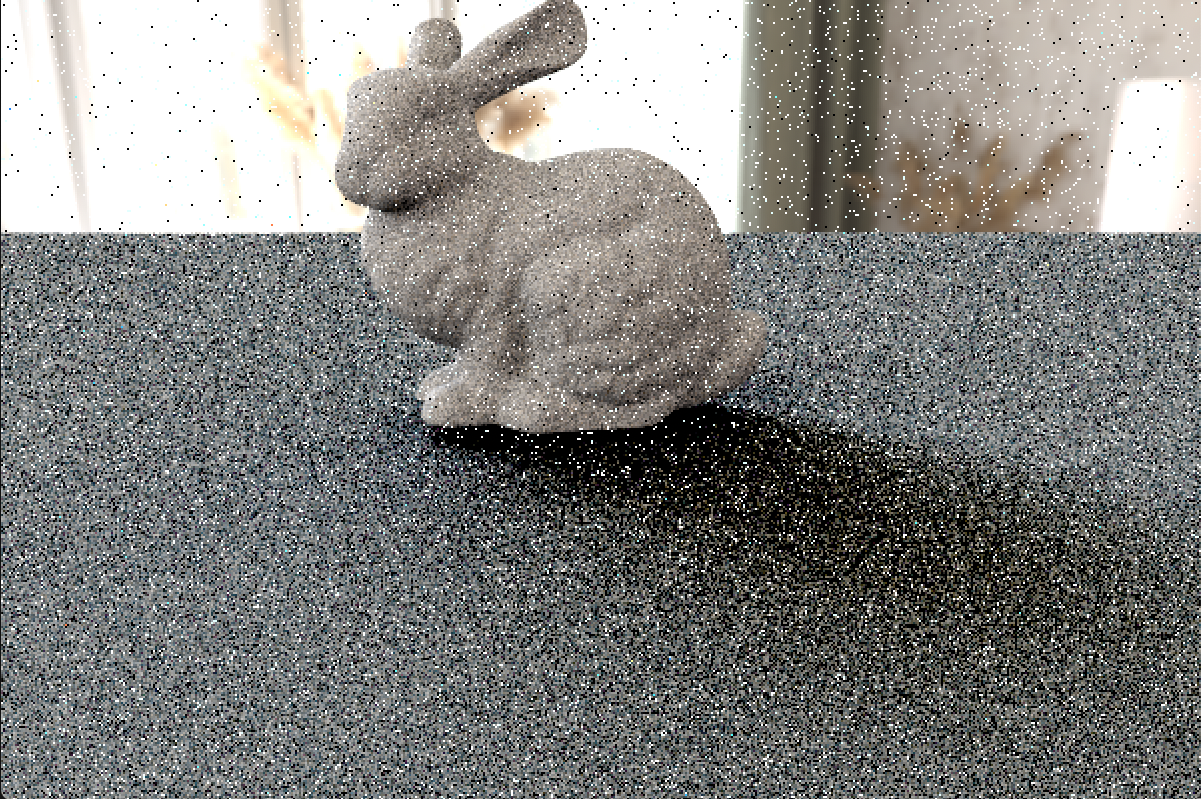
\includegraphics[width=.3\textwidth]{g_noise(20,100).png}}
    \subfigure[进行中值滤波,窗口大小为3] {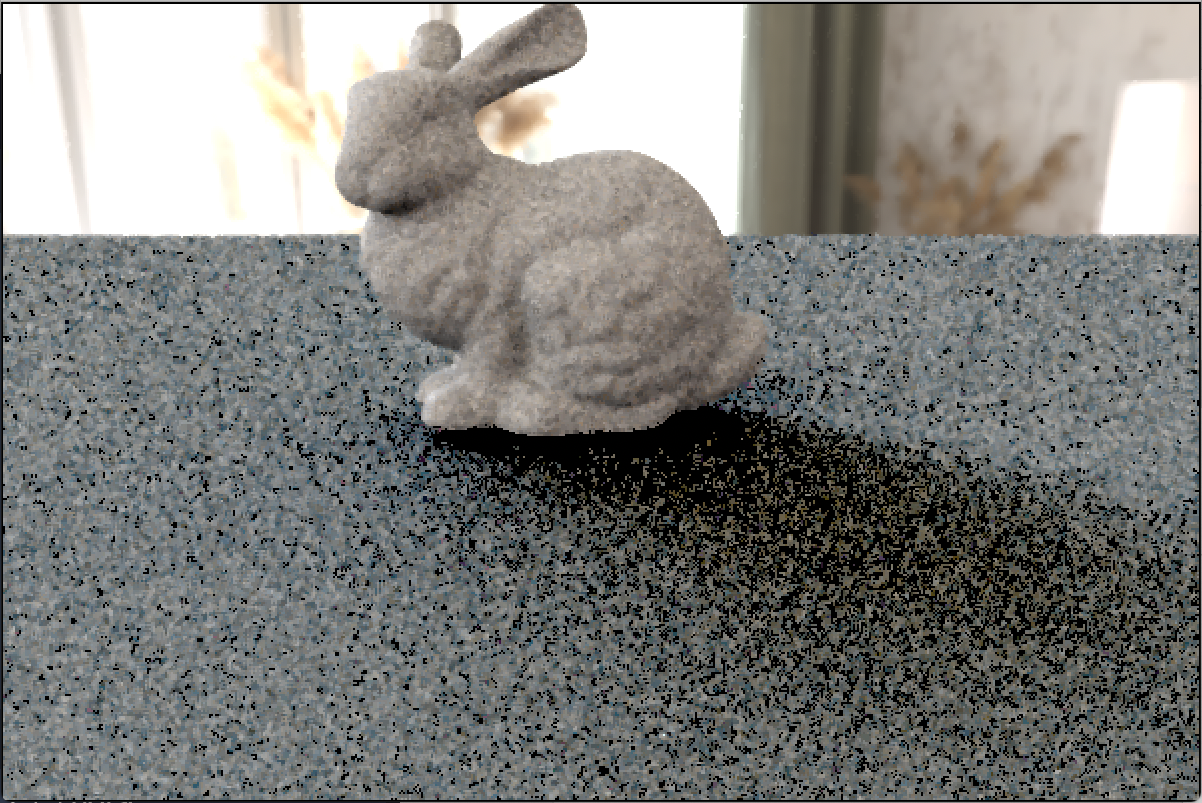
\includegraphics[width=.3\textwidth]{g_noise(20,100)-median_denoise.png}}
	\caption{添加高斯噪声($\sigma=100$),进行中值滤波}
	\label{fig:median_cmp3.3}
\end{figure}


\vspace{50pt}
\quad \textcolor{second}{\textbf{分析:}}
\begin{itemize}
\item 滤波后的图片四周出现黑边,是由于在滤波时,在图片的扩展边界填充0。中值滤波的窗口越大,则黑边越宽。

\item 椒盐噪声点越少,中值滤波的平滑效果越好。

\item 高斯噪声中$\sigma$越大,中值滤波的平滑效果越好。

\item 中值滤波对椒盐噪声表现较好,对高斯噪声表现较差。

\end{itemize}


\subsection{均值滤波}

在分析均值滤波的效果时,一共做了四组对比实验:
\vspace{5pt}
\begin{enumerate}[itemsep=1.5ex]

\item 对照组:使用均值滤波过滤未添加噪声的图片。如图~\ref{fig:mean_cmp1}所示。

\item 同样大小的窗口对不同程度的椒盐噪声的去噪效果:使用窗口大小为3的均值滤波过滤添加椒盐噪声的图片,n的取值包含500、10000。如图~\ref{fig:mean_cmp2.1}和~\ref{fig:mean_cmp2.2}所示。

\item 同样大小的窗口对不同程度的高斯噪声的去噪效果:使用窗口大小为3的均值滤波过滤添加高斯噪声的图片,$\sigma$取值包含0.1、1、100,数据处理范围为20\%。如图~\ref{fig:mean_cmp3.1}、~\ref{fig:mean_cmp3.2}和~\ref{fig:mean_cmp3.3}所示。

\item 不同大小的窗口对同样程度的高斯噪声的去噪效果:使用窗口大小为3、21的均值滤波过滤添加椒盐噪声的图片。如图~\ref{fig:mean_cmp3.1}和~\ref{fig:mean_cmp4}所示。

\end{enumerate}

\begin{figure}[htbp]
	\centering
	\subfigure[渲染得到的原图]{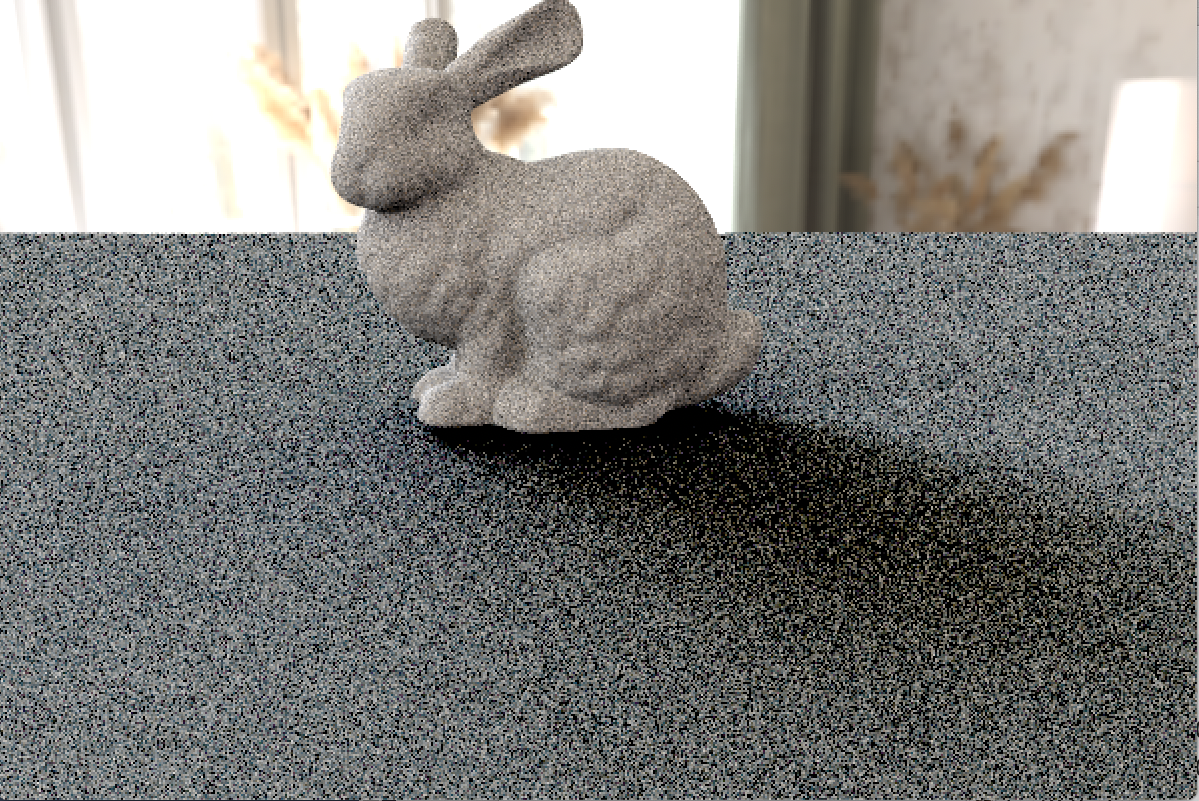
\includegraphics[width=.4\textwidth]{none.png}}
	\subfigure[进行均值滤波] {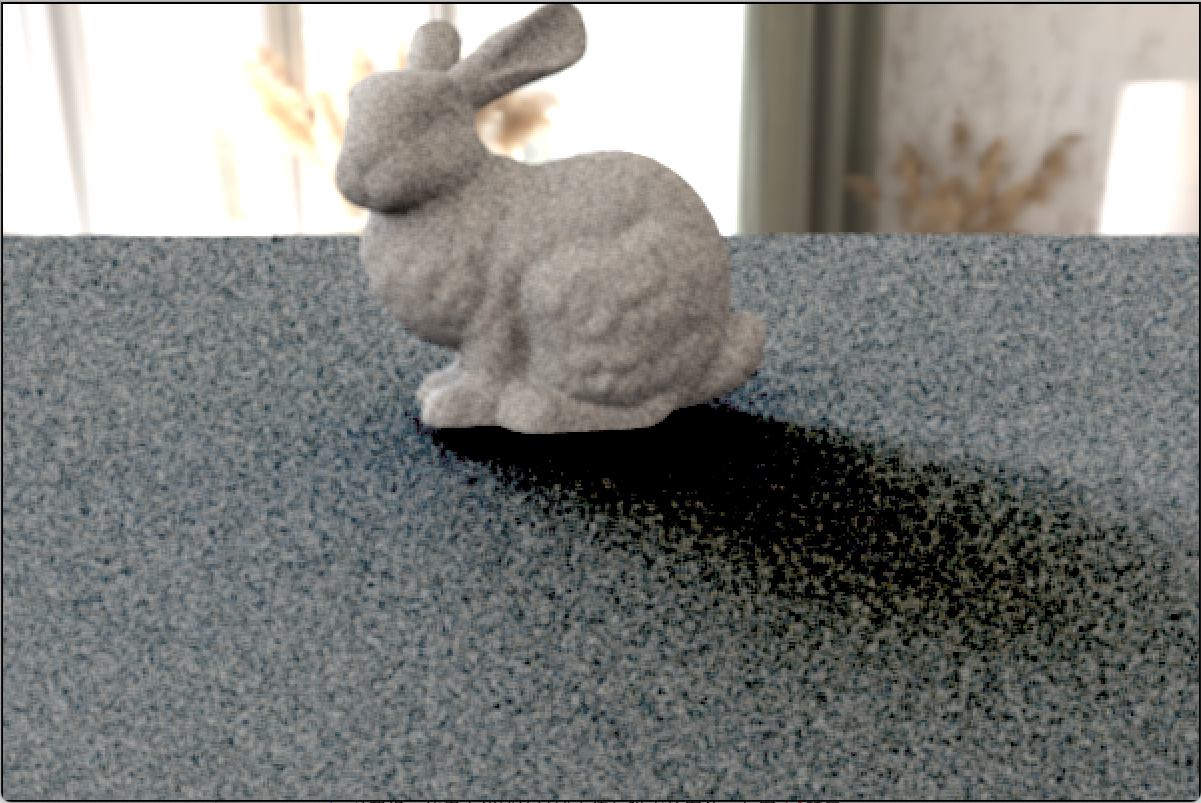
\includegraphics[width=.4\textwidth]{none-mean_denoise.png}}
	\caption{不添加噪声,进行均值滤波}
	\label{fig:mean_cmp1}
\end{figure}

\begin{figure}[htbp]
	\centering
	\subfigure[渲染得到的原图]{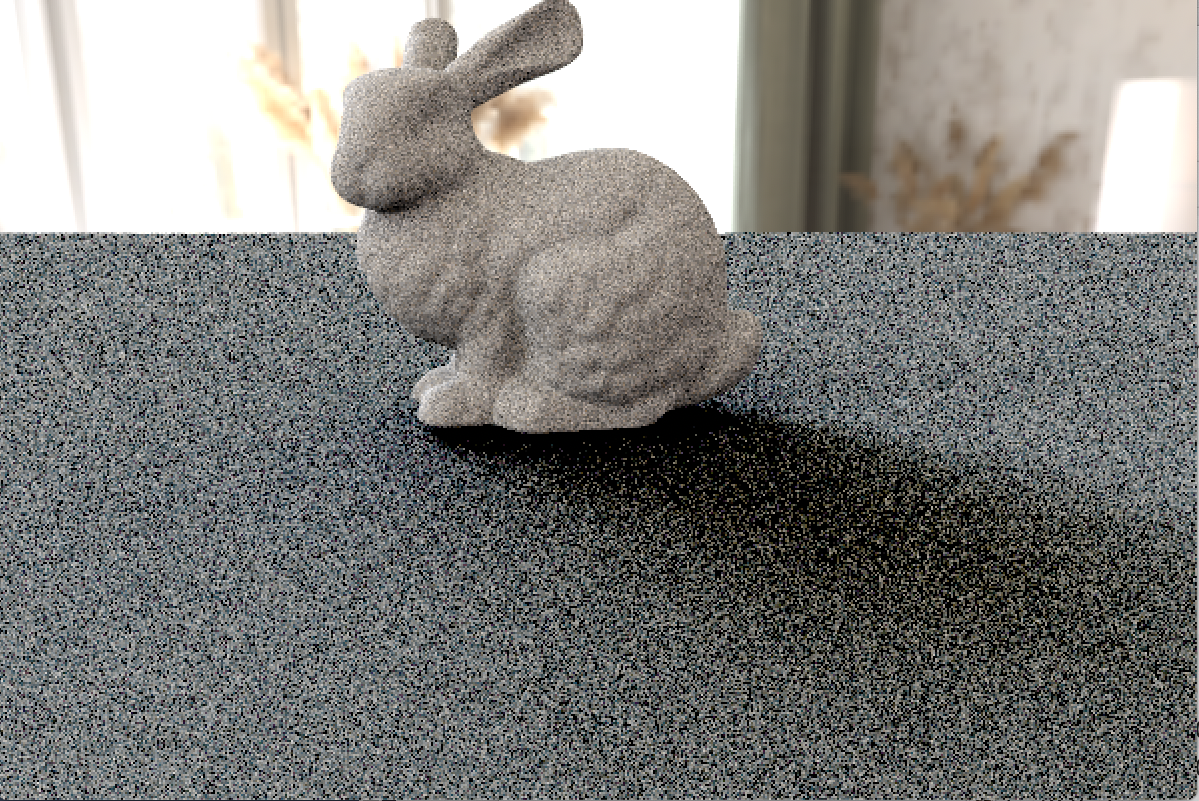
\includegraphics[width=.3\textwidth]{none.png}}
	\subfigure[添加椒盐噪声(n=500)] {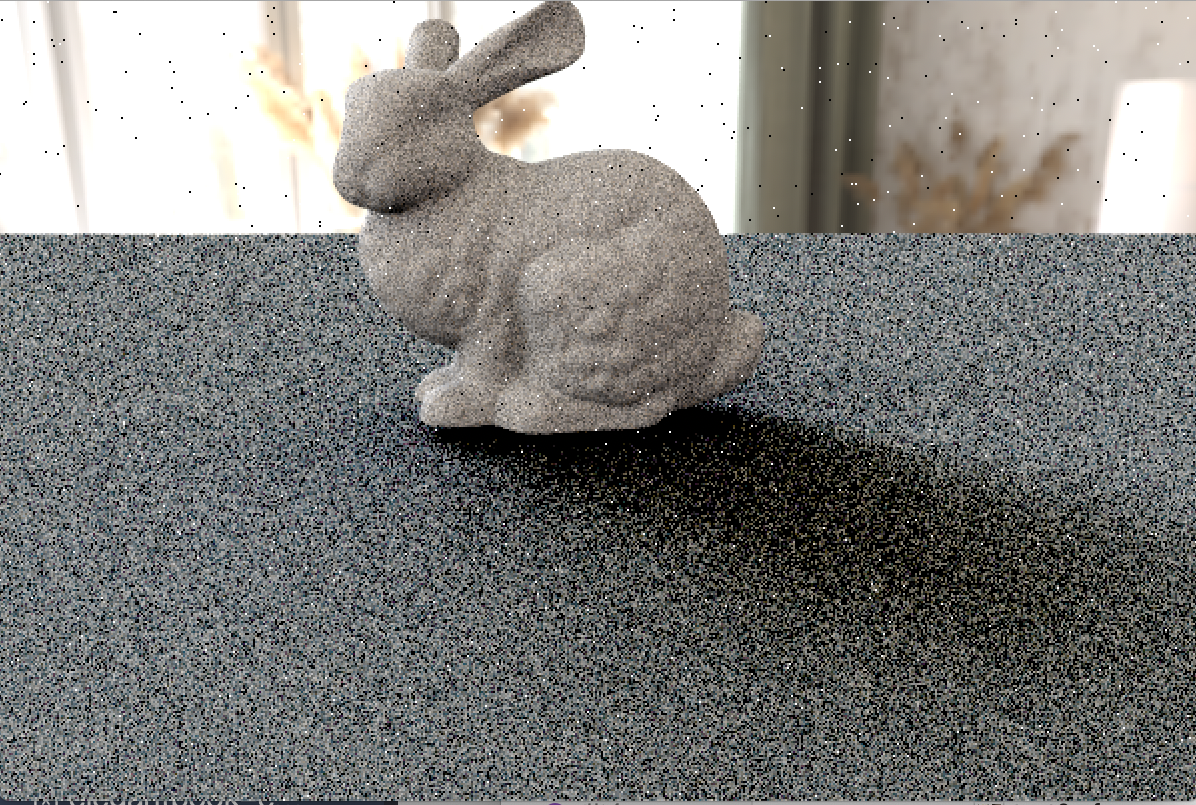
\includegraphics[width=.3\textwidth]{salt_noise(500).png}}
 	\subfigure[进行均值滤波,窗口大小为3] {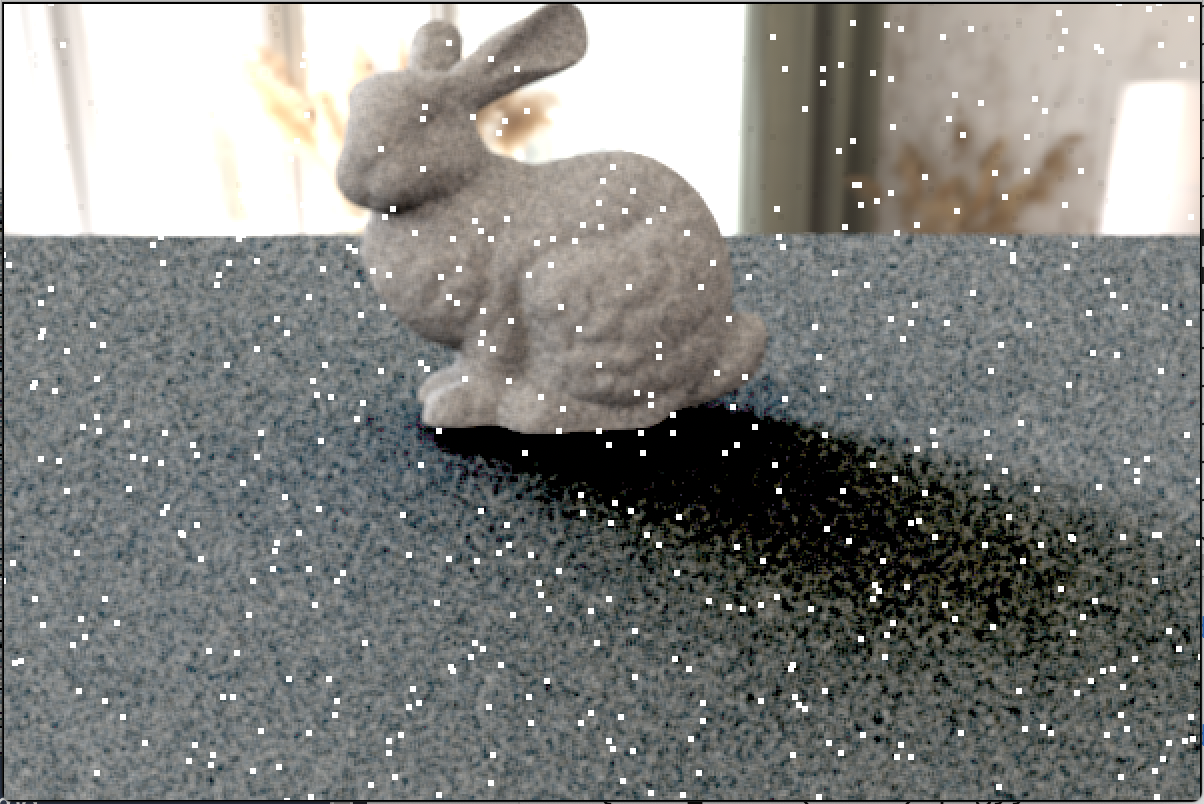
\includegraphics[width=.3\textwidth]{salt_noise(500)-mean_denoise.png}}
	\caption{添加椒盐噪声(n=500),进行均值滤波,窗口大小为3}
	\label{fig:mean_cmp2.1}
\end{figure}

\begin{figure}[htbp]
	\centering
	\subfigure[渲染得到的原图]{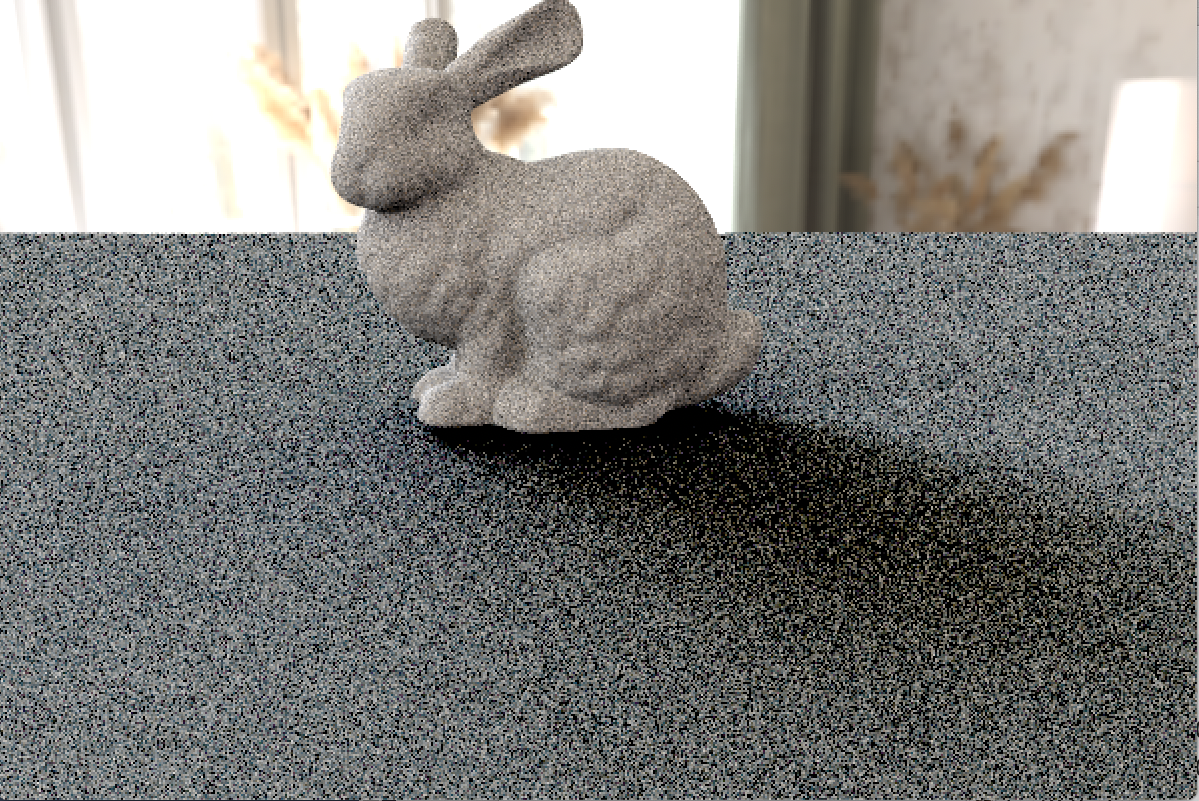
\includegraphics[width=.3\textwidth]{none.png}}
	\subfigure[添加椒盐噪声(n=10000)] {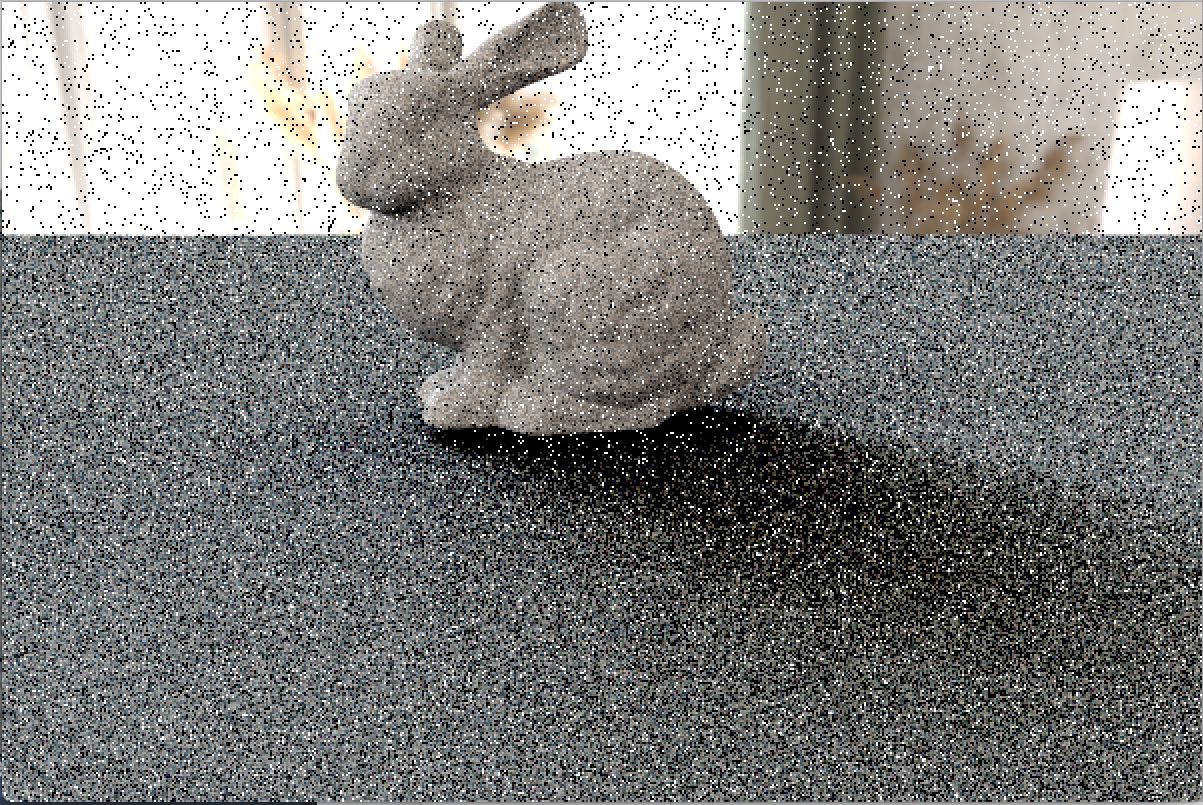
\includegraphics[width=.3\textwidth]{salt_noise(10000).png}}
 	\subfigure[进行均值滤波,窗口大小为3] {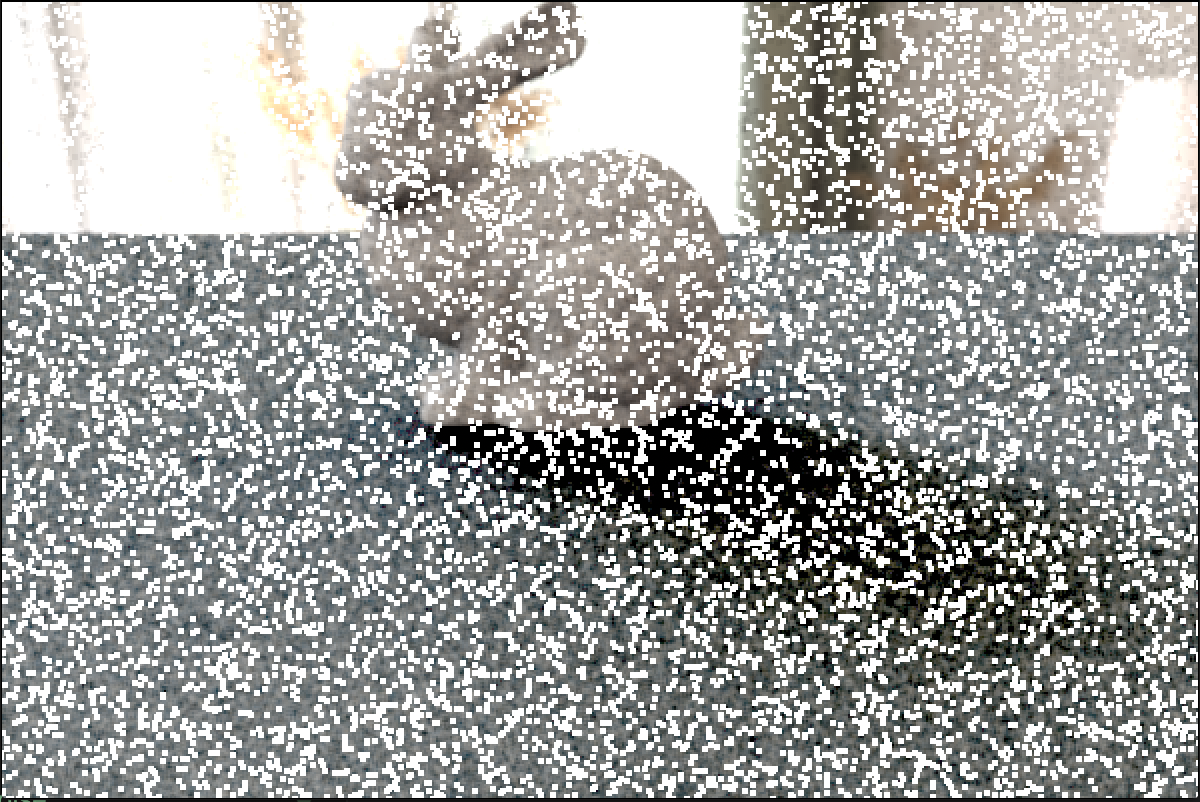
\includegraphics[width=.3\textwidth]{salt_noise(10000)-mean_denoise.png}}
	\caption{添加椒盐噪声(n=10000),进行均值滤波,窗口大小为3}
	\label{fig:mean_cmp2.2}
\end{figure}

\begin{figure}[htbp]
	\centering
	\subfigure[渲染得到的原图]{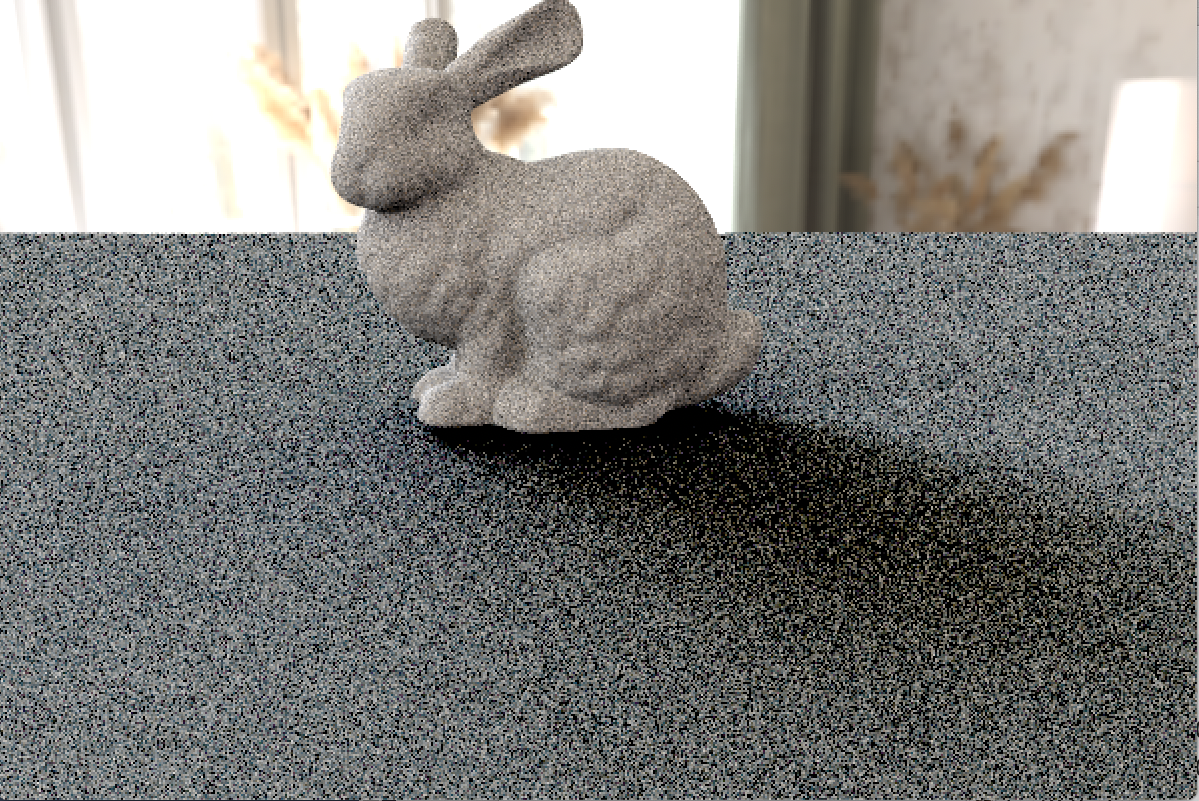
\includegraphics[width=.3\textwidth]{none.png}}
	\subfigure[添加高斯噪声($\sigma=0.1$)] {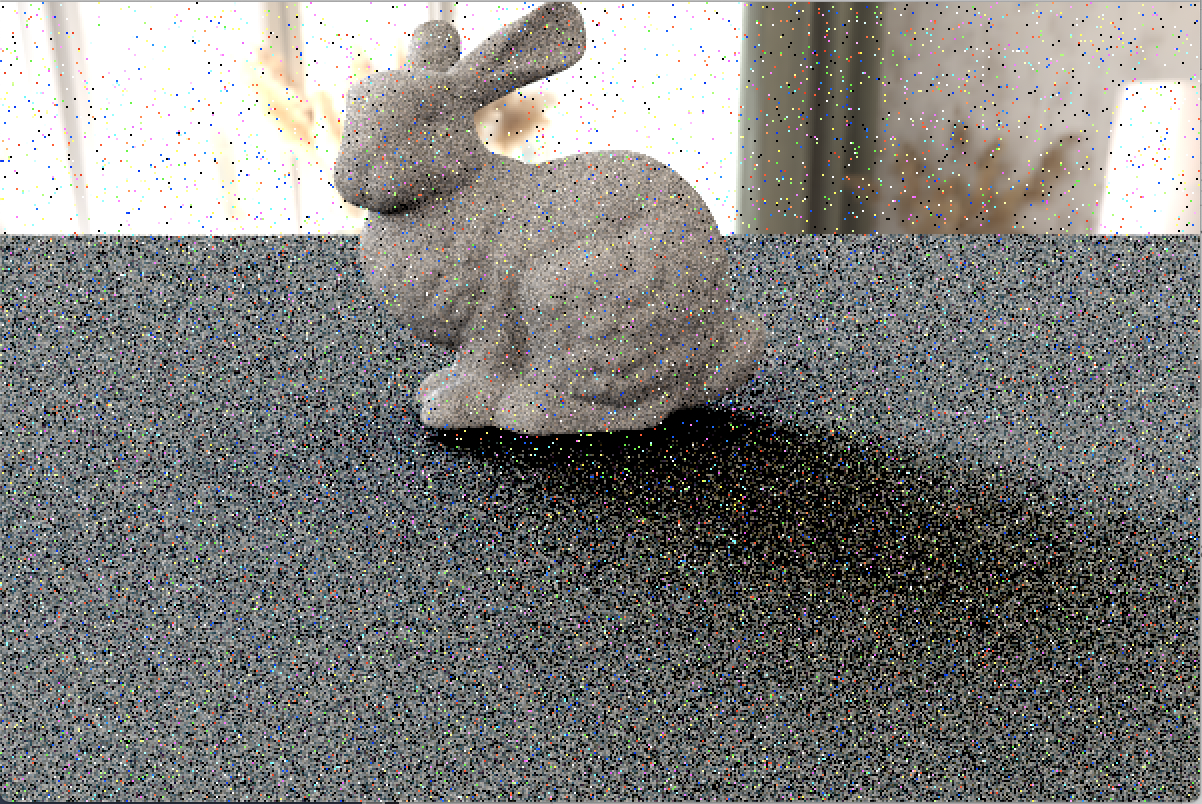
\includegraphics[width=.3\textwidth]{g_noise(20,0.1).png}}
    \subfigure[进行均值滤波,窗口大小为3] {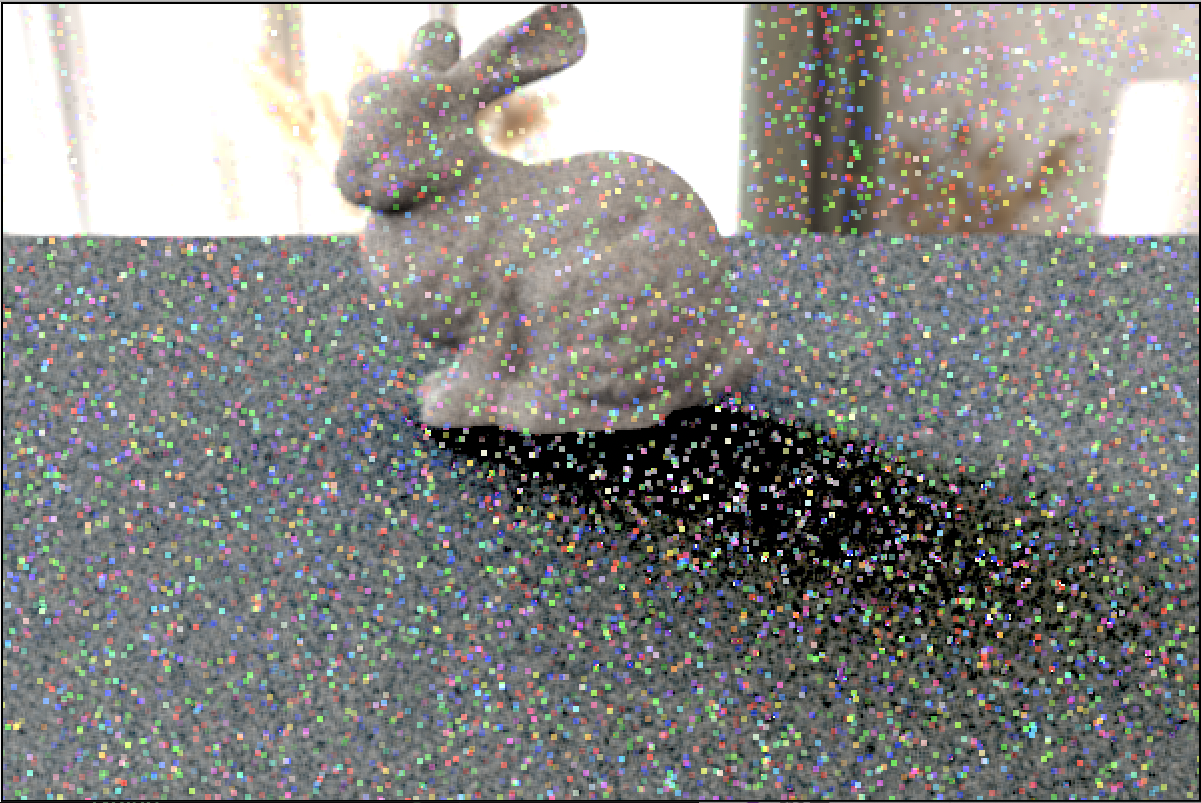
\includegraphics[width=.3\textwidth]{g_noise(20,0.1)-mean_denoise.png}}
	\caption{添加高斯噪声($\sigma=0.1$),进行均值滤波,窗口大小为3}
	\label{fig:mean_cmp3.1}
\end{figure}

\begin{figure}[htbp]
	\centering
	\subfigure[渲染得到的原图]{\includegraphics[width=.3\textwidth]{none.png}}
	\subfigure[添加高斯噪声($\sigma=1$)] {\includegraphics[width=.3\textwidth]{g_noise(20,1).png}}
    \subfigure[进行均值滤波,窗口大小为3] {\includegraphics[width=.3\textwidth]{g_noise(20,1)-mean_denoise.png}}
	\caption{添加高斯噪声($\sigma=1$),进行均值滤波,窗口大小为3}
	\label{fig:mean_cmp3.2}
\end{figure}

\begin{figure}[htbp]
	\centering
	\subfigure[渲染得到的原图]{\includegraphics[width=.3\textwidth]{none.png}}
	\subfigure[添加高斯噪声($\sigma=100$)] {\includegraphics[width=.3\textwidth]{g_noise(20,100).png}}
    \subfigure[进行均值滤波,窗口大小为3] {\includegraphics[width=.3\textwidth]{g_noise(20,100)-mean_denoise.png}}
	\caption{添加高斯噪声($\sigma=100$),进行均值滤波,窗口大小为3}
	\label{fig:mean_cmp3.3}
\end{figure}

\begin{figure}[htbp]
	\centering
	\subfigure[渲染得到的原图]{\includegraphics[width=.3\textwidth]{none.png}}
	\subfigure[添加高斯噪声($\sigma=0.1$)] {\includegraphics[width=.3\textwidth]{g_noise(20,0.1).png}}
    \subfigure[进行均值滤波,窗口大小为21] {\includegraphics[width=.3\textwidth]{g_noise(20,0.1)-mean_denoise21.png}}
	\caption{添加高斯噪声($\sigma=0.1$),进行均值滤波,窗口大小为21}
	\label{fig:mean_cmp4}
\end{figure}



\vspace{5pt}
\quad \textcolor{second}{\textbf{分析:}}
\begin{itemize}
\item 均值滤波主要起模糊的作用,对于灰度图(channel=1)来说,效果较好。但是对于彩色图(channel=3),模糊的效果使图片噪点更多。同时模糊的效果会导致细节丢失。

\item 窗口尺寸越大,均值滤波模糊效果越明显。

\item 均值滤波对于轻度的高斯噪声有一定的去噪效果,但对于椒盐噪声不太适用。

\end{itemize}



\subsection{高斯滤波}

在分析高斯滤波的效果时,一共做了四组实验:
\vspace{5pt}
\begin{enumerate}[itemsep=1.5ex]

\item 对照组:使用高斯滤波(size=9,$\sigma=0.8$)过滤未添加噪声的图片。如图~\ref{fig:g_cmp1}所示。

\item 对椒盐噪声的去噪效果:使用高斯滤波(size=9,$\sigma=0.8$)过滤添加椒盐噪声(n=500)的图片。如图~\ref{fig:g_cmp2}所示。

\item 不同大小的窗口对高斯噪声的去噪效果:使用窗口大小为9和为21的高斯滤波($\sigma=0.8$)过滤添加高斯噪声($\sigma$取值1,数据处理范围为20\%)的图片。如图~\ref{fig:g_cmp3.1}和~\ref{fig:g_cmp3.2}所示。

\item 不同大小的$\sigma$对高斯噪声的去噪效果:使用$\sigma$为0.8、2.8,窗口大小为9的高斯滤波过滤添加高斯噪声($\sigma$取值1,数据处理范围为20\%)的图片。如图~\ref{fig:g_cmp3.1}和~\ref{fig:g_cmp4}所示。

\end{enumerate}

\begin{figure}[htbp]
	\centering
	\subfigure[渲染得到的原图]{\includegraphics[width=.4\textwidth]{none.png}}
	\subfigure[进行高斯滤波] {\includegraphics[width=.4\textwidth]{none-g_denoise.png}}
	\caption{不添加噪声,进行高斯滤波}
	\label{fig:g_cmp1}
\end{figure}

\begin{figure}[htbp]
	\centering
	\subfigure[渲染得到的原图]{\includegraphics[width=.3\textwidth]{none.png}}
	\subfigure[添加椒盐噪声] {\includegraphics[width=.3\textwidth]{salt_noise(500).png}}
 	\subfigure[进行高斯滤波] {\includegraphics[width=.3\textwidth]{tmp.png}}
	\caption{添加椒盐噪声,进行高斯滤波}
	\label{fig:g_cmp2}
\end{figure}

\begin{figure}[htbp]
	\centering
	\subfigure[渲染得到的原图]{\includegraphics[width=.3\textwidth]{none.png}}
	\subfigure[添加高斯噪声] {\includegraphics[width=.3\textwidth]{g_noise(20,0.01).png}}
    \subfigure[进行高斯滤波,窗口大小为9] {\includegraphics[width=.3\textwidth]{g_noise-g_denoise0.8.png}}
	\caption{添加高斯噪声,进行高斯滤波,窗口大小为9}
	\label{fig:g_cmp3.1}
\end{figure}

\begin{figure}[htbp]
	\centering
	\subfigure[渲染得到的原图]{\includegraphics[width=.3\textwidth]{none.png}}
	\subfigure[添加高斯噪声] {\includegraphics[width=.3\textwidth]{g_noise(20,0.01).png}}
    \subfigure[进行高斯滤波,窗口大小为21] {\includegraphics[width=.3\textwidth]{g_noise-g_denoise21.png}}
	\caption{添加高斯噪声,进行高斯滤波,窗口大小为21}
	\label{fig:g_cmp3.2}
\end{figure}

\begin{figure}[htbp]
	\centering
	\subfigure[渲染得到的原图]{\includegraphics[width=.3\textwidth]{none.png}}
	\subfigure[添加高斯噪声] {\includegraphics[width=.3\textwidth]{g_noise(20,0.01).png}}
    \subfigure[进行高斯滤波,$\sigma=2.8$] {\includegraphics[width=.3\textwidth]{g_noise-g_denoise2.8.png}}
	\caption{添加高斯噪声,进行高斯滤波($\sigma=2.8$)}
	\label{fig:g_cmp4}
\end{figure}

\vspace{50pt}
\quad \textcolor{second}{\textbf{分析:}}
\begin{itemize}
\item 高斯滤波主要起平滑的作用,$\sigma$越大,平滑作用越明显。但是边缘也越模糊,细节丢失更多。

\item 窗口尺寸越大,高斯滤波平滑效果越明显。

\end{itemize}



\subsection{双边滤波}

在分析双边滤波的效果时,一共做了四组实验:
\vspace{5pt}
\begin{enumerate}[itemsep=1.5ex]

\item 对照组:使用双边滤波(size=9,$\sigma_D=0.8$,$sigma_R=35$)过滤未添加噪声的图片。如图~\ref{fig:bi_cmp1}所示。

\item 对椒盐噪声的去噪效果:使用双边滤波(size=9,$\sigma_D=0.8$,$sigma_R=35$)过滤添加椒盐噪声的图片。如图~\ref{fig:bi_cmp2}所示。

\item 不同大小的窗口对高斯噪声的去噪效果:使用窗口大小为9和为21的高斯滤波($\sigma_D=0.8$,$sigma_R=35$)过滤添加高斯噪声($\sigma$取值1,数据处理范围为20\%)的图片。如图~\ref{fig:bi_cmp3.1}和~\ref{fig:bi_cmp3.2}所示。

\item 不同大小的$\sigma_R$对高斯噪声的去噪效果:使用$\sigma_R$为35、65的双边滤波(size=9,$\sigma_D=0.8$)过滤添加高斯噪声($\sigma$取值1,数据处理范围为20\%)的图片。如图~\ref{fig:bi_cmp3.2}和~\ref{fig:bi_cmp4}所示。

\end{enumerate}

\begin{figure}[htbp]
	\centering
	\subfigure[渲染得到的原图]{\includegraphics[width=.4\textwidth]{none.png}}
	\subfigure[进行双边滤波,size=9,$\sigma_D=0.8$,$\sigma_R=35$] {\includegraphics[width=.4\textwidth]{none-bi_denoise.png}}
	\caption{不添加噪声,进行双边滤波(size=9,$\sigma_D=0.8$,$\sigma_R=35$)}
	\label{fig:bi_cmp1}
\end{figure}

\begin{figure}[htbp]
	\centering
	\subfigure[渲染得到的原图]{\includegraphics[width=.3\textwidth]{none.png}}
	\subfigure[添加椒盐噪声,n=500] {\includegraphics[width=.3\textwidth]{salt_noise(500).png}}
 	\subfigure[进行双边滤波size=9,$\sigma_D=0.8$,$\sigma_R=35$] {\includegraphics[width=.3\textwidth]{tmp2.png}}
	\caption{添加椒盐噪声,进行双边滤波(size=9,$\sigma_D=0.8$,$\sigma_R=35$)}
	\label{fig:bi_cmp2}
\end{figure}

\begin{figure}[htbp]
	\centering
	\subfigure[渲染得到的原图]{\includegraphics[width=.3\textwidth]{none.png}}
	\subfigure[添加高斯噪声,$\sigma=0.01$] {\includegraphics[width=.3\textwidth]{g_noise(20,0.01).png}}
    \subfigure[进行双边滤波,size=9,$\sigma_D=0.8$,$\sigma_R=35$] {\includegraphics[width=.3\textwidth]{g_noise-bi_denoise35.png}}
	\caption{添加高斯噪声,进行双边滤波(size=9,$\sigma_D=0.8$,$\sigma_R=35$)}
	\label{fig:bi_cmp3.1}
\end{figure}

\begin{figure}[htbp]
	\centering
	\subfigure[渲染得到的原图]{\includegraphics[width=.3\textwidth]{none.png}}
	\subfigure[添加高斯噪声,$\sigma=0.01$] {\includegraphics[width=.3\textwidth]{g_noise(20,0.01).png}}
    \subfigure[进行双边滤波,size=21,$\sigma_D=0.8$,$\sigma_R=35$] {\includegraphics[width=.3\textwidth]{g_noise-bi_denoise21.png}}
	\caption{添加高斯噪声,进行双边滤波(size=21,$\sigma_D=0.8$,$\sigma_R=35$)}
	\label{fig:bi_cmp3.2}
\end{figure}

\begin{figure}[htbp]
	\centering
	\subfigure[渲染得到的原图]{\includegraphics[width=.3\textwidth]{none.png}}
	\subfigure[添加高斯噪声] {\includegraphics[width=.3\textwidth]{g_noise(20,0.01).png}}
    \subfigure[进行双边滤波,size=9,$\sigma_D=0.8$,$\sigma_R=65$] {\includegraphics[width=.3\textwidth]{g_noise-g_denoise65.png}}
	\caption{添加高斯噪声,进行双边滤波(size=9,$\sigma_D=0.8$,$\sigma_R=65$)}
	\label{fig:bi_cmp4}
\end{figure}

\vspace{5pt}
\quad \textcolor{second}{\textbf{分析:}}
\begin{itemize}
\item $\sigma_D$与$\sigma_R$的值为kernel的方差,方差越大,说明该项对于权重的影响越大。

\item 两个方面的某个的$sigma$相对变大,表示这一方面相对较重要,得到强调。如 $\sigma_D$变大,表示更多采用近邻的值作平滑,说明图像的空间信息更重要,即相近相似。如果$\sigma_D$变小($\sigma_R$相对更大),则更强调值域的相似性,像素值的影响更大。

\item 相比于同参数的高斯滤波,图像的平滑效果更明显,边缘更清晰,双边滤波的$\sigma_R$小于10时,平滑效果不是很明显。

\end{itemize}


\subsection{Intel Open Image Denoise降噪库}
在分析Intel Open Image Denoise降噪库的效果时,一共做了三组实验:
\vspace{5pt}
\begin{enumerate}[itemsep=1.5ex]

\item 对照组:使用降噪库过滤未添加噪声的图片。如图~\ref{fig:oid_cmp1}所示。

\item 对椒盐噪声的去噪效果:使用降噪库过滤添加椒盐噪声(n=500和n=10000)的图片。如图~\ref{fig:oid_cmp2.1}和~\ref{fig:oid_cmp2.2}所示。

\item 对高斯噪声的去噪效果:使用降噪库过滤添加高斯噪声($\sigma=1$和$\sigma=100$)的图片。如图~\ref{fig:oid_cmp3.1}和~\ref{fig:oid_cmp3.2}所示。

\end{enumerate}

\begin{figure}[htbp]
	\centering
	\subfigure[输入(不添加噪声)]{\includegraphics[width=.4\textwidth]{none_oid.png}}
	\subfigure[降噪库输出] {\includegraphics[width=.4\textwidth]{none-oid_denoise.png}}
	\caption{不添加噪声,使用降噪库降噪}
	\label{fig:oid_cmp1}
\end{figure}

\begin{figure}[htbp]
	\centering
	\subfigure[输入(添加椒盐噪声,n=50)] {\includegraphics[width=.4\textwidth]{salt_noise(50).png}}
 	\subfigure[降噪库输出] {\includegraphics[width=.4\textwidth]{salt_noise(50)-oid_denoise.png}}
	\caption{添加椒盐噪声(n=50),使用降噪库降噪}
	\label{fig:oid_cmp2.1}
\end{figure}

\begin{figure}[htbp]
	\centering
	\subfigure[输入(添加椒盐噪声,n=200] {\includegraphics[width=.4\textwidth]{salt_noise(200).png}}
    \subfigure[降噪库输出] {\includegraphics[width=.4\textwidth]{salt_noise(200)-oid_denoise.png}}
	\caption{添加椒盐噪声(n=200),使用降噪库降噪}
	\label{fig:oid_cmp2.2}
\end{figure}

\begin{figure}[htbp]
	\centering
	\subfigure[输入(添加高斯噪声,$\sigma=0.01$)] {\includegraphics[width=.4\textwidth]{g_noise0.01.png}}
    \subfigure[降噪库输出] {\includegraphics[width=.4\textwidth]{g_noise0.01-oid_denoise.png}}
	\caption{添加高斯噪声($\sigma=0.01$),使用降噪库降噪}
	\label{fig:oid_cmp3.1}
\end{figure}

\begin{figure}[htbp]
	\centering
	\subfigure[输入(添加高斯噪声,$\sigma=1$)] {\includegraphics[width=.4\textwidth]{g_noise1.png}}
    \subfigure[降噪库输出] {\includegraphics[width=.4\textwidth]{g_noise1-oid_denoise.png}}
	\caption{添加高斯噪声($\sigma=1$),使用降噪库降噪}
	\label{fig:oid_cmp3.2}
\end{figure}

\vspace{50pt}
\quad \textcolor{second}{\textbf{分析:}}
\begin{itemize}
\item 相比于自己实现的滤波器,intel降噪库的用时更长,如图~\ref{fig:time}所示。

\item 降噪库对于椒盐噪声、高斯噪声的过滤效果都比较好,但是到高斯噪声中的$\sigma$较大时,会出现奇怪的晕影。

\item 降噪库只支持pfm格式的输入,限制了一些应用。

\end{itemize}

\begin{figure}[htbp]
	\centering
	\subfigure[高斯滤波用时0.08s] {\includegraphics[width=.8\textwidth]{g_time.png}}
    \subfigure[双边滤波用时0.15s] {\includegraphics[width=.8\textwidth]{bi_time.png}}
    \subfigure[降噪库滤波用时0.36s] {\includegraphics[width=.8\textwidth]{intel_time.png}}
	\caption{对于同一张添加了高斯噪声($\sigma=0.1$)的图片,不同降噪器的降噪用时}
	\label{fig:time}
\end{figure}

\chapter{实验总结与注意点}
\section{去噪总结}
在传统滤波器中,没有一种滤波器能够适用于所有类型的噪声。选择合适的滤波器取决于噪声的类型和强度,以及对图像细节的要求。在实际应用中,常常需要根据具体情况进行实验和调整,甚至采用多种滤波器的组合来达到最佳的去噪效果。
\begin{enumerate}[itemsep=1.5ex]
\item 中值滤波:
中值滤波主要对椒盐噪声有较好的去噪效果。由于中值滤波采用像素值的中值替代当前像素值,它对于异常像素(噪声点)有很好的响应。但它在去除高斯噪声等其他类型的噪声时效果较差。同时,中值滤波可能导致图像略微模糊,特别是对于噪声密集的图像。


\item 均值滤波:
均值滤波对于轻度的高斯噪声有一定的去噪效果,但对于椒盐噪声不太适用。同时均值滤波会导致图像细节的模糊。

\item 高斯滤波:

高斯滤波主要对高斯噪声有良好的去噪效果。高斯噪声是一种符合高斯分布的随机噪声,常见于图像传感器等设备。高斯滤波通过对图像像素周围的邻域进行加权平均,可以有效地模糊图像中的噪声,但同时也会导致图像的细节丢失。


\item 双边滤波:
双边滤波对于高斯噪声和椒盐噪声都有较好的去噪效果。椒盐噪声是一种在图像中随机出现的黑白像素点,类似于盐和胡椒的分布,可能由于传感器故障或传输中的错误引起。双边滤波在进行像素平均时,除了考虑距离上的邻近性,还考虑了像素值之间的相似性。这使得双边滤波能够有效地去除噪声,同时保留图像的边缘和细节。
\end{enumerate}

\vspace{5pt}
在工业降噪库中,也存在诸多限制。比如NVIDIA OptiX Denoiser降噪库需要硬件支持、有些降噪库不支持MacOS操作系统等。同时,在使用Intel Image Open Denoise降噪库时,发现这个降噪库只支持pfm格式的图片输入,在将hdr图片转成pfm图片时,会导致像素值的变化。

\section{实验注意点}
本次实验中,一共遇到了以下几点需要注意的问题:

\vspace{5pt}
\begin{enumerate}[itemsep=1.5ex]
\item 在进行滤波时,需要对边缘进行处理,填充0或者填充最近像素值。
\item 在添加高斯时,需要规定处理数据的范围,如果对$[0,255]$值域内的像素全部添加高斯噪声,则会出现如图1.7(f)所示情况,是无法进行滤波的。

\item 滤波时核(窗口)的大小需要为奇数。

\item 本次实验中涉及的传统滤波算法均为通用的滤波算法,应用广泛且不依赖于图像的具体内容,通常用于常规的去噪和平滑任务。因此没有设计基于不同材质的渲染图像进行滤波的对比。

\end{enumerate}


\chapter{思考创新与展望}
随着深度学习的研究深入,深度学习技术在MC去噪和其他领域的应用表现出了巨大的潜力,并在学术界和工业界都受到了广泛的关注和应用。深度学习在MC降噪领域的研究可以被分为三个方面~\ref{huo2021survey}:像素降噪、非平凡域降噪、高维度降噪。

由于光的分布是多模态的,当样本特征的分布是多模态的时候,简单地使用统计量来描述整个像素或局部区域的属性可
能会导致信息丢失或模糊化。这是因为统计量通常对数据进行了平均化或整体化处理,无法准确地反映多个模态之间的差异和复杂的光传输现象。因此传统的基于像素的去噪丢失了很多的采样时的信息。所以,研究人员提出了基于采样信息的去噪~\ref{Gharbi2019SampleBasedMC}。

在这项研究中,为了解决传统MC去噪器的问题,作者提出了“kernel-spatting network”方法。该方法学习样本与图像之间的映射关系,并采用了一种新颖的神经网络架构设计,以应对样本空间中的多个挑战。由于样本的顺序在样本空间中是任意的,而且这些样本需要以排列不变的方式进行处理。这意味着样本的排列顺序不应该影响去噪结果。作者通过“kernel-spatting network”实现了样本排列不变性。传统方法通常使用传统的“gathering kernels”来处理样本。而作者提出了使用卷积神经网络来预测“spatting kernels”,并将个体样本投影到附近的像素上。这样的方法更加自然,尤其适用于包含运动模糊、景深和光传输等问题的情况,因为它更容易预测每个样本对哪些像素有贡献,而不是预测“gathering kernels”需要确定相关像素之间的信息关系。

相比于传统MC去噪方法,这项研究中新的架构在视觉上和数值上都产生了更高质量的结果,尤其对于低样本计数图像和分布效果图像。

然而,随着样本数量的增加,该算法的计算成本会大大增加。性能扩展性能也会受到影响,该算法仍然存在改进空间以提高效率。以下是我的一些思考:

\begin{itemize}

\item 是否可以借鉴Delbracio等人提出的直方图思想~\ref{Delbracio2014BoostingMC},让模型学习预先聚合相似的样本,以便一起进行去噪?通过预先聚合相似的样本,可以降低计算复杂性,从而提高算法的可扩展性。

\item 在样本数很大时,存储所有样本的radiance和特征可能会变得不便。是否可以使用递归式的模型来避免在计算上下文特征时存储所有样本?即逐步增加样本数量来改善图像质量。

\item 同时,递归式模型可以更好地利用数据之间的相关性和结构信息。这也涉及到另一个问题,即去噪时利用图像的时间连续性。去噪算法中,采样时通常都关注全局几何信息、局部空间信息,但是较少关注时间连续性,当有一段图像帧进行去噪时,如何利用时间连续性信息和保证去噪后保持视频在时间维度上的连贯性和自然性是很重要的。如何将这两个方向上的研究结合起来我觉得是值得研究的。基于上述sample-based denoise算法,我认为可以从采样入手,选择的样本中可以包含时间序列的信息。

\end{itemize}

\vspace{5pt}
基于以上想法,如何设计一个统一的算法,既保证了空间维度上的准确性,又保证了时间维度上的准确性,我认为也许会是未来的研究方向。


\chapter{课程与实验收获}
这门课是我继《图形学》后修读的第二门CG课程,如果说《图形学》为我提供了了CG的基础,那么这门《图形绘制技术》则将我引入了现代图形学的大门。在第一堂课上,我就被课程PPT上展示的像照片一样真实的渲染图片深深吸引。如何将二维扩展为二点五维、再扩展为三维,是我对图形渲染的直观认知。随着课程深入,我发现这个领域并不是像第一节课上展示出来的那么有趣,而是需要大量的数学物理基础、深度学习的知识储备,我很庆幸没有在第一次看见蒙特卡洛积分和概率密度函数的时候就退课,而是坚持学到最后。事实证明,没有学不会的数学,也没有理解不了的光线追踪原理。

在这次大实验中,我详细研究了蒙特卡洛积分与渲染方程,对光线追踪原理的掌握比学期中的任何一堂课都更熟练。在前两次的小实验中,我只是按着实验指导pdf中的步骤按部就班地填代码,但是在完成大实验的过程中,我详读了Moer-lite框架,对其中的每一部分及其功能都烂熟于心,从而也更加深入理解了应该如何编写一个光追渲染引擎。

在学习蒙特卡洛降噪的过程中,我掌握了关于图形渲染的一些常见的思路,例如基于像素出发、基于采样点出发、考虑采样点的重要性、收集采样过程中产生的辅助信息、邻域思想等。这对我以后学习CG都有很大帮助。

最后,我很想感谢这门课的助教学长们,在三次实验中,我都产生了很多问题和bug,并且不断请教助教,他们不厌其烦地为我解答、帮助我检查源码、帮助我理解框架代码。十分感谢助教们的帮助,让我借助实验顺利完成这门课的学习。

十分感谢过洁老师在学期中对我的教学与指导。


\nocite{*}
\printbibliography[heading=bibintoc, title=\ebibname]








\end{document}
